\documentclass[twoside]{book}

% Packages required by doxygen
\usepackage{fixltx2e}
\usepackage{calc}
\usepackage{doxygen}
\usepackage[export]{adjustbox} % also loads graphicx
\usepackage{graphicx}
\usepackage[utf8]{inputenc}
\usepackage{makeidx}
\usepackage{multicol}
\usepackage{multirow}
\PassOptionsToPackage{warn}{textcomp}
\usepackage{textcomp}
\usepackage[nointegrals]{wasysym}
\usepackage[table]{xcolor}

% Font selection
\usepackage[T1]{fontenc}
\usepackage[scaled=.90]{helvet}
\usepackage{courier}
\usepackage{amssymb}
\usepackage{sectsty}
\renewcommand{\familydefault}{\sfdefault}
\allsectionsfont{%
  \fontseries{bc}\selectfont%
  \color{darkgray}%
}
\renewcommand{\DoxyLabelFont}{%
  \fontseries{bc}\selectfont%
  \color{darkgray}%
}
\newcommand{\+}{\discretionary{\mbox{\scriptsize$\hookleftarrow$}}{}{}}

% Page & text layout
\usepackage{geometry}
\geometry{%
  a4paper,%
  top=2.5cm,%
  bottom=2.5cm,%
  left=2.5cm,%
  right=2.5cm%
}
\tolerance=750
\hfuzz=15pt
\hbadness=750
\setlength{\emergencystretch}{15pt}
\setlength{\parindent}{0cm}
\setlength{\parskip}{3ex plus 2ex minus 2ex}
\makeatletter
\renewcommand{\paragraph}{%
  \@startsection{paragraph}{4}{0ex}{-1.0ex}{1.0ex}{%
    \normalfont\normalsize\bfseries\SS@parafont%
  }%
}
\renewcommand{\subparagraph}{%
  \@startsection{subparagraph}{5}{0ex}{-1.0ex}{1.0ex}{%
    \normalfont\normalsize\bfseries\SS@subparafont%
  }%
}
\makeatother

% Headers & footers
\usepackage{fancyhdr}
\pagestyle{fancyplain}
\fancyhead[LE]{\fancyplain{}{\bfseries\thepage}}
\fancyhead[CE]{\fancyplain{}{}}
\fancyhead[RE]{\fancyplain{}{\bfseries\leftmark}}
\fancyhead[LO]{\fancyplain{}{\bfseries\rightmark}}
\fancyhead[CO]{\fancyplain{}{}}
\fancyhead[RO]{\fancyplain{}{\bfseries\thepage}}
\fancyfoot[LE]{\fancyplain{}{}}
\fancyfoot[CE]{\fancyplain{}{}}
\fancyfoot[RE]{\fancyplain{}{\bfseries\scriptsize Generated by Doxygen }}
\fancyfoot[LO]{\fancyplain{}{\bfseries\scriptsize Generated by Doxygen }}
\fancyfoot[CO]{\fancyplain{}{}}
\fancyfoot[RO]{\fancyplain{}{}}
\renewcommand{\footrulewidth}{0.4pt}
\renewcommand{\chaptermark}[1]{%
  \markboth{#1}{}%
}
\renewcommand{\sectionmark}[1]{%
  \markright{\thesection\ #1}%
}

% Indices & bibliography
\usepackage{natbib}
\usepackage[titles]{tocloft}
\setcounter{tocdepth}{3}
\setcounter{secnumdepth}{5}
\makeindex

% Hyperlinks (required, but should be loaded last)
\usepackage{ifpdf}
\ifpdf
  \usepackage[pdftex,pagebackref=true]{hyperref}
\else
  \usepackage[ps2pdf,pagebackref=true]{hyperref}
\fi
\hypersetup{%
  colorlinks=true,%
  linkcolor=blue,%
  citecolor=blue,%
  unicode%
}

% Custom commands
\newcommand{\clearemptydoublepage}{%
  \newpage{\pagestyle{empty}\cleardoublepage}%
}

\usepackage{caption}
\captionsetup{labelsep=space,justification=centering,font={bf},singlelinecheck=off,skip=4pt,position=top}

%===== C O N T E N T S =====

\begin{document}

% Titlepage & ToC
\hypersetup{pageanchor=false,
             bookmarksnumbered=true,
             pdfencoding=unicode
            }
\pagenumbering{alph}
\begin{titlepage}
\vspace*{7cm}
\begin{center}%
{\Large ��\+Dense\+Visual\+Odometry(D\+VO)�� }\\
\vspace*{1cm}
{\large Generated by Doxygen 1.8.15}\\
\end{center}
\end{titlepage}
\clearemptydoublepage
\pagenumbering{roman}
\tableofcontents
\clearemptydoublepage
\pagenumbering{arabic}
\hypersetup{pageanchor=true}

%--- Begin generated contents ---
\chapter{Namespace Index}
\section{Namespace List}
Here is a list of all namespaces with brief descriptions\+:\begin{DoxyCompactList}
\item\contentsline{section}{\mbox{\hyperlink{namespacedvo}{dvo}} }{\pageref{namespacedvo}}{}
\item\contentsline{section}{\mbox{\hyperlink{namespacedvo_1_1core}{dvo\+::core}} }{\pageref{namespacedvo_1_1core}}{}
\item\contentsline{section}{\mbox{\hyperlink{namespacedvo_1_1util}{dvo\+::util}} }{\pageref{namespacedvo_1_1util}}{}
\item\contentsline{section}{\mbox{\hyperlink{namespacedvo_1_1visualization}{dvo\+::visualization}} }{\pageref{namespacedvo_1_1visualization}}{}
\item\contentsline{section}{\mbox{\hyperlink{namespacedvo_1_1visualization_1_1internal}{dvo\+::visualization\+::internal}} }{\pageref{namespacedvo_1_1visualization_1_1internal}}{}
\item\contentsline{section}{\mbox{\hyperlink{namespacedvo__benchmark}{dvo\+\_\+benchmark}} }{\pageref{namespacedvo__benchmark}}{}
\item\contentsline{section}{\mbox{\hyperlink{namespacedvo__ros}{dvo\+\_\+ros}} }{\pageref{namespacedvo__ros}}{}
\item\contentsline{section}{\mbox{\hyperlink{namespacedvo__ros_1_1util}{dvo\+\_\+ros\+::util}} }{\pageref{namespacedvo__ros_1_1util}}{}
\item\contentsline{section}{\mbox{\hyperlink{namespacedvo__ros_1_1visualization}{dvo\+\_\+ros\+::visualization}} }{\pageref{namespacedvo__ros_1_1visualization}}{}
\item\contentsline{section}{\mbox{\hyperlink{namespacedvo__ros_1_1visualization_1_1internal}{dvo\+\_\+ros\+::visualization\+::internal}} }{\pageref{namespacedvo__ros_1_1visualization_1_1internal}}{}
\end{DoxyCompactList}

\chapter{Hierarchical Index}
\section{Class Hierarchy}
This inheritance list is sorted roughly, but not completely, alphabetically\+:\begin{DoxyCompactList}
\item \contentsline{section}{dvo\+:\+:visualization\+:\+:bounded\+\_\+buffer$<$ T $>$}{\pageref{classdvo_1_1visualization_1_1bounded__buffer}}{}
\item \contentsline{section}{dvo\+:\+:visualization\+:\+:bounded\+\_\+buffer$<$ dvo\+:\+:visualization\+:\+:Visualizer\+Impl\+:\+:Create\+Histogram\+Func $>$}{\pageref{classdvo_1_1visualization_1_1bounded__buffer}}{}
\item \contentsline{section}{dvo\+:\+:visualization\+:\+:bounded\+\_\+buffer$<$ dvo\+:\+:visualization\+:\+:Visualizer\+Impl\+:\+:Named\+Image $>$}{\pageref{classdvo_1_1visualization_1_1bounded__buffer}}{}
\item Camera\+Visualizer\begin{DoxyCompactList}
\item \contentsline{section}{dvo\+:\+:visualization\+:\+:internal\+:\+:Pcl\+Camera\+Visualizer}{\pageref{classdvo_1_1visualization_1_1internal_1_1_pcl_camera_visualizer}}{}
\item \contentsline{section}{dvo\+:\+:visualization\+:\+:Noop\+Camera\+Visualizer}{\pageref{classdvo_1_1visualization_1_1_noop_camera_visualizer}}{}
\end{DoxyCompactList}
\item \contentsline{section}{dvo\+:\+:visualization\+:\+:Visualizer\+Impl\+:\+:Create\+Histogram\+Func}{\pageref{structdvo_1_1visualization_1_1_visualizer_impl_1_1_create_histogram_func}}{}
\item \contentsline{section}{dvo\+:\+:Least\+Squares\+Equations\+Reduction}{\pageref{structdvo_1_1_least_squares_equations_reduction}}{}
\item \contentsline{section}{dvo\+:\+:visualization\+:\+:Visualizer\+Impl\+:\+:Named\+Image}{\pageref{structdvo_1_1visualization_1_1_visualizer_impl_1_1_named_image}}{}
\item \contentsline{section}{dvo\+:\+:visualization\+:\+:internal\+:\+:Pcl\+Camera\+Trajectory\+Visualizer\+Impl}{\pageref{structdvo_1_1visualization_1_1internal_1_1_pcl_camera_trajectory_visualizer_impl}}{}
\item \contentsline{section}{dvo\+:\+:visualization\+:\+:internal\+:\+:Point\+Cloud\+Aggregator\+Impl}{\pageref{classdvo_1_1visualization_1_1internal_1_1_point_cloud_aggregator_impl}}{}
\item task\begin{DoxyCompactList}
\item \contentsline{section}{dvo\+:\+:visualization\+:\+:Build\+Point\+Cloud\+Task}{\pageref{classdvo_1_1visualization_1_1_build_point_cloud_task}}{}
\end{DoxyCompactList}
\item \contentsline{section}{dvo\+:\+:core\+:\+:T\+Distribution\+Scale\+Reduction}{\pageref{structdvo_1_1core_1_1_t_distribution_scale_reduction}}{}
\item Trajectory\+Visualizer\begin{DoxyCompactList}
\item \contentsline{section}{dvo\+:\+:visualization\+:\+:Noop\+Trajectory\+Visualizer}{\pageref{classdvo_1_1visualization_1_1_noop_trajectory_visualizer}}{}
\end{DoxyCompactList}
\item Trajectory\+Visualizer\begin{DoxyCompactList}
\item \contentsline{section}{dvo\+:\+:visualization\+:\+:internal\+:\+:Pcl\+Trajectory\+Visualizer}{\pageref{classdvo_1_1visualization_1_1internal_1_1_pcl_trajectory_visualizer}}{}
\end{DoxyCompactList}
\item \contentsline{section}{dvo\+:\+:visualization\+:\+:Visualizer\+Impl}{\pageref{classdvo_1_1visualization_1_1_visualizer_impl}}{}
\end{DoxyCompactList}

\chapter{Class Index}
\section{Class List}
Here are the classes, structs, unions and interfaces with brief descriptions\+:\begin{DoxyCompactList}
\item\contentsline{section}{\mbox{\hyperlink{classdvo_1_1visualization_1_1bounded__buffer}{dvo\+::visualization\+::bounded\+\_\+buffer$<$ T $>$}} }{\pageref{classdvo_1_1visualization_1_1bounded__buffer}}{}
\item\contentsline{section}{\mbox{\hyperlink{classdvo_1_1visualization_1_1_build_point_cloud_task}{dvo\+::visualization\+::\+Build\+Point\+Cloud\+Task}} }{\pageref{classdvo_1_1visualization_1_1_build_point_cloud_task}}{}
\item\contentsline{section}{\mbox{\hyperlink{structdvo_1_1visualization_1_1_visualizer_impl_1_1_create_histogram_func}{dvo\+::visualization\+::\+Visualizer\+Impl\+::\+Create\+Histogram\+Func}} }{\pageref{structdvo_1_1visualization_1_1_visualizer_impl_1_1_create_histogram_func}}{}
\item\contentsline{section}{\mbox{\hyperlink{structdvo_1_1_least_squares_equations_reduction}{dvo\+::\+Least\+Squares\+Equations\+Reduction}} }{\pageref{structdvo_1_1_least_squares_equations_reduction}}{}
\item\contentsline{section}{\mbox{\hyperlink{structdvo_1_1visualization_1_1_visualizer_impl_1_1_named_image}{dvo\+::visualization\+::\+Visualizer\+Impl\+::\+Named\+Image}} }{\pageref{structdvo_1_1visualization_1_1_visualizer_impl_1_1_named_image}}{}
\item\contentsline{section}{\mbox{\hyperlink{classdvo_1_1visualization_1_1_noop_camera_visualizer}{dvo\+::visualization\+::\+Noop\+Camera\+Visualizer}} }{\pageref{classdvo_1_1visualization_1_1_noop_camera_visualizer}}{}
\item\contentsline{section}{\mbox{\hyperlink{classdvo_1_1visualization_1_1_noop_trajectory_visualizer}{dvo\+::visualization\+::\+Noop\+Trajectory\+Visualizer}} }{\pageref{classdvo_1_1visualization_1_1_noop_trajectory_visualizer}}{}
\item\contentsline{section}{\mbox{\hyperlink{structdvo_1_1visualization_1_1internal_1_1_pcl_camera_trajectory_visualizer_impl}{dvo\+::visualization\+::internal\+::\+Pcl\+Camera\+Trajectory\+Visualizer\+Impl}} }{\pageref{structdvo_1_1visualization_1_1internal_1_1_pcl_camera_trajectory_visualizer_impl}}{}
\item\contentsline{section}{\mbox{\hyperlink{classdvo_1_1visualization_1_1internal_1_1_pcl_camera_visualizer}{dvo\+::visualization\+::internal\+::\+Pcl\+Camera\+Visualizer}} }{\pageref{classdvo_1_1visualization_1_1internal_1_1_pcl_camera_visualizer}}{}
\item\contentsline{section}{\mbox{\hyperlink{classdvo_1_1visualization_1_1internal_1_1_pcl_trajectory_visualizer}{dvo\+::visualization\+::internal\+::\+Pcl\+Trajectory\+Visualizer}} }{\pageref{classdvo_1_1visualization_1_1internal_1_1_pcl_trajectory_visualizer}}{}
\item\contentsline{section}{\mbox{\hyperlink{classdvo_1_1visualization_1_1internal_1_1_point_cloud_aggregator_impl}{dvo\+::visualization\+::internal\+::\+Point\+Cloud\+Aggregator\+Impl}} }{\pageref{classdvo_1_1visualization_1_1internal_1_1_point_cloud_aggregator_impl}}{}
\item\contentsline{section}{\mbox{\hyperlink{structdvo_1_1core_1_1_t_distribution_scale_reduction}{dvo\+::core\+::\+T\+Distribution\+Scale\+Reduction}} }{\pageref{structdvo_1_1core_1_1_t_distribution_scale_reduction}}{}
\item\contentsline{section}{\mbox{\hyperlink{classdvo_1_1visualization_1_1_visualizer_impl}{dvo\+::visualization\+::\+Visualizer\+Impl}} }{\pageref{classdvo_1_1visualization_1_1_visualizer_impl}}{}
\end{DoxyCompactList}

\chapter{File Index}
\section{File List}
Here is a list of all files with brief descriptions\+:\begin{DoxyCompactList}
\item\contentsline{section}{dvo\+\_\+benchmark/include/dvo\+\_\+benchmark/\mbox{\hyperlink{file__reader_8h}{file\+\_\+reader.\+h}} }{\pageref{file__reader_8h}}{}
\item\contentsline{section}{dvo\+\_\+benchmark/include/dvo\+\_\+benchmark/\mbox{\hyperlink{groundtruth_8h}{groundtruth.\+h}} }{\pageref{groundtruth_8h}}{}
\item\contentsline{section}{dvo\+\_\+benchmark/include/dvo\+\_\+benchmark/\mbox{\hyperlink{rgbd__pair_8h}{rgbd\+\_\+pair.\+h}} }{\pageref{rgbd__pair_8h}}{}
\item\contentsline{section}{dvo\+\_\+benchmark/include/dvo\+\_\+benchmark/\mbox{\hyperlink{tools_8h}{tools.\+h}} }{\pageref{tools_8h}}{}
\item\contentsline{section}{dvo\+\_\+benchmark/src/\mbox{\hyperlink{benchmark_8cpp}{benchmark.\+cpp}} }{\pageref{benchmark_8cpp}}{}
\item\contentsline{section}{dvo\+\_\+core/include/dvo/\mbox{\hyperlink{dense__tracking_8h}{dense\+\_\+tracking.\+h}} }{\pageref{dense__tracking_8h}}{}
\item\contentsline{section}{dvo\+\_\+core/include/dvo/core/\mbox{\hyperlink{datatypes_8h}{datatypes.\+h}} }{\pageref{datatypes_8h}}{}
\item\contentsline{section}{dvo\+\_\+core/include/dvo/core/\mbox{\hyperlink{interpolation_8h}{interpolation.\+h}} }{\pageref{interpolation_8h}}{}
\item\contentsline{section}{dvo\+\_\+core/include/dvo/core/\mbox{\hyperlink{intrinsic__matrix_8h}{intrinsic\+\_\+matrix.\+h}} }{\pageref{intrinsic__matrix_8h}}{}
\item\contentsline{section}{dvo\+\_\+core/include/dvo/core/\mbox{\hyperlink{least__squares_8h}{least\+\_\+squares.\+h}} }{\pageref{least__squares_8h}}{}
\item\contentsline{section}{dvo\+\_\+core/include/dvo/core/\mbox{\hyperlink{math__sse_8h}{math\+\_\+sse.\+h}} }{\pageref{math__sse_8h}}{}
\item\contentsline{section}{dvo\+\_\+core/include/dvo/core/\mbox{\hyperlink{rgbd__image_8h}{rgbd\+\_\+image.\+h}} }{\pageref{rgbd__image_8h}}{}
\item\contentsline{section}{dvo\+\_\+core/include/dvo/core/\mbox{\hyperlink{surface__pyramid_8h}{surface\+\_\+pyramid.\+h}} }{\pageref{surface__pyramid_8h}}{}
\item\contentsline{section}{dvo\+\_\+core/include/dvo/core/\mbox{\hyperlink{weight__calculation_8h}{weight\+\_\+calculation.\+h}} }{\pageref{weight__calculation_8h}}{}
\item\contentsline{section}{dvo\+\_\+core/include/dvo/util/\mbox{\hyperlink{fluent__interface_8h}{fluent\+\_\+interface.\+h}} }{\pageref{fluent__interface_8h}}{}
\item\contentsline{section}{dvo\+\_\+core/include/dvo/util/\mbox{\hyperlink{histogram_8h}{histogram.\+h}} }{\pageref{histogram_8h}}{}
\item\contentsline{section}{dvo\+\_\+core/include/dvo/util/\mbox{\hyperlink{id__generator_8h}{id\+\_\+generator.\+h}} }{\pageref{id__generator_8h}}{}
\item\contentsline{section}{dvo\+\_\+core/include/dvo/util/\mbox{\hyperlink{revertable_8h}{revertable.\+h}} }{\pageref{revertable_8h}}{}
\item\contentsline{section}{dvo\+\_\+core/include/dvo/util/\mbox{\hyperlink{stopwatch_8h}{stopwatch.\+h}} }{\pageref{stopwatch_8h}}{}
\item\contentsline{section}{dvo\+\_\+core/include/dvo/visualization/\mbox{\hyperlink{async__point__cloud__builder_8h}{async\+\_\+point\+\_\+cloud\+\_\+builder.\+h}} }{\pageref{async__point__cloud__builder_8h}}{}
\item\contentsline{section}{dvo\+\_\+core/include/dvo/visualization/\mbox{\hyperlink{camera__trajectory__visualizer_8h}{camera\+\_\+trajectory\+\_\+visualizer.\+h}} }{\pageref{camera__trajectory__visualizer_8h}}{}
\item\contentsline{section}{dvo\+\_\+core/include/dvo/visualization/\mbox{\hyperlink{pcl__camera__trajectory__visualizer_8h}{pcl\+\_\+camera\+\_\+trajectory\+\_\+visualizer.\+h}} }{\pageref{pcl__camera__trajectory__visualizer_8h}}{}
\item\contentsline{section}{dvo\+\_\+core/include/dvo/visualization/\mbox{\hyperlink{point__cloud__aggregator_8h}{point\+\_\+cloud\+\_\+aggregator.\+h}} }{\pageref{point__cloud__aggregator_8h}}{}
\item\contentsline{section}{dvo\+\_\+core/include/dvo/visualization/\mbox{\hyperlink{visualizer_8h}{visualizer.\+h}} }{\pageref{visualizer_8h}}{}
\item\contentsline{section}{dvo\+\_\+core/src/\mbox{\hyperlink{dense__tracking_8cpp}{dense\+\_\+tracking.\+cpp}} }{\pageref{dense__tracking_8cpp}}{}
\item\contentsline{section}{dvo\+\_\+core/src/\mbox{\hyperlink{dense__tracking__config_8cpp}{dense\+\_\+tracking\+\_\+config.\+cpp}} }{\pageref{dense__tracking__config_8cpp}}{}
\item\contentsline{section}{dvo\+\_\+core/src/core/\mbox{\hyperlink{interpolation_8cpp}{interpolation.\+cpp}} }{\pageref{interpolation_8cpp}}{}
\item\contentsline{section}{dvo\+\_\+core/src/core/\mbox{\hyperlink{intrinsic__matrix_8cpp}{intrinsic\+\_\+matrix.\+cpp}} }{\pageref{intrinsic__matrix_8cpp}}{}
\item\contentsline{section}{dvo\+\_\+core/src/core/\mbox{\hyperlink{least__squares_8cpp}{least\+\_\+squares.\+cpp}} }{\pageref{least__squares_8cpp}}{}
\item\contentsline{section}{dvo\+\_\+core/src/core/\mbox{\hyperlink{math__sse_8cpp}{math\+\_\+sse.\+cpp}} }{\pageref{math__sse_8cpp}}{}
\item\contentsline{section}{dvo\+\_\+core/src/core/\mbox{\hyperlink{rgbd__image_8cpp}{rgbd\+\_\+image.\+cpp}} }{\pageref{rgbd__image_8cpp}}{}
\item\contentsline{section}{dvo\+\_\+core/src/core/\mbox{\hyperlink{rgbd__image__sse_8cpp}{rgbd\+\_\+image\+\_\+sse.\+cpp}} }{\pageref{rgbd__image__sse_8cpp}}{}
\item\contentsline{section}{dvo\+\_\+core/src/core/\mbox{\hyperlink{surface__pyramid_8cpp}{surface\+\_\+pyramid.\+cpp}} }{\pageref{surface__pyramid_8cpp}}{}
\item\contentsline{section}{dvo\+\_\+core/src/core/\mbox{\hyperlink{weight__calculation_8cpp}{weight\+\_\+calculation.\+cpp}} }{\pageref{weight__calculation_8cpp}}{}
\item\contentsline{section}{dvo\+\_\+core/src/util/\mbox{\hyperlink{histogram_8cpp}{histogram.\+cpp}} }{\pageref{histogram_8cpp}}{}
\item\contentsline{section}{dvo\+\_\+core/src/util/\mbox{\hyperlink{id__generator_8cpp}{id\+\_\+generator.\+cpp}} }{\pageref{id__generator_8cpp}}{}
\item\contentsline{section}{dvo\+\_\+core/src/visualization/\mbox{\hyperlink{async__point__cloud__builder_8cpp}{async\+\_\+point\+\_\+cloud\+\_\+builder.\+cpp}} }{\pageref{async__point__cloud__builder_8cpp}}{}
\item\contentsline{section}{dvo\+\_\+core/src/visualization/\mbox{\hyperlink{bounded__buffer_8h}{bounded\+\_\+buffer.\+h}} }{\pageref{bounded__buffer_8h}}{}
\item\contentsline{section}{dvo\+\_\+core/src/visualization/\mbox{\hyperlink{camera__trajectory__visualizer_8cpp}{camera\+\_\+trajectory\+\_\+visualizer.\+cpp}} }{\pageref{camera__trajectory__visualizer_8cpp}}{}
\item\contentsline{section}{dvo\+\_\+core/src/visualization/\mbox{\hyperlink{pcl__camera__trajetory__visualizer_8cpp}{pcl\+\_\+camera\+\_\+trajetory\+\_\+visualizer.\+cpp}} }{\pageref{pcl__camera__trajetory__visualizer_8cpp}}{}
\item\contentsline{section}{dvo\+\_\+core/src/visualization/\mbox{\hyperlink{point__cloud__aggregator_8cpp}{point\+\_\+cloud\+\_\+aggregator.\+cpp}} }{\pageref{point__cloud__aggregator_8cpp}}{}
\item\contentsline{section}{dvo\+\_\+core/src/visualization/\mbox{\hyperlink{visualizer_8cpp}{visualizer.\+cpp}} }{\pageref{visualizer_8cpp}}{}
\item\contentsline{section}{dvo\+\_\+ros/include/dvo\+\_\+ros/\mbox{\hyperlink{camera__base_8h}{camera\+\_\+base.\+h}} }{\pageref{camera__base_8h}}{}
\item\contentsline{section}{dvo\+\_\+ros/include/dvo\+\_\+ros/\mbox{\hyperlink{camera__dense__tracking_8h}{camera\+\_\+dense\+\_\+tracking.\+h}} }{\pageref{camera__dense__tracking_8h}}{}
\item\contentsline{section}{dvo\+\_\+ros/include/dvo\+\_\+ros/\mbox{\hyperlink{camera__tracker__nodelet_8h}{camera\+\_\+tracker\+\_\+nodelet.\+h}} }{\pageref{camera__tracker__nodelet_8h}}{}
\item\contentsline{section}{dvo\+\_\+ros/include/dvo\+\_\+ros/util/\mbox{\hyperlink{configtools_8h}{configtools.\+h}} }{\pageref{configtools_8h}}{}
\item\contentsline{section}{dvo\+\_\+ros/include/dvo\+\_\+ros/util/\mbox{\hyperlink{util_8h}{util.\+h}} }{\pageref{util_8h}}{}
\item\contentsline{section}{dvo\+\_\+ros/include/dvo\+\_\+ros/visualization/\mbox{\hyperlink{ros__camera__trajectory__visualizer_8h}{ros\+\_\+camera\+\_\+trajectory\+\_\+visualizer.\+h}} }{\pageref{ros__camera__trajectory__visualizer_8h}}{}
\item\contentsline{section}{dvo\+\_\+ros/src/\mbox{\hyperlink{camera__base_8cpp}{camera\+\_\+base.\+cpp}} }{\pageref{camera__base_8cpp}}{}
\item\contentsline{section}{dvo\+\_\+ros/src/\mbox{\hyperlink{camera__dense__tracking_8cpp}{camera\+\_\+dense\+\_\+tracking.\+cpp}} }{\pageref{camera__dense__tracking_8cpp}}{}
\item\contentsline{section}{dvo\+\_\+ros/src/\mbox{\hyperlink{camera__tracker__node_8cpp}{camera\+\_\+tracker\+\_\+node.\+cpp}} }{\pageref{camera__tracker__node_8cpp}}{}
\item\contentsline{section}{dvo\+\_\+ros/src/\mbox{\hyperlink{camera__tracker__nodelet_8cpp}{camera\+\_\+tracker\+\_\+nodelet.\+cpp}} }{\pageref{camera__tracker__nodelet_8cpp}}{}
\item\contentsline{section}{dvo\+\_\+ros/src/visualization/\mbox{\hyperlink{ros__camera__trajectory__visualizer_8cpp}{ros\+\_\+camera\+\_\+trajectory\+\_\+visualizer.\+cpp}} }{\pageref{ros__camera__trajectory__visualizer_8cpp}}{}
\end{DoxyCompactList}

\chapter{Namespace Documentation}
\hypertarget{namespacedvo}{}\section{dvo Namespace Reference}
\label{namespacedvo}\index{dvo@{dvo}}
\subsection*{Namespaces}
\begin{DoxyCompactItemize}
\item 
 \mbox{\hyperlink{namespacedvo_1_1core}{core}}
\item 
 \mbox{\hyperlink{namespacedvo_1_1util}{util}}
\item 
 \mbox{\hyperlink{namespacedvo_1_1visualization}{visualization}}
\end{DoxyCompactItemize}
\subsection*{Classes}
\begin{DoxyCompactItemize}
\item 
struct \mbox{\hyperlink{structdvo_1_1_least_squares_equations_reduction}{Least\+Squares\+Equations\+Reduction}}
\end{DoxyCompactItemize}


\subsection{Detailed Description}
This file is part of dvo.

Copyright 2012 Christian Kerl \href{mailto:christian.kerl@in.tum.de}{\tt christian.\+kerl@in.\+tum.\+de} (Technical University of Munich) For more information see \href{http://vision.in.tum.de/data/software/dvo}{\tt http\+://vision.\+in.\+tum.\+de/data/software/dvo}.

dvo is free software\+: you can redistribute it and/or modify it under the terms of the G\+NU General Public License as published by the Free Software Foundation, either version 3 of the License, or (at your option) any later version.

dvo is distributed in the hope that it will be useful, but W\+I\+T\+H\+O\+UT A\+NY W\+A\+R\+R\+A\+N\+TY; without even the implied warranty of M\+E\+R\+C\+H\+A\+N\+T\+A\+B\+I\+L\+I\+TY or F\+I\+T\+N\+E\+SS F\+OR A P\+A\+R\+T\+I\+C\+U\+L\+AR P\+U\+R\+P\+O\+SE. See the G\+NU General Public License for more details.

You should have received a copy of the G\+NU General Public License along with dvo. If not, see \href{http://www.gnu.org/licenses/}{\tt http\+://www.\+gnu.\+org/licenses/}. 
\hypertarget{namespacedvo_1_1core}{}\section{dvo\+:\+:core Namespace Reference}
\label{namespacedvo_1_1core}\index{dvo\+::core@{dvo\+::core}}
\subsection*{Classes}
\begin{DoxyCompactItemize}
\item 
class \mbox{\hyperlink{classdvo_1_1core_1_1_approximate_t_distribution_scale_estimator}{Approximate\+T\+Distribution\+Scale\+Estimator}}
\item 
class \mbox{\hyperlink{classdvo_1_1core_1_1_evd_least_squares}{Evd\+Least\+Squares}}
\item 
class \mbox{\hyperlink{classdvo_1_1core_1_1_huber_influence_function}{Huber\+Influence\+Function}}
\item 
class \mbox{\hyperlink{classdvo_1_1core_1_1_influence_function}{Influence\+Function}}
\item 
struct \mbox{\hyperlink{structdvo_1_1core_1_1_influence_functions}{Influence\+Functions}}
\item 
struct \mbox{\hyperlink{structdvo_1_1core_1_1_interpolation}{Interpolation}}
\item 
struct \mbox{\hyperlink{structdvo_1_1core_1_1_intrinsic_matrix}{Intrinsic\+Matrix}}
\item 
class \mbox{\hyperlink{classdvo_1_1core_1_1_least_squares_interface}{Least\+Squares\+Interface}}
\item 
class \mbox{\hyperlink{classdvo_1_1core_1_1_m_a_d_scale_estimator}{M\+A\+D\+Scale\+Estimator}}
\item 
class \mbox{\hyperlink{classdvo_1_1core_1_1_math_sse}{Math\+Sse}}
\item 
class \mbox{\hyperlink{classdvo_1_1core_1_1_math_sse_3_01_sse_1_1_disabled_00_01_num_type_01_4}{Math\+Sse$<$ Sse\+::\+Disabled, Num\+Type $>$}}
\item 
class \mbox{\hyperlink{classdvo_1_1core_1_1_normal_distribution_scale_estimator}{Normal\+Distribution\+Scale\+Estimator}}
\item 
class \mbox{\hyperlink{classdvo_1_1core_1_1_normal_equations_least_squares}{Normal\+Equations\+Least\+Squares}}
\item 
class \mbox{\hyperlink{classdvo_1_1core_1_1_optimized_self_adjoint_matrix6x6f}{Optimized\+Self\+Adjoint\+Matrix6x6f}}
\item 
class \mbox{\hyperlink{classdvo_1_1core_1_1_optimized_t_distribution_scale_estimator}{Optimized\+T\+Distribution\+Scale\+Estimator}}
\item 
class \mbox{\hyperlink{classdvo_1_1core_1_1_precomputed_least_squares_interface}{Precomputed\+Least\+Squares\+Interface}}
\item 
class \mbox{\hyperlink{classdvo_1_1core_1_1_precomputed_normal_equations_least_squares}{Precomputed\+Normal\+Equations\+Least\+Squares}}
\item 
struct \mbox{\hyperlink{structdvo_1_1core_1_1_rgbd_image}{Rgbd\+Image}}
\item 
struct \mbox{\hyperlink{structdvo_1_1core_1_1_rgbd_image_pyramid}{Rgbd\+Image\+Pyramid}}
\item 
class \mbox{\hyperlink{classdvo_1_1core_1_1_scale_estimator}{Scale\+Estimator}}
\item 
struct \mbox{\hyperlink{structdvo_1_1core_1_1_scale_estimators}{Scale\+Estimators}}
\item 
struct \mbox{\hyperlink{structdvo_1_1core_1_1_sse}{Sse}}
\item 
class \mbox{\hyperlink{classdvo_1_1core_1_1_surface_pyramid}{Surface\+Pyramid}}
\item 
class \mbox{\hyperlink{classdvo_1_1core_1_1_svd_least_squares}{Svd\+Least\+Squares}}
\item 
class \mbox{\hyperlink{classdvo_1_1core_1_1_t_distribution_influence_function}{T\+Distribution\+Influence\+Function}}
\item 
class \mbox{\hyperlink{classdvo_1_1core_1_1_t_distribution_scale_estimator}{T\+Distribution\+Scale\+Estimator}}
\item 
struct \mbox{\hyperlink{structdvo_1_1core_1_1_t_distribution_scale_reduction}{T\+Distribution\+Scale\+Reduction}}
\item 
class \mbox{\hyperlink{classdvo_1_1core_1_1_tukey_influence_function}{Tukey\+Influence\+Function}}
\item 
class \mbox{\hyperlink{classdvo_1_1core_1_1_unit_influence_function}{Unit\+Influence\+Function}}
\item 
class \mbox{\hyperlink{classdvo_1_1core_1_1_unit_scale_estimator}{Unit\+Scale\+Estimator}}
\item 
class \mbox{\hyperlink{classdvo_1_1core_1_1_weight_calculation}{Weight\+Calculation}}
\end{DoxyCompactItemize}
\subsection*{Typedefs}
\begin{DoxyCompactItemize}
\item 
typedef float \mbox{\hyperlink{namespacedvo_1_1core_a59740d7c1f271a6ec8cb2b5c42e7a3f2}{Intensity\+Type}}
\item 
typedef float \mbox{\hyperlink{namespacedvo_1_1core_a565534fff2ff821328d2df63f7bf1260}{Depth\+Type}}
\item 
typedef float \mbox{\hyperlink{namespacedvo_1_1core_ab9c199d221775a923e2549ad7e15c323}{Num\+Type}}
\item 
typedef Eigen\+::\+Matrix$<$ \mbox{\hyperlink{namespacedvo_1_1core_ab9c199d221775a923e2549ad7e15c323}{Num\+Type}}, 6, 6 $>$ \mbox{\hyperlink{namespacedvo_1_1core_a7b76cdc563f01ec2220fd58316004626}{Matrix6x6}}
\item 
typedef Eigen\+::\+Matrix$<$ \mbox{\hyperlink{namespacedvo_1_1core_ab9c199d221775a923e2549ad7e15c323}{Num\+Type}}, 1, 2 $>$ \mbox{\hyperlink{namespacedvo_1_1core_a1b2eef131d3b6ff8d3733810a89c9b98}{Matrix1x2}}
\item 
typedef Eigen\+::\+Matrix$<$ \mbox{\hyperlink{namespacedvo_1_1core_ab9c199d221775a923e2549ad7e15c323}{Num\+Type}}, 2, 6 $>$ \mbox{\hyperlink{namespacedvo_1_1core_ac6a9bb149a44f85a33be52a701abfac8}{Matrix2x6}}
\item 
typedef Eigen\+::\+Matrix$<$ \mbox{\hyperlink{namespacedvo_1_1core_ab9c199d221775a923e2549ad7e15c323}{Num\+Type}}, 6, 1 $>$ \mbox{\hyperlink{namespacedvo_1_1core_a05327f3312d32a301bce9fccda9e5807}{Vector6}}
\item 
typedef Eigen\+::\+Matrix$<$ \mbox{\hyperlink{namespacedvo_1_1core_ab9c199d221775a923e2549ad7e15c323}{Num\+Type}}, 4, 1 $>$ \mbox{\hyperlink{namespacedvo_1_1core_a71fd2291c4d15b2a797ec3a0959d2b6a}{Vector4}}
\item 
typedef Eigen\+::\+Transform$<$ \mbox{\hyperlink{namespacedvo_1_1core_ab9c199d221775a923e2549ad7e15c323}{Num\+Type}}, 3, Eigen\+::\+Affine $>$ \mbox{\hyperlink{namespacedvo_1_1core_af89a8f837f3ae51ed196b7988e59e53d}{Affine\+Transform}}
\end{DoxyCompactItemize}


\subsection{Typedef Documentation}
\mbox{\Hypertarget{namespacedvo_1_1core_af89a8f837f3ae51ed196b7988e59e53d}\label{namespacedvo_1_1core_af89a8f837f3ae51ed196b7988e59e53d}} 
\index{dvo\+::core@{dvo\+::core}!Affine\+Transform@{Affine\+Transform}}
\index{Affine\+Transform@{Affine\+Transform}!dvo\+::core@{dvo\+::core}}
\subsubsection{\texorpdfstring{Affine\+Transform}{AffineTransform}}
{\footnotesize\ttfamily typedef Eigen\+::\+Transform$<$\mbox{\hyperlink{namespacedvo_1_1core_ab9c199d221775a923e2549ad7e15c323}{Num\+Type}},3, Eigen\+::\+Affine$>$ \mbox{\hyperlink{namespacedvo_1_1core_af89a8f837f3ae51ed196b7988e59e53d}{dvo\+::core\+::\+Affine\+Transform}}}

\mbox{\Hypertarget{namespacedvo_1_1core_a565534fff2ff821328d2df63f7bf1260}\label{namespacedvo_1_1core_a565534fff2ff821328d2df63f7bf1260}} 
\index{dvo\+::core@{dvo\+::core}!Depth\+Type@{Depth\+Type}}
\index{Depth\+Type@{Depth\+Type}!dvo\+::core@{dvo\+::core}}
\subsubsection{\texorpdfstring{Depth\+Type}{DepthType}}
{\footnotesize\ttfamily typedef float \mbox{\hyperlink{namespacedvo_1_1core_a565534fff2ff821328d2df63f7bf1260}{dvo\+::core\+::\+Depth\+Type}}}

\mbox{\Hypertarget{namespacedvo_1_1core_a59740d7c1f271a6ec8cb2b5c42e7a3f2}\label{namespacedvo_1_1core_a59740d7c1f271a6ec8cb2b5c42e7a3f2}} 
\index{dvo\+::core@{dvo\+::core}!Intensity\+Type@{Intensity\+Type}}
\index{Intensity\+Type@{Intensity\+Type}!dvo\+::core@{dvo\+::core}}
\subsubsection{\texorpdfstring{Intensity\+Type}{IntensityType}}
{\footnotesize\ttfamily typedef float \mbox{\hyperlink{namespacedvo_1_1core_a59740d7c1f271a6ec8cb2b5c42e7a3f2}{dvo\+::core\+::\+Intensity\+Type}}}

\mbox{\Hypertarget{namespacedvo_1_1core_a1b2eef131d3b6ff8d3733810a89c9b98}\label{namespacedvo_1_1core_a1b2eef131d3b6ff8d3733810a89c9b98}} 
\index{dvo\+::core@{dvo\+::core}!Matrix1x2@{Matrix1x2}}
\index{Matrix1x2@{Matrix1x2}!dvo\+::core@{dvo\+::core}}
\subsubsection{\texorpdfstring{Matrix1x2}{Matrix1x2}}
{\footnotesize\ttfamily typedef Eigen\+::\+Matrix$<$\mbox{\hyperlink{namespacedvo_1_1core_ab9c199d221775a923e2549ad7e15c323}{Num\+Type}}, 1, 2$>$ \mbox{\hyperlink{namespacedvo_1_1core_a1b2eef131d3b6ff8d3733810a89c9b98}{dvo\+::core\+::\+Matrix1x2}}}

\mbox{\Hypertarget{namespacedvo_1_1core_ac6a9bb149a44f85a33be52a701abfac8}\label{namespacedvo_1_1core_ac6a9bb149a44f85a33be52a701abfac8}} 
\index{dvo\+::core@{dvo\+::core}!Matrix2x6@{Matrix2x6}}
\index{Matrix2x6@{Matrix2x6}!dvo\+::core@{dvo\+::core}}
\subsubsection{\texorpdfstring{Matrix2x6}{Matrix2x6}}
{\footnotesize\ttfamily typedef Eigen\+::\+Matrix$<$\mbox{\hyperlink{namespacedvo_1_1core_ab9c199d221775a923e2549ad7e15c323}{Num\+Type}}, 2, 6$>$ \mbox{\hyperlink{namespacedvo_1_1core_ac6a9bb149a44f85a33be52a701abfac8}{dvo\+::core\+::\+Matrix2x6}}}

\mbox{\Hypertarget{namespacedvo_1_1core_a7b76cdc563f01ec2220fd58316004626}\label{namespacedvo_1_1core_a7b76cdc563f01ec2220fd58316004626}} 
\index{dvo\+::core@{dvo\+::core}!Matrix6x6@{Matrix6x6}}
\index{Matrix6x6@{Matrix6x6}!dvo\+::core@{dvo\+::core}}
\subsubsection{\texorpdfstring{Matrix6x6}{Matrix6x6}}
{\footnotesize\ttfamily typedef Eigen\+::\+Matrix$<$\mbox{\hyperlink{namespacedvo_1_1core_ab9c199d221775a923e2549ad7e15c323}{Num\+Type}}, 6, 6$>$ \mbox{\hyperlink{namespacedvo_1_1core_a7b76cdc563f01ec2220fd58316004626}{dvo\+::core\+::\+Matrix6x6}}}

\mbox{\Hypertarget{namespacedvo_1_1core_ab9c199d221775a923e2549ad7e15c323}\label{namespacedvo_1_1core_ab9c199d221775a923e2549ad7e15c323}} 
\index{dvo\+::core@{dvo\+::core}!Num\+Type@{Num\+Type}}
\index{Num\+Type@{Num\+Type}!dvo\+::core@{dvo\+::core}}
\subsubsection{\texorpdfstring{Num\+Type}{NumType}}
{\footnotesize\ttfamily typedef float \mbox{\hyperlink{namespacedvo_1_1core_ab9c199d221775a923e2549ad7e15c323}{dvo\+::core\+::\+Num\+Type}}}

\mbox{\Hypertarget{namespacedvo_1_1core_a71fd2291c4d15b2a797ec3a0959d2b6a}\label{namespacedvo_1_1core_a71fd2291c4d15b2a797ec3a0959d2b6a}} 
\index{dvo\+::core@{dvo\+::core}!Vector4@{Vector4}}
\index{Vector4@{Vector4}!dvo\+::core@{dvo\+::core}}
\subsubsection{\texorpdfstring{Vector4}{Vector4}}
{\footnotesize\ttfamily typedef Eigen\+::\+Matrix$<$\mbox{\hyperlink{namespacedvo_1_1core_ab9c199d221775a923e2549ad7e15c323}{Num\+Type}}, 4, 1$>$ \mbox{\hyperlink{namespacedvo_1_1core_a71fd2291c4d15b2a797ec3a0959d2b6a}{dvo\+::core\+::\+Vector4}}}

\mbox{\Hypertarget{namespacedvo_1_1core_a05327f3312d32a301bce9fccda9e5807}\label{namespacedvo_1_1core_a05327f3312d32a301bce9fccda9e5807}} 
\index{dvo\+::core@{dvo\+::core}!Vector6@{Vector6}}
\index{Vector6@{Vector6}!dvo\+::core@{dvo\+::core}}
\subsubsection{\texorpdfstring{Vector6}{Vector6}}
{\footnotesize\ttfamily typedef Eigen\+::\+Matrix$<$\mbox{\hyperlink{namespacedvo_1_1core_ab9c199d221775a923e2549ad7e15c323}{Num\+Type}}, 6, 1$>$ \mbox{\hyperlink{namespacedvo_1_1core_a05327f3312d32a301bce9fccda9e5807}{dvo\+::core\+::\+Vector6}}}


\hypertarget{namespacedvo_1_1util}{}\section{dvo\+:\+:util Namespace Reference}
\label{namespacedvo_1_1util}\index{dvo\+::util@{dvo\+::util}}
\subsection*{Functions}
\begin{DoxyCompactItemize}
\item 
int \mbox{\hyperlink{namespacedvo_1_1util_a3523b38b32b8f623b5aeff6e7c4339cb}{get\+Number\+Of\+Bins}} (float min, float max, float bin\+Width)
\item 
void \mbox{\hyperlink{namespacedvo_1_1util_a5a690206d2cdf3f54db9e991cfebb1c1}{compute1\+D\+Histogram}} (const cv\+::\+Mat \&data, cv\+::\+Mat \&histogram, float min, float max, float bin\+Width)
\item 
float \mbox{\hyperlink{namespacedvo_1_1util_af0fef1368b12563b7e623482aef1725a}{compute\+Median\+From\+Histogram}} (const cv\+::\+Mat \&histogram, float min, float max)
\item 
int \mbox{\hyperlink{namespacedvo_1_1util_a1978d9c686a6ed8e7d373bd922b58deb}{count\+Elements\+In\+Histogram}} (const cv\+::\+Mat \&histogram)
\end{DoxyCompactItemize}


\subsection{Function Documentation}
\mbox{\Hypertarget{namespacedvo_1_1util_a5a690206d2cdf3f54db9e991cfebb1c1}\label{namespacedvo_1_1util_a5a690206d2cdf3f54db9e991cfebb1c1}} 
\index{dvo\+::util@{dvo\+::util}!compute1\+D\+Histogram@{compute1\+D\+Histogram}}
\index{compute1\+D\+Histogram@{compute1\+D\+Histogram}!dvo\+::util@{dvo\+::util}}
\subsubsection{\texorpdfstring{compute1\+D\+Histogram()}{compute1DHistogram()}}
{\footnotesize\ttfamily void dvo\+::util\+::compute1\+D\+Histogram (\begin{DoxyParamCaption}\item[{const cv\+::\+Mat \&}]{data,  }\item[{cv\+::\+Mat \&}]{histogram,  }\item[{float}]{min,  }\item[{float}]{max,  }\item[{float}]{bin\+Width }\end{DoxyParamCaption})}

\mbox{\Hypertarget{namespacedvo_1_1util_af0fef1368b12563b7e623482aef1725a}\label{namespacedvo_1_1util_af0fef1368b12563b7e623482aef1725a}} 
\index{dvo\+::util@{dvo\+::util}!compute\+Median\+From\+Histogram@{compute\+Median\+From\+Histogram}}
\index{compute\+Median\+From\+Histogram@{compute\+Median\+From\+Histogram}!dvo\+::util@{dvo\+::util}}
\subsubsection{\texorpdfstring{compute\+Median\+From\+Histogram()}{computeMedianFromHistogram()}}
{\footnotesize\ttfamily float dvo\+::util\+::compute\+Median\+From\+Histogram (\begin{DoxyParamCaption}\item[{const cv\+::\+Mat \&}]{histogram,  }\item[{float}]{min,  }\item[{float}]{max }\end{DoxyParamCaption})}

\mbox{\Hypertarget{namespacedvo_1_1util_a1978d9c686a6ed8e7d373bd922b58deb}\label{namespacedvo_1_1util_a1978d9c686a6ed8e7d373bd922b58deb}} 
\index{dvo\+::util@{dvo\+::util}!count\+Elements\+In\+Histogram@{count\+Elements\+In\+Histogram}}
\index{count\+Elements\+In\+Histogram@{count\+Elements\+In\+Histogram}!dvo\+::util@{dvo\+::util}}
\subsubsection{\texorpdfstring{count\+Elements\+In\+Histogram()}{countElementsInHistogram()}}
{\footnotesize\ttfamily int dvo\+::util\+::count\+Elements\+In\+Histogram (\begin{DoxyParamCaption}\item[{const cv\+::\+Mat \&}]{histogram }\end{DoxyParamCaption})}

\mbox{\Hypertarget{namespacedvo_1_1util_a3523b38b32b8f623b5aeff6e7c4339cb}\label{namespacedvo_1_1util_a3523b38b32b8f623b5aeff6e7c4339cb}} 
\index{dvo\+::util@{dvo\+::util}!get\+Number\+Of\+Bins@{get\+Number\+Of\+Bins}}
\index{get\+Number\+Of\+Bins@{get\+Number\+Of\+Bins}!dvo\+::util@{dvo\+::util}}
\subsubsection{\texorpdfstring{get\+Number\+Of\+Bins()}{getNumberOfBins()}}
{\footnotesize\ttfamily int dvo\+::util\+::get\+Number\+Of\+Bins (\begin{DoxyParamCaption}\item[{float}]{min,  }\item[{float}]{max,  }\item[{float}]{bin\+Width }\end{DoxyParamCaption})}


\hypertarget{namespacedvo_1_1visualization}{}\section{dvo\+:\+:visualization Namespace Reference}
\label{namespacedvo_1_1visualization}\index{dvo\+::visualization@{dvo\+::visualization}}
\subsection*{Namespaces}
\begin{DoxyCompactItemize}
\item 
 \mbox{\hyperlink{namespacedvo_1_1visualization_1_1internal}{internal}}
\end{DoxyCompactItemize}
\subsection*{Classes}
\begin{DoxyCompactItemize}
\item 
class \mbox{\hyperlink{classdvo_1_1visualization_1_1_async_point_cloud_builder}{Async\+Point\+Cloud\+Builder}}
\item 
class \mbox{\hyperlink{classdvo_1_1visualization_1_1bounded__buffer}{bounded\+\_\+buffer}}
\item 
class \mbox{\hyperlink{classdvo_1_1visualization_1_1_build_point_cloud_task}{Build\+Point\+Cloud\+Task}}
\item 
class \mbox{\hyperlink{classdvo_1_1visualization_1_1_camera_trajectory_visualizer_interface}{Camera\+Trajectory\+Visualizer\+Interface}}
\item 
class \mbox{\hyperlink{classdvo_1_1visualization_1_1_camera_visualizer}{Camera\+Visualizer}}
\item 
struct \mbox{\hyperlink{structdvo_1_1visualization_1_1_color}{Color}}
\item 
class \mbox{\hyperlink{classdvo_1_1visualization_1_1_noop_camera_trajectory_visualizer}{Noop\+Camera\+Trajectory\+Visualizer}}
\item 
class \mbox{\hyperlink{classdvo_1_1visualization_1_1_noop_camera_visualizer}{Noop\+Camera\+Visualizer}}
\item 
class \mbox{\hyperlink{classdvo_1_1visualization_1_1_noop_trajectory_visualizer}{Noop\+Trajectory\+Visualizer}}
\item 
class \mbox{\hyperlink{classdvo_1_1visualization_1_1_pcl_camera_trajectory_visualizer}{Pcl\+Camera\+Trajectory\+Visualizer}}
\item 
class \mbox{\hyperlink{classdvo_1_1visualization_1_1_point_cloud_aggregator}{Point\+Cloud\+Aggregator}}
\item 
struct \mbox{\hyperlink{structdvo_1_1visualization_1_1_switch}{Switch}}
\item 
class \mbox{\hyperlink{classdvo_1_1visualization_1_1_trajectory_visualizer}{Trajectory\+Visualizer}}
\item 
class \mbox{\hyperlink{classdvo_1_1visualization_1_1_visualizer}{Visualizer}}
\item 
class \mbox{\hyperlink{classdvo_1_1visualization_1_1_visualizer_impl}{Visualizer\+Impl}}
\end{DoxyCompactItemize}
\subsection*{Typedefs}
\begin{DoxyCompactItemize}
\item 
typedef std\+::map$<$ std\+::string, \mbox{\hyperlink{classdvo_1_1visualization_1_1_point_cloud_aggregator_ae1b18727d90a4dd9bdca6305a1910919}{Point\+Cloud\+Aggregator\+::\+Point\+Cloud\+Builder\+Callable}} $>$ \mbox{\hyperlink{namespacedvo_1_1visualization_a6bfc209b639de1fc1fb54582af7292f7}{Point\+Cloud\+Map}}
\end{DoxyCompactItemize}
\subsection*{Functions}
\begin{DoxyCompactItemize}
\item 
dvo\+::visualization\+::\+Async\+Point\+Cloud\+Builder\+::\+Point\+Cloud\+::\+Ptr \mbox{\hyperlink{namespacedvo_1_1visualization_a6bc29f6202a53878a0e89d1d50d1f20f}{passthrough\+Point\+Cloud\+Builder}} (const dvo\+::visualization\+::\+Async\+Point\+Cloud\+Builder\+::\+Point\+Cloud\+::\+Ptr \&cloud)
\end{DoxyCompactItemize}


\subsection{Typedef Documentation}
\mbox{\Hypertarget{namespacedvo_1_1visualization_a6bfc209b639de1fc1fb54582af7292f7}\label{namespacedvo_1_1visualization_a6bfc209b639de1fc1fb54582af7292f7}} 
\index{dvo\+::visualization@{dvo\+::visualization}!Point\+Cloud\+Map@{Point\+Cloud\+Map}}
\index{Point\+Cloud\+Map@{Point\+Cloud\+Map}!dvo\+::visualization@{dvo\+::visualization}}
\subsubsection{\texorpdfstring{Point\+Cloud\+Map}{PointCloudMap}}
{\footnotesize\ttfamily typedef std\+::map$<$std\+::string, \mbox{\hyperlink{classdvo_1_1visualization_1_1_point_cloud_aggregator_ae1b18727d90a4dd9bdca6305a1910919}{Point\+Cloud\+Aggregator\+::\+Point\+Cloud\+Builder\+Callable}}$>$ \mbox{\hyperlink{namespacedvo_1_1visualization_a6bfc209b639de1fc1fb54582af7292f7}{dvo\+::visualization\+::\+Point\+Cloud\+Map}}}



\subsection{Function Documentation}
\mbox{\Hypertarget{namespacedvo_1_1visualization_a6bc29f6202a53878a0e89d1d50d1f20f}\label{namespacedvo_1_1visualization_a6bc29f6202a53878a0e89d1d50d1f20f}} 
\index{dvo\+::visualization@{dvo\+::visualization}!passthrough\+Point\+Cloud\+Builder@{passthrough\+Point\+Cloud\+Builder}}
\index{passthrough\+Point\+Cloud\+Builder@{passthrough\+Point\+Cloud\+Builder}!dvo\+::visualization@{dvo\+::visualization}}
\subsubsection{\texorpdfstring{passthrough\+Point\+Cloud\+Builder()}{passthroughPointCloudBuilder()}}
{\footnotesize\ttfamily dvo\+::visualization\+::\+Async\+Point\+Cloud\+Builder\+::\+Point\+Cloud\+::\+Ptr dvo\+::visualization\+::passthrough\+Point\+Cloud\+Builder (\begin{DoxyParamCaption}\item[{const dvo\+::visualization\+::\+Async\+Point\+Cloud\+Builder\+::\+Point\+Cloud\+::\+Ptr \&}]{cloud }\end{DoxyParamCaption})}


\hypertarget{namespacedvo_1_1visualization_1_1internal}{}\section{dvo\+:\+:visualization\+:\+:internal Namespace Reference}
\label{namespacedvo_1_1visualization_1_1internal}\index{dvo\+::visualization\+::internal@{dvo\+::visualization\+::internal}}
\subsection*{Classes}
\begin{DoxyCompactItemize}
\item 
struct \mbox{\hyperlink{structdvo_1_1visualization_1_1internal_1_1_pcl_camera_trajectory_visualizer_impl}{Pcl\+Camera\+Trajectory\+Visualizer\+Impl}}
\item 
class \mbox{\hyperlink{classdvo_1_1visualization_1_1internal_1_1_pcl_camera_visualizer}{Pcl\+Camera\+Visualizer}}
\item 
class \mbox{\hyperlink{classdvo_1_1visualization_1_1internal_1_1_pcl_trajectory_visualizer}{Pcl\+Trajectory\+Visualizer}}
\item 
class \mbox{\hyperlink{classdvo_1_1visualization_1_1internal_1_1_point_cloud_aggregator_impl}{Point\+Cloud\+Aggregator\+Impl}}
\end{DoxyCompactItemize}

\chapter{Class Documentation}
\hypertarget{classdvo_1_1visualization_1_1bounded__buffer}{}\section{dvo\+:\+:visualization\+:\+:bounded\+\_\+buffer$<$ T $>$ Class Template Reference}
\label{classdvo_1_1visualization_1_1bounded__buffer}\index{dvo\+::visualization\+::bounded\+\_\+buffer$<$ T $>$@{dvo\+::visualization\+::bounded\+\_\+buffer$<$ T $>$}}


{\ttfamily \#include $<$bounded\+\_\+buffer.\+h$>$}

\subsection*{Public Types}
\begin{DoxyCompactItemize}
\item 
typedef boost\+::circular\+\_\+buffer$<$ T $>$ \mbox{\hyperlink{classdvo_1_1visualization_1_1bounded__buffer_aaeb9b2a645cb183a85167be95f09745b}{container\+\_\+type}}
\item 
typedef container\+\_\+type\+::size\+\_\+type \mbox{\hyperlink{classdvo_1_1visualization_1_1bounded__buffer_a0b8808bbfd4de59ebf33d5241083179c}{size\+\_\+type}}
\item 
typedef container\+\_\+type\+::value\+\_\+type \mbox{\hyperlink{classdvo_1_1visualization_1_1bounded__buffer_a69f22957276557660f1bf8b654e3a667}{value\+\_\+type}}
\end{DoxyCompactItemize}
\subsection*{Public Member Functions}
\begin{DoxyCompactItemize}
\item 
\mbox{\hyperlink{classdvo_1_1visualization_1_1bounded__buffer_a392dce467c80a3b980be50ed2f538181}{bounded\+\_\+buffer}} (\mbox{\hyperlink{classdvo_1_1visualization_1_1bounded__buffer_a0b8808bbfd4de59ebf33d5241083179c}{size\+\_\+type}} capacity)
\item 
void \mbox{\hyperlink{classdvo_1_1visualization_1_1bounded__buffer_a2b72854b9be8a3c4831f9f46d2c4a549}{push\+\_\+front}} (typename container\+\_\+type\+::param\+\_\+value\+\_\+type item)
\item 
bool \mbox{\hyperlink{classdvo_1_1visualization_1_1bounded__buffer_a86bb8a4d2211061d0dda2cbf9a9a82e7}{pop\+\_\+back}} (\mbox{\hyperlink{classdvo_1_1visualization_1_1bounded__buffer_a69f22957276557660f1bf8b654e3a667}{value\+\_\+type}} $\ast$p\+Item)
\item 
void \mbox{\hyperlink{classdvo_1_1visualization_1_1bounded__buffer_ae4afdb9c626f4f38cbc34b81fdfa8bf7}{shutdown}} ()
\end{DoxyCompactItemize}


\subsection{Member Typedef Documentation}
\mbox{\Hypertarget{classdvo_1_1visualization_1_1bounded__buffer_aaeb9b2a645cb183a85167be95f09745b}\label{classdvo_1_1visualization_1_1bounded__buffer_aaeb9b2a645cb183a85167be95f09745b}} 
\index{dvo\+::visualization\+::bounded\+\_\+buffer@{dvo\+::visualization\+::bounded\+\_\+buffer}!container\+\_\+type@{container\+\_\+type}}
\index{container\+\_\+type@{container\+\_\+type}!dvo\+::visualization\+::bounded\+\_\+buffer@{dvo\+::visualization\+::bounded\+\_\+buffer}}
\subsubsection{\texorpdfstring{container\+\_\+type}{container\_type}}
{\footnotesize\ttfamily template$<$class T$>$ \\
typedef boost\+::circular\+\_\+buffer$<$T$>$ \mbox{\hyperlink{classdvo_1_1visualization_1_1bounded__buffer}{dvo\+::visualization\+::bounded\+\_\+buffer}}$<$ T $>$\+::\mbox{\hyperlink{classdvo_1_1visualization_1_1bounded__buffer_aaeb9b2a645cb183a85167be95f09745b}{container\+\_\+type}}}

\mbox{\Hypertarget{classdvo_1_1visualization_1_1bounded__buffer_a0b8808bbfd4de59ebf33d5241083179c}\label{classdvo_1_1visualization_1_1bounded__buffer_a0b8808bbfd4de59ebf33d5241083179c}} 
\index{dvo\+::visualization\+::bounded\+\_\+buffer@{dvo\+::visualization\+::bounded\+\_\+buffer}!size\+\_\+type@{size\+\_\+type}}
\index{size\+\_\+type@{size\+\_\+type}!dvo\+::visualization\+::bounded\+\_\+buffer@{dvo\+::visualization\+::bounded\+\_\+buffer}}
\subsubsection{\texorpdfstring{size\+\_\+type}{size\_type}}
{\footnotesize\ttfamily template$<$class T$>$ \\
typedef container\+\_\+type\+::size\+\_\+type \mbox{\hyperlink{classdvo_1_1visualization_1_1bounded__buffer}{dvo\+::visualization\+::bounded\+\_\+buffer}}$<$ T $>$\+::\mbox{\hyperlink{classdvo_1_1visualization_1_1bounded__buffer_a0b8808bbfd4de59ebf33d5241083179c}{size\+\_\+type}}}

\mbox{\Hypertarget{classdvo_1_1visualization_1_1bounded__buffer_a69f22957276557660f1bf8b654e3a667}\label{classdvo_1_1visualization_1_1bounded__buffer_a69f22957276557660f1bf8b654e3a667}} 
\index{dvo\+::visualization\+::bounded\+\_\+buffer@{dvo\+::visualization\+::bounded\+\_\+buffer}!value\+\_\+type@{value\+\_\+type}}
\index{value\+\_\+type@{value\+\_\+type}!dvo\+::visualization\+::bounded\+\_\+buffer@{dvo\+::visualization\+::bounded\+\_\+buffer}}
\subsubsection{\texorpdfstring{value\+\_\+type}{value\_type}}
{\footnotesize\ttfamily template$<$class T$>$ \\
typedef container\+\_\+type\+::value\+\_\+type \mbox{\hyperlink{classdvo_1_1visualization_1_1bounded__buffer}{dvo\+::visualization\+::bounded\+\_\+buffer}}$<$ T $>$\+::\mbox{\hyperlink{classdvo_1_1visualization_1_1bounded__buffer_a69f22957276557660f1bf8b654e3a667}{value\+\_\+type}}}



\subsection{Constructor \& Destructor Documentation}
\mbox{\Hypertarget{classdvo_1_1visualization_1_1bounded__buffer_a392dce467c80a3b980be50ed2f538181}\label{classdvo_1_1visualization_1_1bounded__buffer_a392dce467c80a3b980be50ed2f538181}} 
\index{dvo\+::visualization\+::bounded\+\_\+buffer@{dvo\+::visualization\+::bounded\+\_\+buffer}!bounded\+\_\+buffer@{bounded\+\_\+buffer}}
\index{bounded\+\_\+buffer@{bounded\+\_\+buffer}!dvo\+::visualization\+::bounded\+\_\+buffer@{dvo\+::visualization\+::bounded\+\_\+buffer}}
\subsubsection{\texorpdfstring{bounded\+\_\+buffer()}{bounded\_buffer()}}
{\footnotesize\ttfamily template$<$class T$>$ \\
\mbox{\hyperlink{classdvo_1_1visualization_1_1bounded__buffer}{dvo\+::visualization\+::bounded\+\_\+buffer}}$<$ T $>$\+::\mbox{\hyperlink{classdvo_1_1visualization_1_1bounded__buffer}{bounded\+\_\+buffer}} (\begin{DoxyParamCaption}\item[{\mbox{\hyperlink{classdvo_1_1visualization_1_1bounded__buffer_a0b8808bbfd4de59ebf33d5241083179c}{size\+\_\+type}}}]{capacity }\end{DoxyParamCaption})\hspace{0.3cm}{\ttfamily [inline]}, {\ttfamily [explicit]}}



\subsection{Member Function Documentation}
\mbox{\Hypertarget{classdvo_1_1visualization_1_1bounded__buffer_a86bb8a4d2211061d0dda2cbf9a9a82e7}\label{classdvo_1_1visualization_1_1bounded__buffer_a86bb8a4d2211061d0dda2cbf9a9a82e7}} 
\index{dvo\+::visualization\+::bounded\+\_\+buffer@{dvo\+::visualization\+::bounded\+\_\+buffer}!pop\+\_\+back@{pop\+\_\+back}}
\index{pop\+\_\+back@{pop\+\_\+back}!dvo\+::visualization\+::bounded\+\_\+buffer@{dvo\+::visualization\+::bounded\+\_\+buffer}}
\subsubsection{\texorpdfstring{pop\+\_\+back()}{pop\_back()}}
{\footnotesize\ttfamily template$<$class T$>$ \\
bool \mbox{\hyperlink{classdvo_1_1visualization_1_1bounded__buffer}{dvo\+::visualization\+::bounded\+\_\+buffer}}$<$ T $>$\+::pop\+\_\+back (\begin{DoxyParamCaption}\item[{\mbox{\hyperlink{classdvo_1_1visualization_1_1bounded__buffer_a69f22957276557660f1bf8b654e3a667}{value\+\_\+type}} $\ast$}]{p\+Item }\end{DoxyParamCaption})\hspace{0.3cm}{\ttfamily [inline]}}

\mbox{\Hypertarget{classdvo_1_1visualization_1_1bounded__buffer_a2b72854b9be8a3c4831f9f46d2c4a549}\label{classdvo_1_1visualization_1_1bounded__buffer_a2b72854b9be8a3c4831f9f46d2c4a549}} 
\index{dvo\+::visualization\+::bounded\+\_\+buffer@{dvo\+::visualization\+::bounded\+\_\+buffer}!push\+\_\+front@{push\+\_\+front}}
\index{push\+\_\+front@{push\+\_\+front}!dvo\+::visualization\+::bounded\+\_\+buffer@{dvo\+::visualization\+::bounded\+\_\+buffer}}
\subsubsection{\texorpdfstring{push\+\_\+front()}{push\_front()}}
{\footnotesize\ttfamily template$<$class T$>$ \\
void \mbox{\hyperlink{classdvo_1_1visualization_1_1bounded__buffer}{dvo\+::visualization\+::bounded\+\_\+buffer}}$<$ T $>$\+::push\+\_\+front (\begin{DoxyParamCaption}\item[{typename container\+\_\+type\+::param\+\_\+value\+\_\+type}]{item }\end{DoxyParamCaption})\hspace{0.3cm}{\ttfamily [inline]}}

\mbox{\Hypertarget{classdvo_1_1visualization_1_1bounded__buffer_ae4afdb9c626f4f38cbc34b81fdfa8bf7}\label{classdvo_1_1visualization_1_1bounded__buffer_ae4afdb9c626f4f38cbc34b81fdfa8bf7}} 
\index{dvo\+::visualization\+::bounded\+\_\+buffer@{dvo\+::visualization\+::bounded\+\_\+buffer}!shutdown@{shutdown}}
\index{shutdown@{shutdown}!dvo\+::visualization\+::bounded\+\_\+buffer@{dvo\+::visualization\+::bounded\+\_\+buffer}}
\subsubsection{\texorpdfstring{shutdown()}{shutdown()}}
{\footnotesize\ttfamily template$<$class T$>$ \\
void \mbox{\hyperlink{classdvo_1_1visualization_1_1bounded__buffer}{dvo\+::visualization\+::bounded\+\_\+buffer}}$<$ T $>$\+::shutdown (\begin{DoxyParamCaption}{ }\end{DoxyParamCaption})\hspace{0.3cm}{\ttfamily [inline]}}



The documentation for this class was generated from the following file\+:\begin{DoxyCompactItemize}
\item 
dvo\+\_\+core/src/visualization/\mbox{\hyperlink{bounded__buffer_8h}{bounded\+\_\+buffer.\+h}}\end{DoxyCompactItemize}

\hypertarget{classdvo_1_1visualization_1_1_build_point_cloud_task}{}\section{dvo\+:\+:visualization\+:\+:Build\+Point\+Cloud\+Task Class Reference}
\label{classdvo_1_1visualization_1_1_build_point_cloud_task}\index{dvo\+::visualization\+::\+Build\+Point\+Cloud\+Task@{dvo\+::visualization\+::\+Build\+Point\+Cloud\+Task}}
Inheritance diagram for dvo\+:\+:visualization\+:\+:Build\+Point\+Cloud\+Task\+:\begin{figure}[H]
\begin{center}
\leavevmode
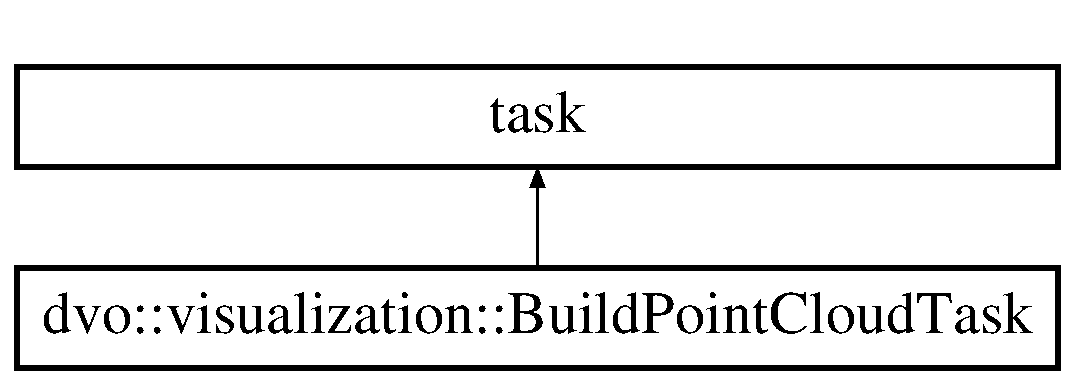
\includegraphics[height=2.000000cm]{classdvo_1_1visualization_1_1_build_point_cloud_task}
\end{center}
\end{figure}
\subsection*{Public Member Functions}
\begin{DoxyCompactItemize}
\item 
\mbox{\hyperlink{classdvo_1_1visualization_1_1_build_point_cloud_task_a86d5efbdab6f61d69949d86291a568ee}{Build\+Point\+Cloud\+Task}} (const dvo\+::core\+::\+Rgbd\+Image \&image, const dvo\+::core\+::\+Intrinsic\+Matrix \&intrinsics, const Eigen\+::\+Affine3d \&pose, Async\+Point\+Cloud\+Builder\+::\+Done\+Callback \&callback)
\item 
virtual \mbox{\hyperlink{classdvo_1_1visualization_1_1_build_point_cloud_task_a36ec8829378677b87aca9dd3ef9c5a68}{$\sim$\+Build\+Point\+Cloud\+Task}} ()
\item 
virtual tbb\+::task $\ast$ \mbox{\hyperlink{classdvo_1_1visualization_1_1_build_point_cloud_task_aa9ee4ddd7a6ed4fda80328ed542b7f03}{execute}} ()
\end{DoxyCompactItemize}


\subsection{Constructor \& Destructor Documentation}
\mbox{\Hypertarget{classdvo_1_1visualization_1_1_build_point_cloud_task_a86d5efbdab6f61d69949d86291a568ee}\label{classdvo_1_1visualization_1_1_build_point_cloud_task_a86d5efbdab6f61d69949d86291a568ee}} 
\index{dvo\+::visualization\+::\+Build\+Point\+Cloud\+Task@{dvo\+::visualization\+::\+Build\+Point\+Cloud\+Task}!Build\+Point\+Cloud\+Task@{Build\+Point\+Cloud\+Task}}
\index{Build\+Point\+Cloud\+Task@{Build\+Point\+Cloud\+Task}!dvo\+::visualization\+::\+Build\+Point\+Cloud\+Task@{dvo\+::visualization\+::\+Build\+Point\+Cloud\+Task}}
\subsubsection{\texorpdfstring{Build\+Point\+Cloud\+Task()}{BuildPointCloudTask()}}
{\footnotesize\ttfamily dvo\+::visualization\+::\+Build\+Point\+Cloud\+Task\+::\+Build\+Point\+Cloud\+Task (\begin{DoxyParamCaption}\item[{const dvo\+::core\+::\+Rgbd\+Image \&}]{image,  }\item[{const dvo\+::core\+::\+Intrinsic\+Matrix \&}]{intrinsics,  }\item[{const Eigen\+::\+Affine3d \&}]{pose,  }\item[{Async\+Point\+Cloud\+Builder\+::\+Done\+Callback \&}]{callback }\end{DoxyParamCaption})\hspace{0.3cm}{\ttfamily [inline]}}

\mbox{\Hypertarget{classdvo_1_1visualization_1_1_build_point_cloud_task_a36ec8829378677b87aca9dd3ef9c5a68}\label{classdvo_1_1visualization_1_1_build_point_cloud_task_a36ec8829378677b87aca9dd3ef9c5a68}} 
\index{dvo\+::visualization\+::\+Build\+Point\+Cloud\+Task@{dvo\+::visualization\+::\+Build\+Point\+Cloud\+Task}!````~Build\+Point\+Cloud\+Task@{$\sim$\+Build\+Point\+Cloud\+Task}}
\index{````~Build\+Point\+Cloud\+Task@{$\sim$\+Build\+Point\+Cloud\+Task}!dvo\+::visualization\+::\+Build\+Point\+Cloud\+Task@{dvo\+::visualization\+::\+Build\+Point\+Cloud\+Task}}
\subsubsection{\texorpdfstring{$\sim$\+Build\+Point\+Cloud\+Task()}{~BuildPointCloudTask()}}
{\footnotesize\ttfamily virtual dvo\+::visualization\+::\+Build\+Point\+Cloud\+Task\+::$\sim$\+Build\+Point\+Cloud\+Task (\begin{DoxyParamCaption}{ }\end{DoxyParamCaption})\hspace{0.3cm}{\ttfamily [inline]}, {\ttfamily [virtual]}}



\subsection{Member Function Documentation}
\mbox{\Hypertarget{classdvo_1_1visualization_1_1_build_point_cloud_task_aa9ee4ddd7a6ed4fda80328ed542b7f03}\label{classdvo_1_1visualization_1_1_build_point_cloud_task_aa9ee4ddd7a6ed4fda80328ed542b7f03}} 
\index{dvo\+::visualization\+::\+Build\+Point\+Cloud\+Task@{dvo\+::visualization\+::\+Build\+Point\+Cloud\+Task}!execute@{execute}}
\index{execute@{execute}!dvo\+::visualization\+::\+Build\+Point\+Cloud\+Task@{dvo\+::visualization\+::\+Build\+Point\+Cloud\+Task}}
\subsubsection{\texorpdfstring{execute()}{execute()}}
{\footnotesize\ttfamily virtual tbb\+::task$\ast$ dvo\+::visualization\+::\+Build\+Point\+Cloud\+Task\+::execute (\begin{DoxyParamCaption}{ }\end{DoxyParamCaption})\hspace{0.3cm}{\ttfamily [inline]}, {\ttfamily [virtual]}}



The documentation for this class was generated from the following file\+:\begin{DoxyCompactItemize}
\item 
visualization/\mbox{\hyperlink{async__point__cloud__builder_8cpp}{async\+\_\+point\+\_\+cloud\+\_\+builder.\+cpp}}\end{DoxyCompactItemize}

\hypertarget{structdvo_1_1visualization_1_1_visualizer_impl_1_1_create_histogram_func}{}\section{dvo\+:\+:visualization\+:\+:Visualizer\+Impl\+:\+:Create\+Histogram\+Func Struct Reference}
\label{structdvo_1_1visualization_1_1_visualizer_impl_1_1_create_histogram_func}\index{dvo\+::visualization\+::\+Visualizer\+Impl\+::\+Create\+Histogram\+Func@{dvo\+::visualization\+::\+Visualizer\+Impl\+::\+Create\+Histogram\+Func}}
\subsection*{Public Member Functions}
\begin{DoxyCompactItemize}
\item 
\mbox{\hyperlink{structdvo_1_1visualization_1_1_visualizer_impl_1_1_create_histogram_func_a46119b239b3abe5149e87476909c9261}{Create\+Histogram\+Func}} ()
\item 
\mbox{\hyperlink{structdvo_1_1visualization_1_1_visualizer_impl_1_1_create_histogram_func_a69be68ff5c6076f3476ded29bae27459}{Create\+Histogram\+Func}} (\mbox{\hyperlink{classdvo_1_1visualization_1_1_visualizer_impl}{Visualizer\+Impl}} $\ast$\mbox{\hyperlink{structdvo_1_1visualization_1_1_visualizer_impl_1_1_create_histogram_func_ae19bb1f928d400acb2e3fc28abfcbc1f}{impl}}, std\+::string \&\mbox{\hyperlink{structdvo_1_1visualization_1_1_visualizer_impl_1_1_create_histogram_func_a638ab4faaac71fc668bc6fb5e5c507b1}{name}}, const cv\+::\+Mat \&\mbox{\hyperlink{structdvo_1_1visualization_1_1_visualizer_impl_1_1_create_histogram_func_a7952450e28b9783d240be3c97e5fcbcf}{img}}, float \mbox{\hyperlink{structdvo_1_1visualization_1_1_visualizer_impl_1_1_create_histogram_func_a717312061e68d056ae466ff779fdbb4d}{binsize}}, float \mbox{\hyperlink{structdvo_1_1visualization_1_1_visualizer_impl_1_1_create_histogram_func_a8e2240d16aa20296dd4972aec744d3c4}{min}}, float \mbox{\hyperlink{structdvo_1_1visualization_1_1_visualizer_impl_1_1_create_histogram_func_a3065555b8878be3836e64f3b72bc2d01}{max}})
\item 
\mbox{\hyperlink{structdvo_1_1visualization_1_1_visualizer_impl_1_1_create_histogram_func_ad293baffb04f6bdd3708fa0e7f57488b}{Create\+Histogram\+Func}} (const \mbox{\hyperlink{structdvo_1_1visualization_1_1_visualizer_impl_1_1_create_histogram_func}{Create\+Histogram\+Func}} \&other)
\item 
\mbox{\hyperlink{structdvo_1_1visualization_1_1_visualizer_impl_1_1_create_histogram_func_a41c1677190f0ad86b52d904ec39c7f62}{$\sim$\+Create\+Histogram\+Func}} ()
\item 
void \mbox{\hyperlink{structdvo_1_1visualization_1_1_visualizer_impl_1_1_create_histogram_func_a51f624a7cfc68750daabaa7f72b37a58}{operator()}} ()
\item 
void \mbox{\hyperlink{structdvo_1_1visualization_1_1_visualizer_impl_1_1_create_histogram_func_a1cc5af2ecf024459deb1cd18dcd9cacc}{save}} (std\+::string filename)
\end{DoxyCompactItemize}
\subsection*{Public Attributes}
\begin{DoxyCompactItemize}
\item 
\mbox{\hyperlink{classdvo_1_1visualization_1_1_visualizer_impl}{Visualizer\+Impl}} $\ast$ \mbox{\hyperlink{structdvo_1_1visualization_1_1_visualizer_impl_1_1_create_histogram_func_ae19bb1f928d400acb2e3fc28abfcbc1f}{impl}}
\item 
std\+::string \mbox{\hyperlink{structdvo_1_1visualization_1_1_visualizer_impl_1_1_create_histogram_func_a638ab4faaac71fc668bc6fb5e5c507b1}{name}}
\item 
cv\+::\+Mat \mbox{\hyperlink{structdvo_1_1visualization_1_1_visualizer_impl_1_1_create_histogram_func_a7952450e28b9783d240be3c97e5fcbcf}{img}}
\item 
float \mbox{\hyperlink{structdvo_1_1visualization_1_1_visualizer_impl_1_1_create_histogram_func_a717312061e68d056ae466ff779fdbb4d}{binsize}}
\item 
float \mbox{\hyperlink{structdvo_1_1visualization_1_1_visualizer_impl_1_1_create_histogram_func_a8e2240d16aa20296dd4972aec744d3c4}{min}}
\item 
float \mbox{\hyperlink{structdvo_1_1visualization_1_1_visualizer_impl_1_1_create_histogram_func_a3065555b8878be3836e64f3b72bc2d01}{max}}
\end{DoxyCompactItemize}


\subsection{Constructor \& Destructor Documentation}
\mbox{\Hypertarget{structdvo_1_1visualization_1_1_visualizer_impl_1_1_create_histogram_func_a46119b239b3abe5149e87476909c9261}\label{structdvo_1_1visualization_1_1_visualizer_impl_1_1_create_histogram_func_a46119b239b3abe5149e87476909c9261}} 
\index{dvo\+::visualization\+::\+Visualizer\+Impl\+::\+Create\+Histogram\+Func@{dvo\+::visualization\+::\+Visualizer\+Impl\+::\+Create\+Histogram\+Func}!Create\+Histogram\+Func@{Create\+Histogram\+Func}}
\index{Create\+Histogram\+Func@{Create\+Histogram\+Func}!dvo\+::visualization\+::\+Visualizer\+Impl\+::\+Create\+Histogram\+Func@{dvo\+::visualization\+::\+Visualizer\+Impl\+::\+Create\+Histogram\+Func}}
\subsubsection{\texorpdfstring{Create\+Histogram\+Func()}{CreateHistogramFunc()}\hspace{0.1cm}{\footnotesize\ttfamily [1/3]}}
{\footnotesize\ttfamily dvo\+::visualization\+::\+Visualizer\+Impl\+::\+Create\+Histogram\+Func\+::\+Create\+Histogram\+Func (\begin{DoxyParamCaption}{ }\end{DoxyParamCaption})\hspace{0.3cm}{\ttfamily [inline]}}

\mbox{\Hypertarget{structdvo_1_1visualization_1_1_visualizer_impl_1_1_create_histogram_func_a69be68ff5c6076f3476ded29bae27459}\label{structdvo_1_1visualization_1_1_visualizer_impl_1_1_create_histogram_func_a69be68ff5c6076f3476ded29bae27459}} 
\index{dvo\+::visualization\+::\+Visualizer\+Impl\+::\+Create\+Histogram\+Func@{dvo\+::visualization\+::\+Visualizer\+Impl\+::\+Create\+Histogram\+Func}!Create\+Histogram\+Func@{Create\+Histogram\+Func}}
\index{Create\+Histogram\+Func@{Create\+Histogram\+Func}!dvo\+::visualization\+::\+Visualizer\+Impl\+::\+Create\+Histogram\+Func@{dvo\+::visualization\+::\+Visualizer\+Impl\+::\+Create\+Histogram\+Func}}
\subsubsection{\texorpdfstring{Create\+Histogram\+Func()}{CreateHistogramFunc()}\hspace{0.1cm}{\footnotesize\ttfamily [2/3]}}
{\footnotesize\ttfamily dvo\+::visualization\+::\+Visualizer\+Impl\+::\+Create\+Histogram\+Func\+::\+Create\+Histogram\+Func (\begin{DoxyParamCaption}\item[{\mbox{\hyperlink{classdvo_1_1visualization_1_1_visualizer_impl}{Visualizer\+Impl}} $\ast$}]{impl,  }\item[{std\+::string \&}]{name,  }\item[{const cv\+::\+Mat \&}]{img,  }\item[{float}]{binsize,  }\item[{float}]{min,  }\item[{float}]{max }\end{DoxyParamCaption})\hspace{0.3cm}{\ttfamily [inline]}}

\mbox{\Hypertarget{structdvo_1_1visualization_1_1_visualizer_impl_1_1_create_histogram_func_ad293baffb04f6bdd3708fa0e7f57488b}\label{structdvo_1_1visualization_1_1_visualizer_impl_1_1_create_histogram_func_ad293baffb04f6bdd3708fa0e7f57488b}} 
\index{dvo\+::visualization\+::\+Visualizer\+Impl\+::\+Create\+Histogram\+Func@{dvo\+::visualization\+::\+Visualizer\+Impl\+::\+Create\+Histogram\+Func}!Create\+Histogram\+Func@{Create\+Histogram\+Func}}
\index{Create\+Histogram\+Func@{Create\+Histogram\+Func}!dvo\+::visualization\+::\+Visualizer\+Impl\+::\+Create\+Histogram\+Func@{dvo\+::visualization\+::\+Visualizer\+Impl\+::\+Create\+Histogram\+Func}}
\subsubsection{\texorpdfstring{Create\+Histogram\+Func()}{CreateHistogramFunc()}\hspace{0.1cm}{\footnotesize\ttfamily [3/3]}}
{\footnotesize\ttfamily dvo\+::visualization\+::\+Visualizer\+Impl\+::\+Create\+Histogram\+Func\+::\+Create\+Histogram\+Func (\begin{DoxyParamCaption}\item[{const \mbox{\hyperlink{structdvo_1_1visualization_1_1_visualizer_impl_1_1_create_histogram_func}{Create\+Histogram\+Func}} \&}]{other }\end{DoxyParamCaption})\hspace{0.3cm}{\ttfamily [inline]}}

\mbox{\Hypertarget{structdvo_1_1visualization_1_1_visualizer_impl_1_1_create_histogram_func_a41c1677190f0ad86b52d904ec39c7f62}\label{structdvo_1_1visualization_1_1_visualizer_impl_1_1_create_histogram_func_a41c1677190f0ad86b52d904ec39c7f62}} 
\index{dvo\+::visualization\+::\+Visualizer\+Impl\+::\+Create\+Histogram\+Func@{dvo\+::visualization\+::\+Visualizer\+Impl\+::\+Create\+Histogram\+Func}!````~Create\+Histogram\+Func@{$\sim$\+Create\+Histogram\+Func}}
\index{````~Create\+Histogram\+Func@{$\sim$\+Create\+Histogram\+Func}!dvo\+::visualization\+::\+Visualizer\+Impl\+::\+Create\+Histogram\+Func@{dvo\+::visualization\+::\+Visualizer\+Impl\+::\+Create\+Histogram\+Func}}
\subsubsection{\texorpdfstring{$\sim$\+Create\+Histogram\+Func()}{~CreateHistogramFunc()}}
{\footnotesize\ttfamily dvo\+::visualization\+::\+Visualizer\+Impl\+::\+Create\+Histogram\+Func\+::$\sim$\+Create\+Histogram\+Func (\begin{DoxyParamCaption}{ }\end{DoxyParamCaption})\hspace{0.3cm}{\ttfamily [inline]}}



\subsection{Member Function Documentation}
\mbox{\Hypertarget{structdvo_1_1visualization_1_1_visualizer_impl_1_1_create_histogram_func_a51f624a7cfc68750daabaa7f72b37a58}\label{structdvo_1_1visualization_1_1_visualizer_impl_1_1_create_histogram_func_a51f624a7cfc68750daabaa7f72b37a58}} 
\index{dvo\+::visualization\+::\+Visualizer\+Impl\+::\+Create\+Histogram\+Func@{dvo\+::visualization\+::\+Visualizer\+Impl\+::\+Create\+Histogram\+Func}!operator()@{operator()}}
\index{operator()@{operator()}!dvo\+::visualization\+::\+Visualizer\+Impl\+::\+Create\+Histogram\+Func@{dvo\+::visualization\+::\+Visualizer\+Impl\+::\+Create\+Histogram\+Func}}
\subsubsection{\texorpdfstring{operator()()}{operator()()}}
{\footnotesize\ttfamily void dvo\+::visualization\+::\+Visualizer\+Impl\+::\+Create\+Histogram\+Func\+::operator() (\begin{DoxyParamCaption}{ }\end{DoxyParamCaption})\hspace{0.3cm}{\ttfamily [inline]}}

\mbox{\Hypertarget{structdvo_1_1visualization_1_1_visualizer_impl_1_1_create_histogram_func_a1cc5af2ecf024459deb1cd18dcd9cacc}\label{structdvo_1_1visualization_1_1_visualizer_impl_1_1_create_histogram_func_a1cc5af2ecf024459deb1cd18dcd9cacc}} 
\index{dvo\+::visualization\+::\+Visualizer\+Impl\+::\+Create\+Histogram\+Func@{dvo\+::visualization\+::\+Visualizer\+Impl\+::\+Create\+Histogram\+Func}!save@{save}}
\index{save@{save}!dvo\+::visualization\+::\+Visualizer\+Impl\+::\+Create\+Histogram\+Func@{dvo\+::visualization\+::\+Visualizer\+Impl\+::\+Create\+Histogram\+Func}}
\subsubsection{\texorpdfstring{save()}{save()}}
{\footnotesize\ttfamily void dvo\+::visualization\+::\+Visualizer\+Impl\+::\+Create\+Histogram\+Func\+::save (\begin{DoxyParamCaption}\item[{std\+::string}]{filename }\end{DoxyParamCaption})\hspace{0.3cm}{\ttfamily [inline]}}



\subsection{Member Data Documentation}
\mbox{\Hypertarget{structdvo_1_1visualization_1_1_visualizer_impl_1_1_create_histogram_func_a717312061e68d056ae466ff779fdbb4d}\label{structdvo_1_1visualization_1_1_visualizer_impl_1_1_create_histogram_func_a717312061e68d056ae466ff779fdbb4d}} 
\index{dvo\+::visualization\+::\+Visualizer\+Impl\+::\+Create\+Histogram\+Func@{dvo\+::visualization\+::\+Visualizer\+Impl\+::\+Create\+Histogram\+Func}!binsize@{binsize}}
\index{binsize@{binsize}!dvo\+::visualization\+::\+Visualizer\+Impl\+::\+Create\+Histogram\+Func@{dvo\+::visualization\+::\+Visualizer\+Impl\+::\+Create\+Histogram\+Func}}
\subsubsection{\texorpdfstring{binsize}{binsize}}
{\footnotesize\ttfamily float dvo\+::visualization\+::\+Visualizer\+Impl\+::\+Create\+Histogram\+Func\+::binsize}

\mbox{\Hypertarget{structdvo_1_1visualization_1_1_visualizer_impl_1_1_create_histogram_func_a7952450e28b9783d240be3c97e5fcbcf}\label{structdvo_1_1visualization_1_1_visualizer_impl_1_1_create_histogram_func_a7952450e28b9783d240be3c97e5fcbcf}} 
\index{dvo\+::visualization\+::\+Visualizer\+Impl\+::\+Create\+Histogram\+Func@{dvo\+::visualization\+::\+Visualizer\+Impl\+::\+Create\+Histogram\+Func}!img@{img}}
\index{img@{img}!dvo\+::visualization\+::\+Visualizer\+Impl\+::\+Create\+Histogram\+Func@{dvo\+::visualization\+::\+Visualizer\+Impl\+::\+Create\+Histogram\+Func}}
\subsubsection{\texorpdfstring{img}{img}}
{\footnotesize\ttfamily cv\+::\+Mat dvo\+::visualization\+::\+Visualizer\+Impl\+::\+Create\+Histogram\+Func\+::img}

\mbox{\Hypertarget{structdvo_1_1visualization_1_1_visualizer_impl_1_1_create_histogram_func_ae19bb1f928d400acb2e3fc28abfcbc1f}\label{structdvo_1_1visualization_1_1_visualizer_impl_1_1_create_histogram_func_ae19bb1f928d400acb2e3fc28abfcbc1f}} 
\index{dvo\+::visualization\+::\+Visualizer\+Impl\+::\+Create\+Histogram\+Func@{dvo\+::visualization\+::\+Visualizer\+Impl\+::\+Create\+Histogram\+Func}!impl@{impl}}
\index{impl@{impl}!dvo\+::visualization\+::\+Visualizer\+Impl\+::\+Create\+Histogram\+Func@{dvo\+::visualization\+::\+Visualizer\+Impl\+::\+Create\+Histogram\+Func}}
\subsubsection{\texorpdfstring{impl}{impl}}
{\footnotesize\ttfamily \mbox{\hyperlink{classdvo_1_1visualization_1_1_visualizer_impl}{Visualizer\+Impl}}$\ast$ dvo\+::visualization\+::\+Visualizer\+Impl\+::\+Create\+Histogram\+Func\+::impl}

\mbox{\Hypertarget{structdvo_1_1visualization_1_1_visualizer_impl_1_1_create_histogram_func_a3065555b8878be3836e64f3b72bc2d01}\label{structdvo_1_1visualization_1_1_visualizer_impl_1_1_create_histogram_func_a3065555b8878be3836e64f3b72bc2d01}} 
\index{dvo\+::visualization\+::\+Visualizer\+Impl\+::\+Create\+Histogram\+Func@{dvo\+::visualization\+::\+Visualizer\+Impl\+::\+Create\+Histogram\+Func}!max@{max}}
\index{max@{max}!dvo\+::visualization\+::\+Visualizer\+Impl\+::\+Create\+Histogram\+Func@{dvo\+::visualization\+::\+Visualizer\+Impl\+::\+Create\+Histogram\+Func}}
\subsubsection{\texorpdfstring{max}{max}}
{\footnotesize\ttfamily float dvo\+::visualization\+::\+Visualizer\+Impl\+::\+Create\+Histogram\+Func\+::max}

\mbox{\Hypertarget{structdvo_1_1visualization_1_1_visualizer_impl_1_1_create_histogram_func_a8e2240d16aa20296dd4972aec744d3c4}\label{structdvo_1_1visualization_1_1_visualizer_impl_1_1_create_histogram_func_a8e2240d16aa20296dd4972aec744d3c4}} 
\index{dvo\+::visualization\+::\+Visualizer\+Impl\+::\+Create\+Histogram\+Func@{dvo\+::visualization\+::\+Visualizer\+Impl\+::\+Create\+Histogram\+Func}!min@{min}}
\index{min@{min}!dvo\+::visualization\+::\+Visualizer\+Impl\+::\+Create\+Histogram\+Func@{dvo\+::visualization\+::\+Visualizer\+Impl\+::\+Create\+Histogram\+Func}}
\subsubsection{\texorpdfstring{min}{min}}
{\footnotesize\ttfamily float dvo\+::visualization\+::\+Visualizer\+Impl\+::\+Create\+Histogram\+Func\+::min}

\mbox{\Hypertarget{structdvo_1_1visualization_1_1_visualizer_impl_1_1_create_histogram_func_a638ab4faaac71fc668bc6fb5e5c507b1}\label{structdvo_1_1visualization_1_1_visualizer_impl_1_1_create_histogram_func_a638ab4faaac71fc668bc6fb5e5c507b1}} 
\index{dvo\+::visualization\+::\+Visualizer\+Impl\+::\+Create\+Histogram\+Func@{dvo\+::visualization\+::\+Visualizer\+Impl\+::\+Create\+Histogram\+Func}!name@{name}}
\index{name@{name}!dvo\+::visualization\+::\+Visualizer\+Impl\+::\+Create\+Histogram\+Func@{dvo\+::visualization\+::\+Visualizer\+Impl\+::\+Create\+Histogram\+Func}}
\subsubsection{\texorpdfstring{name}{name}}
{\footnotesize\ttfamily std\+::string dvo\+::visualization\+::\+Visualizer\+Impl\+::\+Create\+Histogram\+Func\+::name}



The documentation for this struct was generated from the following file\+:\begin{DoxyCompactItemize}
\item 
visualization/\mbox{\hyperlink{visualizer_8cpp}{visualizer.\+cpp}}\end{DoxyCompactItemize}

\hypertarget{structdvo_1_1_least_squares_equations_reduction}{}\section{dvo\+:\+:Least\+Squares\+Equations\+Reduction Struct Reference}
\label{structdvo_1_1_least_squares_equations_reduction}\index{dvo\+::\+Least\+Squares\+Equations\+Reduction@{dvo\+::\+Least\+Squares\+Equations\+Reduction}}
\subsection*{Public Member Functions}
\begin{DoxyCompactItemize}
\item 
\mbox{\hyperlink{structdvo_1_1_least_squares_equations_reduction_ae69114a4911fd35ce60a4696d15ce5a1}{Least\+Squares\+Equations\+Reduction}} (const cv\+::\+Mat \&\mbox{\hyperlink{structdvo_1_1_least_squares_equations_reduction_a6140e6f4c600016951877b7f79efeec1}{residuals}}, const dvo\+::core\+::\+Weight\+Calculation \&\mbox{\hyperlink{structdvo_1_1_least_squares_equations_reduction_a135763297b1e3bcee21189e0f5014fe4}{weights}}, const cv\+::\+Mat \&\mbox{\hyperlink{structdvo_1_1_least_squares_equations_reduction_a513436c876416261efe1d99188f8117a}{Jix}}, const cv\+::\+Mat \&\mbox{\hyperlink{structdvo_1_1_least_squares_equations_reduction_a7d8b6e08f0baf9580e0d5eb00776911f}{Jiy}}, const dvo\+::core\+::\+Rgbd\+Image\+::\+Point\+Cloud \&\mbox{\hyperlink{structdvo_1_1_least_squares_equations_reduction_a31ca8e056a271c3f3c99140e679a55c1}{points}})
\item 
\mbox{\hyperlink{structdvo_1_1_least_squares_equations_reduction_a0d615509ae3ef7176e8f9504065de1b0}{Least\+Squares\+Equations\+Reduction}} (\mbox{\hyperlink{structdvo_1_1_least_squares_equations_reduction}{Least\+Squares\+Equations\+Reduction}} \&other, tbb\+::split)
\item 
\mbox{\hyperlink{structdvo_1_1_least_squares_equations_reduction_aebf5509fd667020911a060bb93df51c2}{$\sim$\+Least\+Squares\+Equations\+Reduction}} ()
\item 
void \mbox{\hyperlink{structdvo_1_1_least_squares_equations_reduction_a4730c4255382ba919c088e70cbea9d44}{operator()}} (const tbb\+::blocked\+\_\+range$<$ size\+\_\+t $>$ \&r)
\item 
void \mbox{\hyperlink{structdvo_1_1_least_squares_equations_reduction_a35553c6631e0ff25089aea292619bf6b}{join}} (\mbox{\hyperlink{structdvo_1_1_least_squares_equations_reduction}{Least\+Squares\+Equations\+Reduction}} \&other)
\end{DoxyCompactItemize}
\subsection*{Public Attributes}
\begin{DoxyCompactItemize}
\item 
dvo\+::core\+::\+Normal\+Equations\+Least\+Squares $\ast$ \mbox{\hyperlink{structdvo_1_1_least_squares_equations_reduction_a3af436ffa51a579212c4e1e913a4350b}{ls}}
\item 
const cv\+::\+Mat \& \mbox{\hyperlink{structdvo_1_1_least_squares_equations_reduction_a6140e6f4c600016951877b7f79efeec1}{residuals}}
\item 
const cv\+::\+Mat \mbox{\hyperlink{structdvo_1_1_least_squares_equations_reduction_a513436c876416261efe1d99188f8117a}{Jix}}
\item 
const cv\+::\+Mat \mbox{\hyperlink{structdvo_1_1_least_squares_equations_reduction_a7d8b6e08f0baf9580e0d5eb00776911f}{Jiy}}
\item 
const dvo\+::core\+::\+Rgbd\+Image\+::\+Point\+Cloud \& \mbox{\hyperlink{structdvo_1_1_least_squares_equations_reduction_a31ca8e056a271c3f3c99140e679a55c1}{points}}
\item 
const dvo\+::core\+::\+Weight\+Calculation \& \mbox{\hyperlink{structdvo_1_1_least_squares_equations_reduction_a135763297b1e3bcee21189e0f5014fe4}{weights}}
\end{DoxyCompactItemize}


\subsection{Constructor \& Destructor Documentation}
\mbox{\Hypertarget{structdvo_1_1_least_squares_equations_reduction_ae69114a4911fd35ce60a4696d15ce5a1}\label{structdvo_1_1_least_squares_equations_reduction_ae69114a4911fd35ce60a4696d15ce5a1}} 
\index{dvo\+::\+Least\+Squares\+Equations\+Reduction@{dvo\+::\+Least\+Squares\+Equations\+Reduction}!Least\+Squares\+Equations\+Reduction@{Least\+Squares\+Equations\+Reduction}}
\index{Least\+Squares\+Equations\+Reduction@{Least\+Squares\+Equations\+Reduction}!dvo\+::\+Least\+Squares\+Equations\+Reduction@{dvo\+::\+Least\+Squares\+Equations\+Reduction}}
\subsubsection{\texorpdfstring{Least\+Squares\+Equations\+Reduction()}{LeastSquaresEquationsReduction()}\hspace{0.1cm}{\footnotesize\ttfamily [1/2]}}
{\footnotesize\ttfamily dvo\+::\+Least\+Squares\+Equations\+Reduction\+::\+Least\+Squares\+Equations\+Reduction (\begin{DoxyParamCaption}\item[{const cv\+::\+Mat \&}]{residuals,  }\item[{const dvo\+::core\+::\+Weight\+Calculation \&}]{weights,  }\item[{const cv\+::\+Mat \&}]{Jix,  }\item[{const cv\+::\+Mat \&}]{Jiy,  }\item[{const dvo\+::core\+::\+Rgbd\+Image\+::\+Point\+Cloud \&}]{points }\end{DoxyParamCaption})\hspace{0.3cm}{\ttfamily [inline]}}

\mbox{\Hypertarget{structdvo_1_1_least_squares_equations_reduction_a0d615509ae3ef7176e8f9504065de1b0}\label{structdvo_1_1_least_squares_equations_reduction_a0d615509ae3ef7176e8f9504065de1b0}} 
\index{dvo\+::\+Least\+Squares\+Equations\+Reduction@{dvo\+::\+Least\+Squares\+Equations\+Reduction}!Least\+Squares\+Equations\+Reduction@{Least\+Squares\+Equations\+Reduction}}
\index{Least\+Squares\+Equations\+Reduction@{Least\+Squares\+Equations\+Reduction}!dvo\+::\+Least\+Squares\+Equations\+Reduction@{dvo\+::\+Least\+Squares\+Equations\+Reduction}}
\subsubsection{\texorpdfstring{Least\+Squares\+Equations\+Reduction()}{LeastSquaresEquationsReduction()}\hspace{0.1cm}{\footnotesize\ttfamily [2/2]}}
{\footnotesize\ttfamily dvo\+::\+Least\+Squares\+Equations\+Reduction\+::\+Least\+Squares\+Equations\+Reduction (\begin{DoxyParamCaption}\item[{\mbox{\hyperlink{structdvo_1_1_least_squares_equations_reduction}{Least\+Squares\+Equations\+Reduction}} \&}]{other,  }\item[{tbb\+::split}]{ }\end{DoxyParamCaption})\hspace{0.3cm}{\ttfamily [inline]}}

\mbox{\Hypertarget{structdvo_1_1_least_squares_equations_reduction_aebf5509fd667020911a060bb93df51c2}\label{structdvo_1_1_least_squares_equations_reduction_aebf5509fd667020911a060bb93df51c2}} 
\index{dvo\+::\+Least\+Squares\+Equations\+Reduction@{dvo\+::\+Least\+Squares\+Equations\+Reduction}!````~Least\+Squares\+Equations\+Reduction@{$\sim$\+Least\+Squares\+Equations\+Reduction}}
\index{````~Least\+Squares\+Equations\+Reduction@{$\sim$\+Least\+Squares\+Equations\+Reduction}!dvo\+::\+Least\+Squares\+Equations\+Reduction@{dvo\+::\+Least\+Squares\+Equations\+Reduction}}
\subsubsection{\texorpdfstring{$\sim$\+Least\+Squares\+Equations\+Reduction()}{~LeastSquaresEquationsReduction()}}
{\footnotesize\ttfamily dvo\+::\+Least\+Squares\+Equations\+Reduction\+::$\sim$\+Least\+Squares\+Equations\+Reduction (\begin{DoxyParamCaption}{ }\end{DoxyParamCaption})\hspace{0.3cm}{\ttfamily [inline]}}



\subsection{Member Function Documentation}
\mbox{\Hypertarget{structdvo_1_1_least_squares_equations_reduction_a35553c6631e0ff25089aea292619bf6b}\label{structdvo_1_1_least_squares_equations_reduction_a35553c6631e0ff25089aea292619bf6b}} 
\index{dvo\+::\+Least\+Squares\+Equations\+Reduction@{dvo\+::\+Least\+Squares\+Equations\+Reduction}!join@{join}}
\index{join@{join}!dvo\+::\+Least\+Squares\+Equations\+Reduction@{dvo\+::\+Least\+Squares\+Equations\+Reduction}}
\subsubsection{\texorpdfstring{join()}{join()}}
{\footnotesize\ttfamily void dvo\+::\+Least\+Squares\+Equations\+Reduction\+::join (\begin{DoxyParamCaption}\item[{\mbox{\hyperlink{structdvo_1_1_least_squares_equations_reduction}{Least\+Squares\+Equations\+Reduction}} \&}]{other }\end{DoxyParamCaption})\hspace{0.3cm}{\ttfamily [inline]}}

\mbox{\Hypertarget{structdvo_1_1_least_squares_equations_reduction_a4730c4255382ba919c088e70cbea9d44}\label{structdvo_1_1_least_squares_equations_reduction_a4730c4255382ba919c088e70cbea9d44}} 
\index{dvo\+::\+Least\+Squares\+Equations\+Reduction@{dvo\+::\+Least\+Squares\+Equations\+Reduction}!operator()@{operator()}}
\index{operator()@{operator()}!dvo\+::\+Least\+Squares\+Equations\+Reduction@{dvo\+::\+Least\+Squares\+Equations\+Reduction}}
\subsubsection{\texorpdfstring{operator()()}{operator()()}}
{\footnotesize\ttfamily void dvo\+::\+Least\+Squares\+Equations\+Reduction\+::operator() (\begin{DoxyParamCaption}\item[{const tbb\+::blocked\+\_\+range$<$ size\+\_\+t $>$ \&}]{r }\end{DoxyParamCaption})\hspace{0.3cm}{\ttfamily [inline]}}



\subsection{Member Data Documentation}
\mbox{\Hypertarget{structdvo_1_1_least_squares_equations_reduction_a513436c876416261efe1d99188f8117a}\label{structdvo_1_1_least_squares_equations_reduction_a513436c876416261efe1d99188f8117a}} 
\index{dvo\+::\+Least\+Squares\+Equations\+Reduction@{dvo\+::\+Least\+Squares\+Equations\+Reduction}!Jix@{Jix}}
\index{Jix@{Jix}!dvo\+::\+Least\+Squares\+Equations\+Reduction@{dvo\+::\+Least\+Squares\+Equations\+Reduction}}
\subsubsection{\texorpdfstring{Jix}{Jix}}
{\footnotesize\ttfamily const cv\+::\+Mat dvo\+::\+Least\+Squares\+Equations\+Reduction\+::\+Jix}

\mbox{\Hypertarget{structdvo_1_1_least_squares_equations_reduction_a7d8b6e08f0baf9580e0d5eb00776911f}\label{structdvo_1_1_least_squares_equations_reduction_a7d8b6e08f0baf9580e0d5eb00776911f}} 
\index{dvo\+::\+Least\+Squares\+Equations\+Reduction@{dvo\+::\+Least\+Squares\+Equations\+Reduction}!Jiy@{Jiy}}
\index{Jiy@{Jiy}!dvo\+::\+Least\+Squares\+Equations\+Reduction@{dvo\+::\+Least\+Squares\+Equations\+Reduction}}
\subsubsection{\texorpdfstring{Jiy}{Jiy}}
{\footnotesize\ttfamily const cv\+::\+Mat dvo\+::\+Least\+Squares\+Equations\+Reduction\+::\+Jiy}

\mbox{\Hypertarget{structdvo_1_1_least_squares_equations_reduction_a3af436ffa51a579212c4e1e913a4350b}\label{structdvo_1_1_least_squares_equations_reduction_a3af436ffa51a579212c4e1e913a4350b}} 
\index{dvo\+::\+Least\+Squares\+Equations\+Reduction@{dvo\+::\+Least\+Squares\+Equations\+Reduction}!ls@{ls}}
\index{ls@{ls}!dvo\+::\+Least\+Squares\+Equations\+Reduction@{dvo\+::\+Least\+Squares\+Equations\+Reduction}}
\subsubsection{\texorpdfstring{ls}{ls}}
{\footnotesize\ttfamily dvo\+::core\+::\+Normal\+Equations\+Least\+Squares$\ast$ dvo\+::\+Least\+Squares\+Equations\+Reduction\+::ls}

\mbox{\Hypertarget{structdvo_1_1_least_squares_equations_reduction_a31ca8e056a271c3f3c99140e679a55c1}\label{structdvo_1_1_least_squares_equations_reduction_a31ca8e056a271c3f3c99140e679a55c1}} 
\index{dvo\+::\+Least\+Squares\+Equations\+Reduction@{dvo\+::\+Least\+Squares\+Equations\+Reduction}!points@{points}}
\index{points@{points}!dvo\+::\+Least\+Squares\+Equations\+Reduction@{dvo\+::\+Least\+Squares\+Equations\+Reduction}}
\subsubsection{\texorpdfstring{points}{points}}
{\footnotesize\ttfamily const dvo\+::core\+::\+Rgbd\+Image\+::\+Point\+Cloud\& dvo\+::\+Least\+Squares\+Equations\+Reduction\+::points}

\mbox{\Hypertarget{structdvo_1_1_least_squares_equations_reduction_a6140e6f4c600016951877b7f79efeec1}\label{structdvo_1_1_least_squares_equations_reduction_a6140e6f4c600016951877b7f79efeec1}} 
\index{dvo\+::\+Least\+Squares\+Equations\+Reduction@{dvo\+::\+Least\+Squares\+Equations\+Reduction}!residuals@{residuals}}
\index{residuals@{residuals}!dvo\+::\+Least\+Squares\+Equations\+Reduction@{dvo\+::\+Least\+Squares\+Equations\+Reduction}}
\subsubsection{\texorpdfstring{residuals}{residuals}}
{\footnotesize\ttfamily const cv\+::\+Mat\& dvo\+::\+Least\+Squares\+Equations\+Reduction\+::residuals}

\mbox{\Hypertarget{structdvo_1_1_least_squares_equations_reduction_a135763297b1e3bcee21189e0f5014fe4}\label{structdvo_1_1_least_squares_equations_reduction_a135763297b1e3bcee21189e0f5014fe4}} 
\index{dvo\+::\+Least\+Squares\+Equations\+Reduction@{dvo\+::\+Least\+Squares\+Equations\+Reduction}!weights@{weights}}
\index{weights@{weights}!dvo\+::\+Least\+Squares\+Equations\+Reduction@{dvo\+::\+Least\+Squares\+Equations\+Reduction}}
\subsubsection{\texorpdfstring{weights}{weights}}
{\footnotesize\ttfamily const dvo\+::core\+::\+Weight\+Calculation\& dvo\+::\+Least\+Squares\+Equations\+Reduction\+::weights}



The documentation for this struct was generated from the following file\+:\begin{DoxyCompactItemize}
\item 
\mbox{\hyperlink{dense__tracking_8cpp}{dense\+\_\+tracking.\+cpp}}\end{DoxyCompactItemize}

\hypertarget{structdvo_1_1visualization_1_1_visualizer_impl_1_1_named_image}{}\section{dvo\+:\+:visualization\+:\+:Visualizer\+Impl\+:\+:Named\+Image Struct Reference}
\label{structdvo_1_1visualization_1_1_visualizer_impl_1_1_named_image}\index{dvo\+::visualization\+::\+Visualizer\+Impl\+::\+Named\+Image@{dvo\+::visualization\+::\+Visualizer\+Impl\+::\+Named\+Image}}
\subsection*{Public Member Functions}
\begin{DoxyCompactItemize}
\item 
\mbox{\hyperlink{structdvo_1_1visualization_1_1_visualizer_impl_1_1_named_image_ad8d49d26aa2b0fd5166857b2ee913489}{Named\+Image}} ()
\item 
\mbox{\hyperlink{structdvo_1_1visualization_1_1_visualizer_impl_1_1_named_image_a85ef82568b83987428230f90bc4c00a2}{Named\+Image}} (std\+::string \&\mbox{\hyperlink{structdvo_1_1visualization_1_1_visualizer_impl_1_1_named_image_aa46e7e1b17cd744452ba8ef3dffddfe7}{name}}, const cv\+::\+Mat\+Expr \&\mbox{\hyperlink{structdvo_1_1visualization_1_1_visualizer_impl_1_1_named_image_a7ff904dac2fc68f459ee05a32abf3cea}{img}}, Visualizer\+::\+Image\+Modifier \&\mbox{\hyperlink{structdvo_1_1visualization_1_1_visualizer_impl_1_1_named_image_a831a0937bdfc9427f20669770f37f1d0}{modifier}})
\end{DoxyCompactItemize}
\subsection*{Public Attributes}
\begin{DoxyCompactItemize}
\item 
std\+::string \mbox{\hyperlink{structdvo_1_1visualization_1_1_visualizer_impl_1_1_named_image_aa46e7e1b17cd744452ba8ef3dffddfe7}{name}}
\item 
cv\+::\+Mat\+Expr \mbox{\hyperlink{structdvo_1_1visualization_1_1_visualizer_impl_1_1_named_image_a7ff904dac2fc68f459ee05a32abf3cea}{img}}
\item 
Visualizer\+::\+Image\+Modifier \mbox{\hyperlink{structdvo_1_1visualization_1_1_visualizer_impl_1_1_named_image_a831a0937bdfc9427f20669770f37f1d0}{modifier}}
\end{DoxyCompactItemize}


\subsection{Constructor \& Destructor Documentation}
\mbox{\Hypertarget{structdvo_1_1visualization_1_1_visualizer_impl_1_1_named_image_ad8d49d26aa2b0fd5166857b2ee913489}\label{structdvo_1_1visualization_1_1_visualizer_impl_1_1_named_image_ad8d49d26aa2b0fd5166857b2ee913489}} 
\index{dvo\+::visualization\+::\+Visualizer\+Impl\+::\+Named\+Image@{dvo\+::visualization\+::\+Visualizer\+Impl\+::\+Named\+Image}!Named\+Image@{Named\+Image}}
\index{Named\+Image@{Named\+Image}!dvo\+::visualization\+::\+Visualizer\+Impl\+::\+Named\+Image@{dvo\+::visualization\+::\+Visualizer\+Impl\+::\+Named\+Image}}
\subsubsection{\texorpdfstring{Named\+Image()}{NamedImage()}\hspace{0.1cm}{\footnotesize\ttfamily [1/2]}}
{\footnotesize\ttfamily dvo\+::visualization\+::\+Visualizer\+Impl\+::\+Named\+Image\+::\+Named\+Image (\begin{DoxyParamCaption}{ }\end{DoxyParamCaption})\hspace{0.3cm}{\ttfamily [inline]}}

\mbox{\Hypertarget{structdvo_1_1visualization_1_1_visualizer_impl_1_1_named_image_a85ef82568b83987428230f90bc4c00a2}\label{structdvo_1_1visualization_1_1_visualizer_impl_1_1_named_image_a85ef82568b83987428230f90bc4c00a2}} 
\index{dvo\+::visualization\+::\+Visualizer\+Impl\+::\+Named\+Image@{dvo\+::visualization\+::\+Visualizer\+Impl\+::\+Named\+Image}!Named\+Image@{Named\+Image}}
\index{Named\+Image@{Named\+Image}!dvo\+::visualization\+::\+Visualizer\+Impl\+::\+Named\+Image@{dvo\+::visualization\+::\+Visualizer\+Impl\+::\+Named\+Image}}
\subsubsection{\texorpdfstring{Named\+Image()}{NamedImage()}\hspace{0.1cm}{\footnotesize\ttfamily [2/2]}}
{\footnotesize\ttfamily dvo\+::visualization\+::\+Visualizer\+Impl\+::\+Named\+Image\+::\+Named\+Image (\begin{DoxyParamCaption}\item[{std\+::string \&}]{name,  }\item[{const cv\+::\+Mat\+Expr \&}]{img,  }\item[{Visualizer\+::\+Image\+Modifier \&}]{modifier }\end{DoxyParamCaption})\hspace{0.3cm}{\ttfamily [inline]}}



\subsection{Member Data Documentation}
\mbox{\Hypertarget{structdvo_1_1visualization_1_1_visualizer_impl_1_1_named_image_a7ff904dac2fc68f459ee05a32abf3cea}\label{structdvo_1_1visualization_1_1_visualizer_impl_1_1_named_image_a7ff904dac2fc68f459ee05a32abf3cea}} 
\index{dvo\+::visualization\+::\+Visualizer\+Impl\+::\+Named\+Image@{dvo\+::visualization\+::\+Visualizer\+Impl\+::\+Named\+Image}!img@{img}}
\index{img@{img}!dvo\+::visualization\+::\+Visualizer\+Impl\+::\+Named\+Image@{dvo\+::visualization\+::\+Visualizer\+Impl\+::\+Named\+Image}}
\subsubsection{\texorpdfstring{img}{img}}
{\footnotesize\ttfamily cv\+::\+Mat\+Expr dvo\+::visualization\+::\+Visualizer\+Impl\+::\+Named\+Image\+::img}

\mbox{\Hypertarget{structdvo_1_1visualization_1_1_visualizer_impl_1_1_named_image_a831a0937bdfc9427f20669770f37f1d0}\label{structdvo_1_1visualization_1_1_visualizer_impl_1_1_named_image_a831a0937bdfc9427f20669770f37f1d0}} 
\index{dvo\+::visualization\+::\+Visualizer\+Impl\+::\+Named\+Image@{dvo\+::visualization\+::\+Visualizer\+Impl\+::\+Named\+Image}!modifier@{modifier}}
\index{modifier@{modifier}!dvo\+::visualization\+::\+Visualizer\+Impl\+::\+Named\+Image@{dvo\+::visualization\+::\+Visualizer\+Impl\+::\+Named\+Image}}
\subsubsection{\texorpdfstring{modifier}{modifier}}
{\footnotesize\ttfamily Visualizer\+::\+Image\+Modifier dvo\+::visualization\+::\+Visualizer\+Impl\+::\+Named\+Image\+::modifier}

\mbox{\Hypertarget{structdvo_1_1visualization_1_1_visualizer_impl_1_1_named_image_aa46e7e1b17cd744452ba8ef3dffddfe7}\label{structdvo_1_1visualization_1_1_visualizer_impl_1_1_named_image_aa46e7e1b17cd744452ba8ef3dffddfe7}} 
\index{dvo\+::visualization\+::\+Visualizer\+Impl\+::\+Named\+Image@{dvo\+::visualization\+::\+Visualizer\+Impl\+::\+Named\+Image}!name@{name}}
\index{name@{name}!dvo\+::visualization\+::\+Visualizer\+Impl\+::\+Named\+Image@{dvo\+::visualization\+::\+Visualizer\+Impl\+::\+Named\+Image}}
\subsubsection{\texorpdfstring{name}{name}}
{\footnotesize\ttfamily std\+::string dvo\+::visualization\+::\+Visualizer\+Impl\+::\+Named\+Image\+::name}



The documentation for this struct was generated from the following file\+:\begin{DoxyCompactItemize}
\item 
visualization/\mbox{\hyperlink{visualizer_8cpp}{visualizer.\+cpp}}\end{DoxyCompactItemize}

\hypertarget{classdvo_1_1visualization_1_1_noop_camera_visualizer}{}\section{dvo\+:\+:visualization\+:\+:Noop\+Camera\+Visualizer Class Reference}
\label{classdvo_1_1visualization_1_1_noop_camera_visualizer}\index{dvo\+::visualization\+::\+Noop\+Camera\+Visualizer@{dvo\+::visualization\+::\+Noop\+Camera\+Visualizer}}
Inheritance diagram for dvo\+:\+:visualization\+:\+:Noop\+Camera\+Visualizer\+:\begin{figure}[H]
\begin{center}
\leavevmode
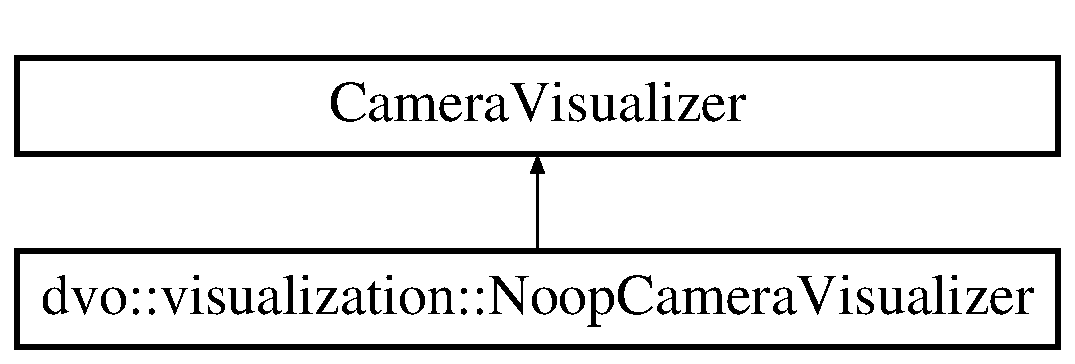
\includegraphics[height=2.000000cm]{classdvo_1_1visualization_1_1_noop_camera_visualizer}
\end{center}
\end{figure}
\subsection*{Public Member Functions}
\begin{DoxyCompactItemize}
\item 
\mbox{\hyperlink{classdvo_1_1visualization_1_1_noop_camera_visualizer_ade3cb140e752ade11e25f0ad049958af}{Noop\+Camera\+Visualizer}} ()
\item 
virtual \mbox{\hyperlink{classdvo_1_1visualization_1_1_noop_camera_visualizer_ae29e589ff8c183b11c1d2ac8e6072447}{$\sim$\+Noop\+Camera\+Visualizer}} ()
\item 
virtual void \mbox{\hyperlink{classdvo_1_1visualization_1_1_noop_camera_visualizer_acfb97efacfcb9e3dd30444e34c7bfd9c}{show}} (Option option=Show\+Camera\+And\+Cloud)
\item 
virtual void \mbox{\hyperlink{classdvo_1_1visualization_1_1_noop_camera_visualizer_a875ff591e3db513ddbec48478989639e}{hide}} ()
\item 
virtual Camera\+Visualizer \& \mbox{\hyperlink{classdvo_1_1visualization_1_1_noop_camera_visualizer_a7983d8de9de45c5617c3e877d36d6ff3}{update}} (const dvo\+::core\+::\+Rgbd\+Image \&img, const dvo\+::core\+::\+Intrinsic\+Matrix \&intrinsics, const Eigen\+::\+Affine3d \&pose)
\end{DoxyCompactItemize}


\subsection{Constructor \& Destructor Documentation}
\mbox{\Hypertarget{classdvo_1_1visualization_1_1_noop_camera_visualizer_ade3cb140e752ade11e25f0ad049958af}\label{classdvo_1_1visualization_1_1_noop_camera_visualizer_ade3cb140e752ade11e25f0ad049958af}} 
\index{dvo\+::visualization\+::\+Noop\+Camera\+Visualizer@{dvo\+::visualization\+::\+Noop\+Camera\+Visualizer}!Noop\+Camera\+Visualizer@{Noop\+Camera\+Visualizer}}
\index{Noop\+Camera\+Visualizer@{Noop\+Camera\+Visualizer}!dvo\+::visualization\+::\+Noop\+Camera\+Visualizer@{dvo\+::visualization\+::\+Noop\+Camera\+Visualizer}}
\subsubsection{\texorpdfstring{Noop\+Camera\+Visualizer()}{NoopCameraVisualizer()}}
{\footnotesize\ttfamily dvo\+::visualization\+::\+Noop\+Camera\+Visualizer\+::\+Noop\+Camera\+Visualizer (\begin{DoxyParamCaption}{ }\end{DoxyParamCaption})\hspace{0.3cm}{\ttfamily [inline]}}

\mbox{\Hypertarget{classdvo_1_1visualization_1_1_noop_camera_visualizer_ae29e589ff8c183b11c1d2ac8e6072447}\label{classdvo_1_1visualization_1_1_noop_camera_visualizer_ae29e589ff8c183b11c1d2ac8e6072447}} 
\index{dvo\+::visualization\+::\+Noop\+Camera\+Visualizer@{dvo\+::visualization\+::\+Noop\+Camera\+Visualizer}!````~Noop\+Camera\+Visualizer@{$\sim$\+Noop\+Camera\+Visualizer}}
\index{````~Noop\+Camera\+Visualizer@{$\sim$\+Noop\+Camera\+Visualizer}!dvo\+::visualization\+::\+Noop\+Camera\+Visualizer@{dvo\+::visualization\+::\+Noop\+Camera\+Visualizer}}
\subsubsection{\texorpdfstring{$\sim$\+Noop\+Camera\+Visualizer()}{~NoopCameraVisualizer()}}
{\footnotesize\ttfamily virtual dvo\+::visualization\+::\+Noop\+Camera\+Visualizer\+::$\sim$\+Noop\+Camera\+Visualizer (\begin{DoxyParamCaption}{ }\end{DoxyParamCaption})\hspace{0.3cm}{\ttfamily [inline]}, {\ttfamily [virtual]}}



\subsection{Member Function Documentation}
\mbox{\Hypertarget{classdvo_1_1visualization_1_1_noop_camera_visualizer_a875ff591e3db513ddbec48478989639e}\label{classdvo_1_1visualization_1_1_noop_camera_visualizer_a875ff591e3db513ddbec48478989639e}} 
\index{dvo\+::visualization\+::\+Noop\+Camera\+Visualizer@{dvo\+::visualization\+::\+Noop\+Camera\+Visualizer}!hide@{hide}}
\index{hide@{hide}!dvo\+::visualization\+::\+Noop\+Camera\+Visualizer@{dvo\+::visualization\+::\+Noop\+Camera\+Visualizer}}
\subsubsection{\texorpdfstring{hide()}{hide()}}
{\footnotesize\ttfamily virtual void dvo\+::visualization\+::\+Noop\+Camera\+Visualizer\+::hide (\begin{DoxyParamCaption}{ }\end{DoxyParamCaption})\hspace{0.3cm}{\ttfamily [inline]}, {\ttfamily [virtual]}}

\mbox{\Hypertarget{classdvo_1_1visualization_1_1_noop_camera_visualizer_acfb97efacfcb9e3dd30444e34c7bfd9c}\label{classdvo_1_1visualization_1_1_noop_camera_visualizer_acfb97efacfcb9e3dd30444e34c7bfd9c}} 
\index{dvo\+::visualization\+::\+Noop\+Camera\+Visualizer@{dvo\+::visualization\+::\+Noop\+Camera\+Visualizer}!show@{show}}
\index{show@{show}!dvo\+::visualization\+::\+Noop\+Camera\+Visualizer@{dvo\+::visualization\+::\+Noop\+Camera\+Visualizer}}
\subsubsection{\texorpdfstring{show()}{show()}}
{\footnotesize\ttfamily virtual void dvo\+::visualization\+::\+Noop\+Camera\+Visualizer\+::show (\begin{DoxyParamCaption}\item[{Option}]{option = {\ttfamily ShowCameraAndCloud} }\end{DoxyParamCaption})\hspace{0.3cm}{\ttfamily [inline]}, {\ttfamily [virtual]}}

\mbox{\Hypertarget{classdvo_1_1visualization_1_1_noop_camera_visualizer_a7983d8de9de45c5617c3e877d36d6ff3}\label{classdvo_1_1visualization_1_1_noop_camera_visualizer_a7983d8de9de45c5617c3e877d36d6ff3}} 
\index{dvo\+::visualization\+::\+Noop\+Camera\+Visualizer@{dvo\+::visualization\+::\+Noop\+Camera\+Visualizer}!update@{update}}
\index{update@{update}!dvo\+::visualization\+::\+Noop\+Camera\+Visualizer@{dvo\+::visualization\+::\+Noop\+Camera\+Visualizer}}
\subsubsection{\texorpdfstring{update()}{update()}}
{\footnotesize\ttfamily virtual Camera\+Visualizer\& dvo\+::visualization\+::\+Noop\+Camera\+Visualizer\+::update (\begin{DoxyParamCaption}\item[{const dvo\+::core\+::\+Rgbd\+Image \&}]{img,  }\item[{const dvo\+::core\+::\+Intrinsic\+Matrix \&}]{intrinsics,  }\item[{const Eigen\+::\+Affine3d \&}]{pose }\end{DoxyParamCaption})\hspace{0.3cm}{\ttfamily [inline]}, {\ttfamily [virtual]}}



The documentation for this class was generated from the following file\+:\begin{DoxyCompactItemize}
\item 
visualization/\mbox{\hyperlink{camera__trajectory__visualizer_8cpp}{camera\+\_\+trajectory\+\_\+visualizer.\+cpp}}\end{DoxyCompactItemize}

\hypertarget{classdvo_1_1visualization_1_1_noop_trajectory_visualizer}{}\section{dvo\+:\+:visualization\+:\+:Noop\+Trajectory\+Visualizer Class Reference}
\label{classdvo_1_1visualization_1_1_noop_trajectory_visualizer}\index{dvo\+::visualization\+::\+Noop\+Trajectory\+Visualizer@{dvo\+::visualization\+::\+Noop\+Trajectory\+Visualizer}}
Inheritance diagram for dvo\+:\+:visualization\+:\+:Noop\+Trajectory\+Visualizer\+:\begin{figure}[H]
\begin{center}
\leavevmode
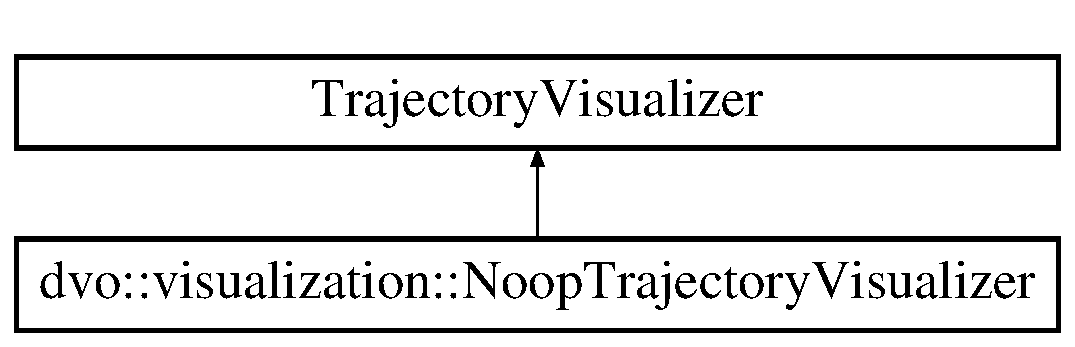
\includegraphics[height=2.000000cm]{classdvo_1_1visualization_1_1_noop_trajectory_visualizer}
\end{center}
\end{figure}
\subsection*{Public Member Functions}
\begin{DoxyCompactItemize}
\item 
\mbox{\hyperlink{classdvo_1_1visualization_1_1_noop_trajectory_visualizer_a215b180a6d70948c2448ed7d0edc0852}{Noop\+Trajectory\+Visualizer}} ()
\item 
virtual \mbox{\hyperlink{classdvo_1_1visualization_1_1_noop_trajectory_visualizer_a2f3efe6c4bb5b294c72c594ef13060ca}{$\sim$\+Noop\+Trajectory\+Visualizer}} ()
\item 
virtual Trajectory\+Visualizer \& \mbox{\hyperlink{classdvo_1_1visualization_1_1_noop_trajectory_visualizer_a40e9cfd01744c3efa85afb93237e2030}{add}} (const Eigen\+::\+Affine3d \&pose)
\end{DoxyCompactItemize}


\subsection{Constructor \& Destructor Documentation}
\mbox{\Hypertarget{classdvo_1_1visualization_1_1_noop_trajectory_visualizer_a215b180a6d70948c2448ed7d0edc0852}\label{classdvo_1_1visualization_1_1_noop_trajectory_visualizer_a215b180a6d70948c2448ed7d0edc0852}} 
\index{dvo\+::visualization\+::\+Noop\+Trajectory\+Visualizer@{dvo\+::visualization\+::\+Noop\+Trajectory\+Visualizer}!Noop\+Trajectory\+Visualizer@{Noop\+Trajectory\+Visualizer}}
\index{Noop\+Trajectory\+Visualizer@{Noop\+Trajectory\+Visualizer}!dvo\+::visualization\+::\+Noop\+Trajectory\+Visualizer@{dvo\+::visualization\+::\+Noop\+Trajectory\+Visualizer}}
\subsubsection{\texorpdfstring{Noop\+Trajectory\+Visualizer()}{NoopTrajectoryVisualizer()}}
{\footnotesize\ttfamily dvo\+::visualization\+::\+Noop\+Trajectory\+Visualizer\+::\+Noop\+Trajectory\+Visualizer (\begin{DoxyParamCaption}{ }\end{DoxyParamCaption})\hspace{0.3cm}{\ttfamily [inline]}}

\mbox{\Hypertarget{classdvo_1_1visualization_1_1_noop_trajectory_visualizer_a2f3efe6c4bb5b294c72c594ef13060ca}\label{classdvo_1_1visualization_1_1_noop_trajectory_visualizer_a2f3efe6c4bb5b294c72c594ef13060ca}} 
\index{dvo\+::visualization\+::\+Noop\+Trajectory\+Visualizer@{dvo\+::visualization\+::\+Noop\+Trajectory\+Visualizer}!````~Noop\+Trajectory\+Visualizer@{$\sim$\+Noop\+Trajectory\+Visualizer}}
\index{````~Noop\+Trajectory\+Visualizer@{$\sim$\+Noop\+Trajectory\+Visualizer}!dvo\+::visualization\+::\+Noop\+Trajectory\+Visualizer@{dvo\+::visualization\+::\+Noop\+Trajectory\+Visualizer}}
\subsubsection{\texorpdfstring{$\sim$\+Noop\+Trajectory\+Visualizer()}{~NoopTrajectoryVisualizer()}}
{\footnotesize\ttfamily virtual dvo\+::visualization\+::\+Noop\+Trajectory\+Visualizer\+::$\sim$\+Noop\+Trajectory\+Visualizer (\begin{DoxyParamCaption}{ }\end{DoxyParamCaption})\hspace{0.3cm}{\ttfamily [inline]}, {\ttfamily [virtual]}}



\subsection{Member Function Documentation}
\mbox{\Hypertarget{classdvo_1_1visualization_1_1_noop_trajectory_visualizer_a40e9cfd01744c3efa85afb93237e2030}\label{classdvo_1_1visualization_1_1_noop_trajectory_visualizer_a40e9cfd01744c3efa85afb93237e2030}} 
\index{dvo\+::visualization\+::\+Noop\+Trajectory\+Visualizer@{dvo\+::visualization\+::\+Noop\+Trajectory\+Visualizer}!add@{add}}
\index{add@{add}!dvo\+::visualization\+::\+Noop\+Trajectory\+Visualizer@{dvo\+::visualization\+::\+Noop\+Trajectory\+Visualizer}}
\subsubsection{\texorpdfstring{add()}{add()}}
{\footnotesize\ttfamily virtual Trajectory\+Visualizer\& dvo\+::visualization\+::\+Noop\+Trajectory\+Visualizer\+::add (\begin{DoxyParamCaption}\item[{const Eigen\+::\+Affine3d \&}]{pose }\end{DoxyParamCaption})\hspace{0.3cm}{\ttfamily [inline]}, {\ttfamily [virtual]}}



The documentation for this class was generated from the following file\+:\begin{DoxyCompactItemize}
\item 
visualization/\mbox{\hyperlink{camera__trajectory__visualizer_8cpp}{camera\+\_\+trajectory\+\_\+visualizer.\+cpp}}\end{DoxyCompactItemize}

\hypertarget{structdvo_1_1visualization_1_1internal_1_1_pcl_camera_trajectory_visualizer_impl}{}\section{dvo\+:\+:visualization\+:\+:internal\+:\+:Pcl\+Camera\+Trajectory\+Visualizer\+Impl Struct Reference}
\label{structdvo_1_1visualization_1_1internal_1_1_pcl_camera_trajectory_visualizer_impl}\index{dvo\+::visualization\+::internal\+::\+Pcl\+Camera\+Trajectory\+Visualizer\+Impl@{dvo\+::visualization\+::internal\+::\+Pcl\+Camera\+Trajectory\+Visualizer\+Impl}}
\subsection*{Public Types}
\begin{DoxyCompactItemize}
\item 
typedef boost\+::shared\+\_\+ptr$<$ \mbox{\hyperlink{classdvo_1_1visualization_1_1internal_1_1_pcl_camera_visualizer}{Pcl\+Camera\+Visualizer}} $>$ \mbox{\hyperlink{structdvo_1_1visualization_1_1internal_1_1_pcl_camera_trajectory_visualizer_impl_ae1f73988c3445cb504978879b5abd6b2}{Pcl\+Camera\+Visualizer\+Ptr}}
\item 
typedef boost\+::shared\+\_\+ptr$<$ \mbox{\hyperlink{classdvo_1_1visualization_1_1internal_1_1_pcl_trajectory_visualizer}{Pcl\+Trajectory\+Visualizer}} $>$ \mbox{\hyperlink{structdvo_1_1visualization_1_1internal_1_1_pcl_camera_trajectory_visualizer_impl_abefe7d40c9c28acf23b80fd55dc4a8bb}{Pcl\+Trajectory\+Visualizer\+Ptr}}
\item 
typedef std\+::map$<$ std\+::string, \mbox{\hyperlink{structdvo_1_1visualization_1_1internal_1_1_pcl_camera_trajectory_visualizer_impl_ae1f73988c3445cb504978879b5abd6b2}{Pcl\+Camera\+Visualizer\+Ptr}} $>$ \mbox{\hyperlink{structdvo_1_1visualization_1_1internal_1_1_pcl_camera_trajectory_visualizer_impl_a7d244b61749bfd33a2170d2fc8bfa8b3}{Camera\+Visualizer\+Map}}
\item 
typedef std\+::map$<$ std\+::string, \mbox{\hyperlink{structdvo_1_1visualization_1_1internal_1_1_pcl_camera_trajectory_visualizer_impl_abefe7d40c9c28acf23b80fd55dc4a8bb}{Pcl\+Trajectory\+Visualizer\+Ptr}} $>$ \mbox{\hyperlink{structdvo_1_1visualization_1_1internal_1_1_pcl_camera_trajectory_visualizer_impl_a97e643f8b8f24ab7e9b79b0961fd2af7}{Trajectory\+Visualizer\+Map}}
\end{DoxyCompactItemize}
\subsection*{Public Member Functions}
\begin{DoxyCompactItemize}
\item 
\mbox{\hyperlink{structdvo_1_1visualization_1_1internal_1_1_pcl_camera_trajectory_visualizer_impl_ac27a7fde4cc28672ebb5e65f80eb8865}{Pcl\+Camera\+Trajectory\+Visualizer\+Impl}} (bool render\+\_\+thread=true)
\item 
\mbox{\hyperlink{structdvo_1_1visualization_1_1internal_1_1_pcl_camera_trajectory_visualizer_impl_a3a8627e770ee2c18d07e79f921e60d16}{$\sim$\+Pcl\+Camera\+Trajectory\+Visualizer\+Impl}} ()
\item 
void \mbox{\hyperlink{structdvo_1_1visualization_1_1internal_1_1_pcl_camera_trajectory_visualizer_impl_a21c3f13d2d5ccb2f2913a08a421cd7fd}{bind\+Switch\+To\+Key}} (\mbox{\hyperlink{structdvo_1_1visualization_1_1_switch}{Switch}} \&s, std\+::string \&key)
\item 
pcl\+::visualization\+::\+P\+C\+L\+Visualizer \& \mbox{\hyperlink{structdvo_1_1visualization_1_1internal_1_1_pcl_camera_trajectory_visualizer_impl_a28159937aa1551faf546b827eddb3f44}{visualizer}} ()
\item 
\mbox{\hyperlink{classdvo_1_1visualization_1_1_camera_visualizer_a473ebecc62e1d4edba21027d858789a2}{Camera\+Visualizer\+::\+Ptr}} \mbox{\hyperlink{structdvo_1_1visualization_1_1internal_1_1_pcl_camera_trajectory_visualizer_impl_a1834a57c67d10cbeac37362c546d3575}{camera}} (std\+::string name)
\item 
\mbox{\hyperlink{classdvo_1_1visualization_1_1_trajectory_visualizer_aac33ef5979fe64ee33409f1afa977fd3}{Trajectory\+Visualizer\+::\+Ptr}} \mbox{\hyperlink{structdvo_1_1visualization_1_1internal_1_1_pcl_camera_trajectory_visualizer_impl_a603eeb0964ce83fff1e736003177661c}{trajectory}} (std\+::string name)
\item 
void \mbox{\hyperlink{structdvo_1_1visualization_1_1internal_1_1_pcl_camera_trajectory_visualizer_impl_a3b1dc7581be3c4e278d0a60678be494e}{reset}} ()
\item 
void \mbox{\hyperlink{structdvo_1_1visualization_1_1internal_1_1_pcl_camera_trajectory_visualizer_impl_a79a0458c9c30be3b18f9cbc3a0d4002f}{init\+Visualizer}} ()
\item 
void \mbox{\hyperlink{structdvo_1_1visualization_1_1internal_1_1_pcl_camera_trajectory_visualizer_impl_ae2b0083367d0b2955cf2f7adb18a1acb}{render}} (int milliseconds)
\end{DoxyCompactItemize}
\subsection*{Public Attributes}
\begin{DoxyCompactItemize}
\item 
boost\+::mutex \mbox{\hyperlink{structdvo_1_1visualization_1_1internal_1_1_pcl_camera_trajectory_visualizer_impl_add80c1ad58f55ec00c2ad0d08c0aaaac}{sync\+\_\+}}
\end{DoxyCompactItemize}


\subsection{Member Typedef Documentation}
\mbox{\Hypertarget{structdvo_1_1visualization_1_1internal_1_1_pcl_camera_trajectory_visualizer_impl_a7d244b61749bfd33a2170d2fc8bfa8b3}\label{structdvo_1_1visualization_1_1internal_1_1_pcl_camera_trajectory_visualizer_impl_a7d244b61749bfd33a2170d2fc8bfa8b3}} 
\index{dvo\+::visualization\+::internal\+::\+Pcl\+Camera\+Trajectory\+Visualizer\+Impl@{dvo\+::visualization\+::internal\+::\+Pcl\+Camera\+Trajectory\+Visualizer\+Impl}!Camera\+Visualizer\+Map@{Camera\+Visualizer\+Map}}
\index{Camera\+Visualizer\+Map@{Camera\+Visualizer\+Map}!dvo\+::visualization\+::internal\+::\+Pcl\+Camera\+Trajectory\+Visualizer\+Impl@{dvo\+::visualization\+::internal\+::\+Pcl\+Camera\+Trajectory\+Visualizer\+Impl}}
\subsubsection{\texorpdfstring{Camera\+Visualizer\+Map}{CameraVisualizerMap}}
{\footnotesize\ttfamily typedef std\+::map$<$std\+::string, \mbox{\hyperlink{structdvo_1_1visualization_1_1internal_1_1_pcl_camera_trajectory_visualizer_impl_ae1f73988c3445cb504978879b5abd6b2}{Pcl\+Camera\+Visualizer\+Ptr}}$>$ \mbox{\hyperlink{structdvo_1_1visualization_1_1internal_1_1_pcl_camera_trajectory_visualizer_impl_a7d244b61749bfd33a2170d2fc8bfa8b3}{dvo\+::visualization\+::internal\+::\+Pcl\+Camera\+Trajectory\+Visualizer\+Impl\+::\+Camera\+Visualizer\+Map}}}

\mbox{\Hypertarget{structdvo_1_1visualization_1_1internal_1_1_pcl_camera_trajectory_visualizer_impl_ae1f73988c3445cb504978879b5abd6b2}\label{structdvo_1_1visualization_1_1internal_1_1_pcl_camera_trajectory_visualizer_impl_ae1f73988c3445cb504978879b5abd6b2}} 
\index{dvo\+::visualization\+::internal\+::\+Pcl\+Camera\+Trajectory\+Visualizer\+Impl@{dvo\+::visualization\+::internal\+::\+Pcl\+Camera\+Trajectory\+Visualizer\+Impl}!Pcl\+Camera\+Visualizer\+Ptr@{Pcl\+Camera\+Visualizer\+Ptr}}
\index{Pcl\+Camera\+Visualizer\+Ptr@{Pcl\+Camera\+Visualizer\+Ptr}!dvo\+::visualization\+::internal\+::\+Pcl\+Camera\+Trajectory\+Visualizer\+Impl@{dvo\+::visualization\+::internal\+::\+Pcl\+Camera\+Trajectory\+Visualizer\+Impl}}
\subsubsection{\texorpdfstring{Pcl\+Camera\+Visualizer\+Ptr}{PclCameraVisualizerPtr}}
{\footnotesize\ttfamily typedef boost\+::shared\+\_\+ptr$<$\mbox{\hyperlink{classdvo_1_1visualization_1_1internal_1_1_pcl_camera_visualizer}{Pcl\+Camera\+Visualizer}}$>$ \mbox{\hyperlink{structdvo_1_1visualization_1_1internal_1_1_pcl_camera_trajectory_visualizer_impl_ae1f73988c3445cb504978879b5abd6b2}{dvo\+::visualization\+::internal\+::\+Pcl\+Camera\+Trajectory\+Visualizer\+Impl\+::\+Pcl\+Camera\+Visualizer\+Ptr}}}

\mbox{\Hypertarget{structdvo_1_1visualization_1_1internal_1_1_pcl_camera_trajectory_visualizer_impl_abefe7d40c9c28acf23b80fd55dc4a8bb}\label{structdvo_1_1visualization_1_1internal_1_1_pcl_camera_trajectory_visualizer_impl_abefe7d40c9c28acf23b80fd55dc4a8bb}} 
\index{dvo\+::visualization\+::internal\+::\+Pcl\+Camera\+Trajectory\+Visualizer\+Impl@{dvo\+::visualization\+::internal\+::\+Pcl\+Camera\+Trajectory\+Visualizer\+Impl}!Pcl\+Trajectory\+Visualizer\+Ptr@{Pcl\+Trajectory\+Visualizer\+Ptr}}
\index{Pcl\+Trajectory\+Visualizer\+Ptr@{Pcl\+Trajectory\+Visualizer\+Ptr}!dvo\+::visualization\+::internal\+::\+Pcl\+Camera\+Trajectory\+Visualizer\+Impl@{dvo\+::visualization\+::internal\+::\+Pcl\+Camera\+Trajectory\+Visualizer\+Impl}}
\subsubsection{\texorpdfstring{Pcl\+Trajectory\+Visualizer\+Ptr}{PclTrajectoryVisualizerPtr}}
{\footnotesize\ttfamily typedef boost\+::shared\+\_\+ptr$<$\mbox{\hyperlink{classdvo_1_1visualization_1_1internal_1_1_pcl_trajectory_visualizer}{Pcl\+Trajectory\+Visualizer}}$>$ \mbox{\hyperlink{structdvo_1_1visualization_1_1internal_1_1_pcl_camera_trajectory_visualizer_impl_abefe7d40c9c28acf23b80fd55dc4a8bb}{dvo\+::visualization\+::internal\+::\+Pcl\+Camera\+Trajectory\+Visualizer\+Impl\+::\+Pcl\+Trajectory\+Visualizer\+Ptr}}}

\mbox{\Hypertarget{structdvo_1_1visualization_1_1internal_1_1_pcl_camera_trajectory_visualizer_impl_a97e643f8b8f24ab7e9b79b0961fd2af7}\label{structdvo_1_1visualization_1_1internal_1_1_pcl_camera_trajectory_visualizer_impl_a97e643f8b8f24ab7e9b79b0961fd2af7}} 
\index{dvo\+::visualization\+::internal\+::\+Pcl\+Camera\+Trajectory\+Visualizer\+Impl@{dvo\+::visualization\+::internal\+::\+Pcl\+Camera\+Trajectory\+Visualizer\+Impl}!Trajectory\+Visualizer\+Map@{Trajectory\+Visualizer\+Map}}
\index{Trajectory\+Visualizer\+Map@{Trajectory\+Visualizer\+Map}!dvo\+::visualization\+::internal\+::\+Pcl\+Camera\+Trajectory\+Visualizer\+Impl@{dvo\+::visualization\+::internal\+::\+Pcl\+Camera\+Trajectory\+Visualizer\+Impl}}
\subsubsection{\texorpdfstring{Trajectory\+Visualizer\+Map}{TrajectoryVisualizerMap}}
{\footnotesize\ttfamily typedef std\+::map$<$std\+::string, \mbox{\hyperlink{structdvo_1_1visualization_1_1internal_1_1_pcl_camera_trajectory_visualizer_impl_abefe7d40c9c28acf23b80fd55dc4a8bb}{Pcl\+Trajectory\+Visualizer\+Ptr}}$>$ \mbox{\hyperlink{structdvo_1_1visualization_1_1internal_1_1_pcl_camera_trajectory_visualizer_impl_a97e643f8b8f24ab7e9b79b0961fd2af7}{dvo\+::visualization\+::internal\+::\+Pcl\+Camera\+Trajectory\+Visualizer\+Impl\+::\+Trajectory\+Visualizer\+Map}}}



\subsection{Constructor \& Destructor Documentation}
\mbox{\Hypertarget{structdvo_1_1visualization_1_1internal_1_1_pcl_camera_trajectory_visualizer_impl_ac27a7fde4cc28672ebb5e65f80eb8865}\label{structdvo_1_1visualization_1_1internal_1_1_pcl_camera_trajectory_visualizer_impl_ac27a7fde4cc28672ebb5e65f80eb8865}} 
\index{dvo\+::visualization\+::internal\+::\+Pcl\+Camera\+Trajectory\+Visualizer\+Impl@{dvo\+::visualization\+::internal\+::\+Pcl\+Camera\+Trajectory\+Visualizer\+Impl}!Pcl\+Camera\+Trajectory\+Visualizer\+Impl@{Pcl\+Camera\+Trajectory\+Visualizer\+Impl}}
\index{Pcl\+Camera\+Trajectory\+Visualizer\+Impl@{Pcl\+Camera\+Trajectory\+Visualizer\+Impl}!dvo\+::visualization\+::internal\+::\+Pcl\+Camera\+Trajectory\+Visualizer\+Impl@{dvo\+::visualization\+::internal\+::\+Pcl\+Camera\+Trajectory\+Visualizer\+Impl}}
\subsubsection{\texorpdfstring{Pcl\+Camera\+Trajectory\+Visualizer\+Impl()}{PclCameraTrajectoryVisualizerImpl()}}
{\footnotesize\ttfamily dvo\+::visualization\+::internal\+::\+Pcl\+Camera\+Trajectory\+Visualizer\+Impl\+::\+Pcl\+Camera\+Trajectory\+Visualizer\+Impl (\begin{DoxyParamCaption}\item[{bool}]{render\+\_\+thread = {\ttfamily true} }\end{DoxyParamCaption})\hspace{0.3cm}{\ttfamily [inline]}}

\mbox{\Hypertarget{structdvo_1_1visualization_1_1internal_1_1_pcl_camera_trajectory_visualizer_impl_a3a8627e770ee2c18d07e79f921e60d16}\label{structdvo_1_1visualization_1_1internal_1_1_pcl_camera_trajectory_visualizer_impl_a3a8627e770ee2c18d07e79f921e60d16}} 
\index{dvo\+::visualization\+::internal\+::\+Pcl\+Camera\+Trajectory\+Visualizer\+Impl@{dvo\+::visualization\+::internal\+::\+Pcl\+Camera\+Trajectory\+Visualizer\+Impl}!````~Pcl\+Camera\+Trajectory\+Visualizer\+Impl@{$\sim$\+Pcl\+Camera\+Trajectory\+Visualizer\+Impl}}
\index{````~Pcl\+Camera\+Trajectory\+Visualizer\+Impl@{$\sim$\+Pcl\+Camera\+Trajectory\+Visualizer\+Impl}!dvo\+::visualization\+::internal\+::\+Pcl\+Camera\+Trajectory\+Visualizer\+Impl@{dvo\+::visualization\+::internal\+::\+Pcl\+Camera\+Trajectory\+Visualizer\+Impl}}
\subsubsection{\texorpdfstring{$\sim$\+Pcl\+Camera\+Trajectory\+Visualizer\+Impl()}{~PclCameraTrajectoryVisualizerImpl()}}
{\footnotesize\ttfamily dvo\+::visualization\+::internal\+::\+Pcl\+Camera\+Trajectory\+Visualizer\+Impl\+::$\sim$\+Pcl\+Camera\+Trajectory\+Visualizer\+Impl (\begin{DoxyParamCaption}{ }\end{DoxyParamCaption})\hspace{0.3cm}{\ttfamily [inline]}}



\subsection{Member Function Documentation}
\mbox{\Hypertarget{structdvo_1_1visualization_1_1internal_1_1_pcl_camera_trajectory_visualizer_impl_a21c3f13d2d5ccb2f2913a08a421cd7fd}\label{structdvo_1_1visualization_1_1internal_1_1_pcl_camera_trajectory_visualizer_impl_a21c3f13d2d5ccb2f2913a08a421cd7fd}} 
\index{dvo\+::visualization\+::internal\+::\+Pcl\+Camera\+Trajectory\+Visualizer\+Impl@{dvo\+::visualization\+::internal\+::\+Pcl\+Camera\+Trajectory\+Visualizer\+Impl}!bind\+Switch\+To\+Key@{bind\+Switch\+To\+Key}}
\index{bind\+Switch\+To\+Key@{bind\+Switch\+To\+Key}!dvo\+::visualization\+::internal\+::\+Pcl\+Camera\+Trajectory\+Visualizer\+Impl@{dvo\+::visualization\+::internal\+::\+Pcl\+Camera\+Trajectory\+Visualizer\+Impl}}
\subsubsection{\texorpdfstring{bind\+Switch\+To\+Key()}{bindSwitchToKey()}}
{\footnotesize\ttfamily void dvo\+::visualization\+::internal\+::\+Pcl\+Camera\+Trajectory\+Visualizer\+Impl\+::bind\+Switch\+To\+Key (\begin{DoxyParamCaption}\item[{\mbox{\hyperlink{structdvo_1_1visualization_1_1_switch}{Switch}} \&}]{s,  }\item[{std\+::string \&}]{key }\end{DoxyParamCaption})\hspace{0.3cm}{\ttfamily [inline]}}

\mbox{\Hypertarget{structdvo_1_1visualization_1_1internal_1_1_pcl_camera_trajectory_visualizer_impl_a1834a57c67d10cbeac37362c546d3575}\label{structdvo_1_1visualization_1_1internal_1_1_pcl_camera_trajectory_visualizer_impl_a1834a57c67d10cbeac37362c546d3575}} 
\index{dvo\+::visualization\+::internal\+::\+Pcl\+Camera\+Trajectory\+Visualizer\+Impl@{dvo\+::visualization\+::internal\+::\+Pcl\+Camera\+Trajectory\+Visualizer\+Impl}!camera@{camera}}
\index{camera@{camera}!dvo\+::visualization\+::internal\+::\+Pcl\+Camera\+Trajectory\+Visualizer\+Impl@{dvo\+::visualization\+::internal\+::\+Pcl\+Camera\+Trajectory\+Visualizer\+Impl}}
\subsubsection{\texorpdfstring{camera()}{camera()}}
{\footnotesize\ttfamily \mbox{\hyperlink{classdvo_1_1visualization_1_1_camera_visualizer_a473ebecc62e1d4edba21027d858789a2}{Camera\+Visualizer\+::\+Ptr}} dvo\+::visualization\+::internal\+::\+Pcl\+Camera\+Trajectory\+Visualizer\+Impl\+::camera (\begin{DoxyParamCaption}\item[{std\+::string}]{name }\end{DoxyParamCaption})\hspace{0.3cm}{\ttfamily [inline]}}

\mbox{\Hypertarget{structdvo_1_1visualization_1_1internal_1_1_pcl_camera_trajectory_visualizer_impl_a79a0458c9c30be3b18f9cbc3a0d4002f}\label{structdvo_1_1visualization_1_1internal_1_1_pcl_camera_trajectory_visualizer_impl_a79a0458c9c30be3b18f9cbc3a0d4002f}} 
\index{dvo\+::visualization\+::internal\+::\+Pcl\+Camera\+Trajectory\+Visualizer\+Impl@{dvo\+::visualization\+::internal\+::\+Pcl\+Camera\+Trajectory\+Visualizer\+Impl}!init\+Visualizer@{init\+Visualizer}}
\index{init\+Visualizer@{init\+Visualizer}!dvo\+::visualization\+::internal\+::\+Pcl\+Camera\+Trajectory\+Visualizer\+Impl@{dvo\+::visualization\+::internal\+::\+Pcl\+Camera\+Trajectory\+Visualizer\+Impl}}
\subsubsection{\texorpdfstring{init\+Visualizer()}{initVisualizer()}}
{\footnotesize\ttfamily void dvo\+::visualization\+::internal\+::\+Pcl\+Camera\+Trajectory\+Visualizer\+Impl\+::init\+Visualizer (\begin{DoxyParamCaption}{ }\end{DoxyParamCaption})\hspace{0.3cm}{\ttfamily [inline]}}

\mbox{\Hypertarget{structdvo_1_1visualization_1_1internal_1_1_pcl_camera_trajectory_visualizer_impl_ae2b0083367d0b2955cf2f7adb18a1acb}\label{structdvo_1_1visualization_1_1internal_1_1_pcl_camera_trajectory_visualizer_impl_ae2b0083367d0b2955cf2f7adb18a1acb}} 
\index{dvo\+::visualization\+::internal\+::\+Pcl\+Camera\+Trajectory\+Visualizer\+Impl@{dvo\+::visualization\+::internal\+::\+Pcl\+Camera\+Trajectory\+Visualizer\+Impl}!render@{render}}
\index{render@{render}!dvo\+::visualization\+::internal\+::\+Pcl\+Camera\+Trajectory\+Visualizer\+Impl@{dvo\+::visualization\+::internal\+::\+Pcl\+Camera\+Trajectory\+Visualizer\+Impl}}
\subsubsection{\texorpdfstring{render()}{render()}}
{\footnotesize\ttfamily void dvo\+::visualization\+::internal\+::\+Pcl\+Camera\+Trajectory\+Visualizer\+Impl\+::render (\begin{DoxyParamCaption}\item[{int}]{milliseconds }\end{DoxyParamCaption})\hspace{0.3cm}{\ttfamily [inline]}}

\mbox{\Hypertarget{structdvo_1_1visualization_1_1internal_1_1_pcl_camera_trajectory_visualizer_impl_a3b1dc7581be3c4e278d0a60678be494e}\label{structdvo_1_1visualization_1_1internal_1_1_pcl_camera_trajectory_visualizer_impl_a3b1dc7581be3c4e278d0a60678be494e}} 
\index{dvo\+::visualization\+::internal\+::\+Pcl\+Camera\+Trajectory\+Visualizer\+Impl@{dvo\+::visualization\+::internal\+::\+Pcl\+Camera\+Trajectory\+Visualizer\+Impl}!reset@{reset}}
\index{reset@{reset}!dvo\+::visualization\+::internal\+::\+Pcl\+Camera\+Trajectory\+Visualizer\+Impl@{dvo\+::visualization\+::internal\+::\+Pcl\+Camera\+Trajectory\+Visualizer\+Impl}}
\subsubsection{\texorpdfstring{reset()}{reset()}}
{\footnotesize\ttfamily void dvo\+::visualization\+::internal\+::\+Pcl\+Camera\+Trajectory\+Visualizer\+Impl\+::reset (\begin{DoxyParamCaption}{ }\end{DoxyParamCaption})\hspace{0.3cm}{\ttfamily [inline]}}

\mbox{\Hypertarget{structdvo_1_1visualization_1_1internal_1_1_pcl_camera_trajectory_visualizer_impl_a603eeb0964ce83fff1e736003177661c}\label{structdvo_1_1visualization_1_1internal_1_1_pcl_camera_trajectory_visualizer_impl_a603eeb0964ce83fff1e736003177661c}} 
\index{dvo\+::visualization\+::internal\+::\+Pcl\+Camera\+Trajectory\+Visualizer\+Impl@{dvo\+::visualization\+::internal\+::\+Pcl\+Camera\+Trajectory\+Visualizer\+Impl}!trajectory@{trajectory}}
\index{trajectory@{trajectory}!dvo\+::visualization\+::internal\+::\+Pcl\+Camera\+Trajectory\+Visualizer\+Impl@{dvo\+::visualization\+::internal\+::\+Pcl\+Camera\+Trajectory\+Visualizer\+Impl}}
\subsubsection{\texorpdfstring{trajectory()}{trajectory()}}
{\footnotesize\ttfamily \mbox{\hyperlink{classdvo_1_1visualization_1_1_trajectory_visualizer_aac33ef5979fe64ee33409f1afa977fd3}{Trajectory\+Visualizer\+::\+Ptr}} dvo\+::visualization\+::internal\+::\+Pcl\+Camera\+Trajectory\+Visualizer\+Impl\+::trajectory (\begin{DoxyParamCaption}\item[{std\+::string}]{name }\end{DoxyParamCaption})\hspace{0.3cm}{\ttfamily [inline]}}

\mbox{\Hypertarget{structdvo_1_1visualization_1_1internal_1_1_pcl_camera_trajectory_visualizer_impl_a28159937aa1551faf546b827eddb3f44}\label{structdvo_1_1visualization_1_1internal_1_1_pcl_camera_trajectory_visualizer_impl_a28159937aa1551faf546b827eddb3f44}} 
\index{dvo\+::visualization\+::internal\+::\+Pcl\+Camera\+Trajectory\+Visualizer\+Impl@{dvo\+::visualization\+::internal\+::\+Pcl\+Camera\+Trajectory\+Visualizer\+Impl}!visualizer@{visualizer}}
\index{visualizer@{visualizer}!dvo\+::visualization\+::internal\+::\+Pcl\+Camera\+Trajectory\+Visualizer\+Impl@{dvo\+::visualization\+::internal\+::\+Pcl\+Camera\+Trajectory\+Visualizer\+Impl}}
\subsubsection{\texorpdfstring{visualizer()}{visualizer()}}
{\footnotesize\ttfamily pcl\+::visualization\+::\+P\+C\+L\+Visualizer\& dvo\+::visualization\+::internal\+::\+Pcl\+Camera\+Trajectory\+Visualizer\+Impl\+::visualizer (\begin{DoxyParamCaption}{ }\end{DoxyParamCaption})\hspace{0.3cm}{\ttfamily [inline]}}



\subsection{Member Data Documentation}
\mbox{\Hypertarget{structdvo_1_1visualization_1_1internal_1_1_pcl_camera_trajectory_visualizer_impl_add80c1ad58f55ec00c2ad0d08c0aaaac}\label{structdvo_1_1visualization_1_1internal_1_1_pcl_camera_trajectory_visualizer_impl_add80c1ad58f55ec00c2ad0d08c0aaaac}} 
\index{dvo\+::visualization\+::internal\+::\+Pcl\+Camera\+Trajectory\+Visualizer\+Impl@{dvo\+::visualization\+::internal\+::\+Pcl\+Camera\+Trajectory\+Visualizer\+Impl}!sync\+\_\+@{sync\+\_\+}}
\index{sync\+\_\+@{sync\+\_\+}!dvo\+::visualization\+::internal\+::\+Pcl\+Camera\+Trajectory\+Visualizer\+Impl@{dvo\+::visualization\+::internal\+::\+Pcl\+Camera\+Trajectory\+Visualizer\+Impl}}
\subsubsection{\texorpdfstring{sync\+\_\+}{sync\_}}
{\footnotesize\ttfamily boost\+::mutex dvo\+::visualization\+::internal\+::\+Pcl\+Camera\+Trajectory\+Visualizer\+Impl\+::sync\+\_\+}



The documentation for this struct was generated from the following file\+:\begin{DoxyCompactItemize}
\item 
dvo\+\_\+core/src/visualization/\mbox{\hyperlink{pcl__camera__trajetory__visualizer_8cpp}{pcl\+\_\+camera\+\_\+trajetory\+\_\+visualizer.\+cpp}}\end{DoxyCompactItemize}

\hypertarget{classdvo_1_1visualization_1_1internal_1_1_pcl_camera_visualizer}{}\section{dvo\+:\+:visualization\+:\+:internal\+:\+:Pcl\+Camera\+Visualizer Class Reference}
\label{classdvo_1_1visualization_1_1internal_1_1_pcl_camera_visualizer}\index{dvo\+::visualization\+::internal\+::\+Pcl\+Camera\+Visualizer@{dvo\+::visualization\+::internal\+::\+Pcl\+Camera\+Visualizer}}
Inheritance diagram for dvo\+:\+:visualization\+:\+:internal\+:\+:Pcl\+Camera\+Visualizer\+:\begin{figure}[H]
\begin{center}
\leavevmode
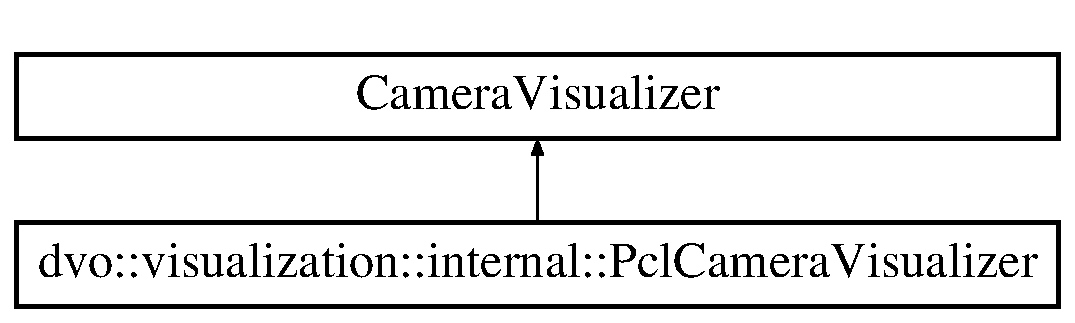
\includegraphics[height=2.000000cm]{classdvo_1_1visualization_1_1internal_1_1_pcl_camera_visualizer}
\end{center}
\end{figure}
\subsection*{Public Member Functions}
\begin{DoxyCompactItemize}
\item 
\mbox{\hyperlink{classdvo_1_1visualization_1_1internal_1_1_pcl_camera_visualizer_a4990540496b6a8104b6f3d794ed2bb17}{Pcl\+Camera\+Visualizer}} (std\+::string \&name)
\item 
virtual \mbox{\hyperlink{classdvo_1_1visualization_1_1internal_1_1_pcl_camera_visualizer_a594001de77ac60de8cd05a03d1314b8e}{$\sim$\+Pcl\+Camera\+Visualizer}} ()
\item 
virtual void \mbox{\hyperlink{classdvo_1_1visualization_1_1internal_1_1_pcl_camera_visualizer_a09b5d8117f8ca15489ac42f6b6019030}{show}} (Option option=Show\+Camera\+And\+Cloud)
\item 
virtual void \mbox{\hyperlink{classdvo_1_1visualization_1_1internal_1_1_pcl_camera_visualizer_ad261307239a87bc10ba4d0662960cc72}{hide}} ()
\item 
virtual Camera\+Visualizer \& \mbox{\hyperlink{classdvo_1_1visualization_1_1internal_1_1_pcl_camera_visualizer_adfe2b8752f78ee0fa6ee193be70941eb}{update}} (const dvo\+::core\+::\+Rgbd\+Image \&img, const dvo\+::core\+::\+Intrinsic\+Matrix \&intrinsics, const Eigen\+::\+Affine3d \&pose)
\item 
void \mbox{\hyperlink{classdvo_1_1visualization_1_1internal_1_1_pcl_camera_visualizer_adbc6ea5a07dace4e06773d568986424b}{update\+Visualizer}} (pcl\+::visualization\+::\+P\+C\+L\+Visualizer \&visualizer, Point\+Cloud\+Aggregator \&aggregator)
\end{DoxyCompactItemize}


\subsection{Constructor \& Destructor Documentation}
\mbox{\Hypertarget{classdvo_1_1visualization_1_1internal_1_1_pcl_camera_visualizer_a4990540496b6a8104b6f3d794ed2bb17}\label{classdvo_1_1visualization_1_1internal_1_1_pcl_camera_visualizer_a4990540496b6a8104b6f3d794ed2bb17}} 
\index{dvo\+::visualization\+::internal\+::\+Pcl\+Camera\+Visualizer@{dvo\+::visualization\+::internal\+::\+Pcl\+Camera\+Visualizer}!Pcl\+Camera\+Visualizer@{Pcl\+Camera\+Visualizer}}
\index{Pcl\+Camera\+Visualizer@{Pcl\+Camera\+Visualizer}!dvo\+::visualization\+::internal\+::\+Pcl\+Camera\+Visualizer@{dvo\+::visualization\+::internal\+::\+Pcl\+Camera\+Visualizer}}
\subsubsection{\texorpdfstring{Pcl\+Camera\+Visualizer()}{PclCameraVisualizer()}}
{\footnotesize\ttfamily dvo\+::visualization\+::internal\+::\+Pcl\+Camera\+Visualizer\+::\+Pcl\+Camera\+Visualizer (\begin{DoxyParamCaption}\item[{std\+::string \&}]{name }\end{DoxyParamCaption})\hspace{0.3cm}{\ttfamily [inline]}}

\mbox{\Hypertarget{classdvo_1_1visualization_1_1internal_1_1_pcl_camera_visualizer_a594001de77ac60de8cd05a03d1314b8e}\label{classdvo_1_1visualization_1_1internal_1_1_pcl_camera_visualizer_a594001de77ac60de8cd05a03d1314b8e}} 
\index{dvo\+::visualization\+::internal\+::\+Pcl\+Camera\+Visualizer@{dvo\+::visualization\+::internal\+::\+Pcl\+Camera\+Visualizer}!````~Pcl\+Camera\+Visualizer@{$\sim$\+Pcl\+Camera\+Visualizer}}
\index{````~Pcl\+Camera\+Visualizer@{$\sim$\+Pcl\+Camera\+Visualizer}!dvo\+::visualization\+::internal\+::\+Pcl\+Camera\+Visualizer@{dvo\+::visualization\+::internal\+::\+Pcl\+Camera\+Visualizer}}
\subsubsection{\texorpdfstring{$\sim$\+Pcl\+Camera\+Visualizer()}{~PclCameraVisualizer()}}
{\footnotesize\ttfamily virtual dvo\+::visualization\+::internal\+::\+Pcl\+Camera\+Visualizer\+::$\sim$\+Pcl\+Camera\+Visualizer (\begin{DoxyParamCaption}{ }\end{DoxyParamCaption})\hspace{0.3cm}{\ttfamily [inline]}, {\ttfamily [virtual]}}



\subsection{Member Function Documentation}
\mbox{\Hypertarget{classdvo_1_1visualization_1_1internal_1_1_pcl_camera_visualizer_ad261307239a87bc10ba4d0662960cc72}\label{classdvo_1_1visualization_1_1internal_1_1_pcl_camera_visualizer_ad261307239a87bc10ba4d0662960cc72}} 
\index{dvo\+::visualization\+::internal\+::\+Pcl\+Camera\+Visualizer@{dvo\+::visualization\+::internal\+::\+Pcl\+Camera\+Visualizer}!hide@{hide}}
\index{hide@{hide}!dvo\+::visualization\+::internal\+::\+Pcl\+Camera\+Visualizer@{dvo\+::visualization\+::internal\+::\+Pcl\+Camera\+Visualizer}}
\subsubsection{\texorpdfstring{hide()}{hide()}}
{\footnotesize\ttfamily virtual void dvo\+::visualization\+::internal\+::\+Pcl\+Camera\+Visualizer\+::hide (\begin{DoxyParamCaption}{ }\end{DoxyParamCaption})\hspace{0.3cm}{\ttfamily [inline]}, {\ttfamily [virtual]}}

\mbox{\Hypertarget{classdvo_1_1visualization_1_1internal_1_1_pcl_camera_visualizer_a09b5d8117f8ca15489ac42f6b6019030}\label{classdvo_1_1visualization_1_1internal_1_1_pcl_camera_visualizer_a09b5d8117f8ca15489ac42f6b6019030}} 
\index{dvo\+::visualization\+::internal\+::\+Pcl\+Camera\+Visualizer@{dvo\+::visualization\+::internal\+::\+Pcl\+Camera\+Visualizer}!show@{show}}
\index{show@{show}!dvo\+::visualization\+::internal\+::\+Pcl\+Camera\+Visualizer@{dvo\+::visualization\+::internal\+::\+Pcl\+Camera\+Visualizer}}
\subsubsection{\texorpdfstring{show()}{show()}}
{\footnotesize\ttfamily virtual void dvo\+::visualization\+::internal\+::\+Pcl\+Camera\+Visualizer\+::show (\begin{DoxyParamCaption}\item[{Option}]{option = {\ttfamily ShowCameraAndCloud} }\end{DoxyParamCaption})\hspace{0.3cm}{\ttfamily [inline]}, {\ttfamily [virtual]}}

\mbox{\Hypertarget{classdvo_1_1visualization_1_1internal_1_1_pcl_camera_visualizer_adfe2b8752f78ee0fa6ee193be70941eb}\label{classdvo_1_1visualization_1_1internal_1_1_pcl_camera_visualizer_adfe2b8752f78ee0fa6ee193be70941eb}} 
\index{dvo\+::visualization\+::internal\+::\+Pcl\+Camera\+Visualizer@{dvo\+::visualization\+::internal\+::\+Pcl\+Camera\+Visualizer}!update@{update}}
\index{update@{update}!dvo\+::visualization\+::internal\+::\+Pcl\+Camera\+Visualizer@{dvo\+::visualization\+::internal\+::\+Pcl\+Camera\+Visualizer}}
\subsubsection{\texorpdfstring{update()}{update()}}
{\footnotesize\ttfamily virtual Camera\+Visualizer\& dvo\+::visualization\+::internal\+::\+Pcl\+Camera\+Visualizer\+::update (\begin{DoxyParamCaption}\item[{const dvo\+::core\+::\+Rgbd\+Image \&}]{img,  }\item[{const dvo\+::core\+::\+Intrinsic\+Matrix \&}]{intrinsics,  }\item[{const Eigen\+::\+Affine3d \&}]{pose }\end{DoxyParamCaption})\hspace{0.3cm}{\ttfamily [inline]}, {\ttfamily [virtual]}}

\mbox{\Hypertarget{classdvo_1_1visualization_1_1internal_1_1_pcl_camera_visualizer_adbc6ea5a07dace4e06773d568986424b}\label{classdvo_1_1visualization_1_1internal_1_1_pcl_camera_visualizer_adbc6ea5a07dace4e06773d568986424b}} 
\index{dvo\+::visualization\+::internal\+::\+Pcl\+Camera\+Visualizer@{dvo\+::visualization\+::internal\+::\+Pcl\+Camera\+Visualizer}!update\+Visualizer@{update\+Visualizer}}
\index{update\+Visualizer@{update\+Visualizer}!dvo\+::visualization\+::internal\+::\+Pcl\+Camera\+Visualizer@{dvo\+::visualization\+::internal\+::\+Pcl\+Camera\+Visualizer}}
\subsubsection{\texorpdfstring{update\+Visualizer()}{updateVisualizer()}}
{\footnotesize\ttfamily void dvo\+::visualization\+::internal\+::\+Pcl\+Camera\+Visualizer\+::update\+Visualizer (\begin{DoxyParamCaption}\item[{pcl\+::visualization\+::\+P\+C\+L\+Visualizer \&}]{visualizer,  }\item[{Point\+Cloud\+Aggregator \&}]{aggregator }\end{DoxyParamCaption})\hspace{0.3cm}{\ttfamily [inline]}}



The documentation for this class was generated from the following file\+:\begin{DoxyCompactItemize}
\item 
visualization/\mbox{\hyperlink{pcl__camera__trajetory__visualizer_8cpp}{pcl\+\_\+camera\+\_\+trajetory\+\_\+visualizer.\+cpp}}\end{DoxyCompactItemize}

\hypertarget{classdvo_1_1visualization_1_1internal_1_1_pcl_trajectory_visualizer}{}\section{dvo\+:\+:visualization\+:\+:internal\+:\+:Pcl\+Trajectory\+Visualizer Class Reference}
\label{classdvo_1_1visualization_1_1internal_1_1_pcl_trajectory_visualizer}\index{dvo\+::visualization\+::internal\+::\+Pcl\+Trajectory\+Visualizer@{dvo\+::visualization\+::internal\+::\+Pcl\+Trajectory\+Visualizer}}
Inheritance diagram for dvo\+:\+:visualization\+:\+:internal\+:\+:Pcl\+Trajectory\+Visualizer\+:\begin{figure}[H]
\begin{center}
\leavevmode
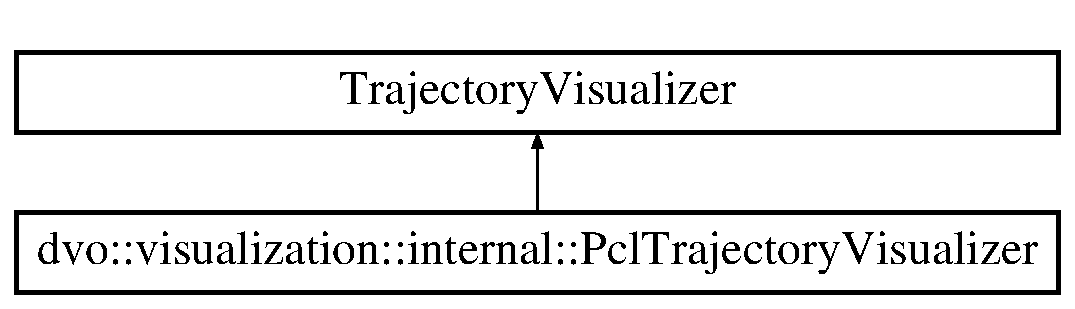
\includegraphics[height=2.000000cm]{classdvo_1_1visualization_1_1internal_1_1_pcl_trajectory_visualizer}
\end{center}
\end{figure}
\subsection*{Public Member Functions}
\begin{DoxyCompactItemize}
\item 
\mbox{\hyperlink{classdvo_1_1visualization_1_1internal_1_1_pcl_trajectory_visualizer_a666f91d73d3a6ae83444bcca62e36bec}{Pcl\+Trajectory\+Visualizer}} (std\+::string \&name)
\item 
virtual \mbox{\hyperlink{classdvo_1_1visualization_1_1_trajectory_visualizer}{Trajectory\+Visualizer}} \& \mbox{\hyperlink{classdvo_1_1visualization_1_1internal_1_1_pcl_trajectory_visualizer_aa174b5910657b2bfed45dfacd429a75a}{add}} (const Eigen\+::\+Affine3d \&pose)
\item 
void \mbox{\hyperlink{classdvo_1_1visualization_1_1internal_1_1_pcl_trajectory_visualizer_a16c8c79c3773408afba9ef57fcaea9e2}{update\+Visualizer}} (pcl\+::visualization\+::\+P\+C\+L\+Visualizer \&visualizer)
\end{DoxyCompactItemize}
\subsection*{Additional Inherited Members}


\subsection{Constructor \& Destructor Documentation}
\mbox{\Hypertarget{classdvo_1_1visualization_1_1internal_1_1_pcl_trajectory_visualizer_a666f91d73d3a6ae83444bcca62e36bec}\label{classdvo_1_1visualization_1_1internal_1_1_pcl_trajectory_visualizer_a666f91d73d3a6ae83444bcca62e36bec}} 
\index{dvo\+::visualization\+::internal\+::\+Pcl\+Trajectory\+Visualizer@{dvo\+::visualization\+::internal\+::\+Pcl\+Trajectory\+Visualizer}!Pcl\+Trajectory\+Visualizer@{Pcl\+Trajectory\+Visualizer}}
\index{Pcl\+Trajectory\+Visualizer@{Pcl\+Trajectory\+Visualizer}!dvo\+::visualization\+::internal\+::\+Pcl\+Trajectory\+Visualizer@{dvo\+::visualization\+::internal\+::\+Pcl\+Trajectory\+Visualizer}}
\subsubsection{\texorpdfstring{Pcl\+Trajectory\+Visualizer()}{PclTrajectoryVisualizer()}}
{\footnotesize\ttfamily dvo\+::visualization\+::internal\+::\+Pcl\+Trajectory\+Visualizer\+::\+Pcl\+Trajectory\+Visualizer (\begin{DoxyParamCaption}\item[{std\+::string \&}]{name }\end{DoxyParamCaption})\hspace{0.3cm}{\ttfamily [inline]}}



\subsection{Member Function Documentation}
\mbox{\Hypertarget{classdvo_1_1visualization_1_1internal_1_1_pcl_trajectory_visualizer_aa174b5910657b2bfed45dfacd429a75a}\label{classdvo_1_1visualization_1_1internal_1_1_pcl_trajectory_visualizer_aa174b5910657b2bfed45dfacd429a75a}} 
\index{dvo\+::visualization\+::internal\+::\+Pcl\+Trajectory\+Visualizer@{dvo\+::visualization\+::internal\+::\+Pcl\+Trajectory\+Visualizer}!add@{add}}
\index{add@{add}!dvo\+::visualization\+::internal\+::\+Pcl\+Trajectory\+Visualizer@{dvo\+::visualization\+::internal\+::\+Pcl\+Trajectory\+Visualizer}}
\subsubsection{\texorpdfstring{add()}{add()}}
{\footnotesize\ttfamily virtual \mbox{\hyperlink{classdvo_1_1visualization_1_1_trajectory_visualizer}{Trajectory\+Visualizer}}\& dvo\+::visualization\+::internal\+::\+Pcl\+Trajectory\+Visualizer\+::add (\begin{DoxyParamCaption}\item[{const Eigen\+::\+Affine3d \&}]{pose }\end{DoxyParamCaption})\hspace{0.3cm}{\ttfamily [inline]}, {\ttfamily [virtual]}}



Implements \mbox{\hyperlink{classdvo_1_1visualization_1_1_trajectory_visualizer_ac41106ae7e28c019b03f0aa210c6f0c1}{dvo\+::visualization\+::\+Trajectory\+Visualizer}}.

\mbox{\Hypertarget{classdvo_1_1visualization_1_1internal_1_1_pcl_trajectory_visualizer_a16c8c79c3773408afba9ef57fcaea9e2}\label{classdvo_1_1visualization_1_1internal_1_1_pcl_trajectory_visualizer_a16c8c79c3773408afba9ef57fcaea9e2}} 
\index{dvo\+::visualization\+::internal\+::\+Pcl\+Trajectory\+Visualizer@{dvo\+::visualization\+::internal\+::\+Pcl\+Trajectory\+Visualizer}!update\+Visualizer@{update\+Visualizer}}
\index{update\+Visualizer@{update\+Visualizer}!dvo\+::visualization\+::internal\+::\+Pcl\+Trajectory\+Visualizer@{dvo\+::visualization\+::internal\+::\+Pcl\+Trajectory\+Visualizer}}
\subsubsection{\texorpdfstring{update\+Visualizer()}{updateVisualizer()}}
{\footnotesize\ttfamily void dvo\+::visualization\+::internal\+::\+Pcl\+Trajectory\+Visualizer\+::update\+Visualizer (\begin{DoxyParamCaption}\item[{pcl\+::visualization\+::\+P\+C\+L\+Visualizer \&}]{visualizer }\end{DoxyParamCaption})\hspace{0.3cm}{\ttfamily [inline]}}



The documentation for this class was generated from the following file\+:\begin{DoxyCompactItemize}
\item 
dvo\+\_\+core/src/visualization/\mbox{\hyperlink{pcl__camera__trajetory__visualizer_8cpp}{pcl\+\_\+camera\+\_\+trajetory\+\_\+visualizer.\+cpp}}\end{DoxyCompactItemize}

\hypertarget{classdvo_1_1visualization_1_1internal_1_1_point_cloud_aggregator_impl}{}\section{dvo\+:\+:visualization\+:\+:internal\+:\+:Point\+Cloud\+Aggregator\+Impl Class Reference}
\label{classdvo_1_1visualization_1_1internal_1_1_point_cloud_aggregator_impl}\index{dvo\+::visualization\+::internal\+::\+Point\+Cloud\+Aggregator\+Impl@{dvo\+::visualization\+::internal\+::\+Point\+Cloud\+Aggregator\+Impl}}
\subsection*{Public Member Functions}
\begin{DoxyCompactItemize}
\item 
\mbox{\hyperlink{classdvo_1_1visualization_1_1internal_1_1_point_cloud_aggregator_impl_a6d3ae4b9c5a446fa954e159a2768d231}{Point\+Cloud\+Aggregator\+Impl}} ()
\item 
\mbox{\hyperlink{classdvo_1_1visualization_1_1internal_1_1_point_cloud_aggregator_impl_a4c02fb3f527603af8bb1bedb7ae45ea9}{$\sim$\+Point\+Cloud\+Aggregator\+Impl}} ()
\end{DoxyCompactItemize}
\subsection*{Public Attributes}
\begin{DoxyCompactItemize}
\item 
\mbox{\hyperlink{namespacedvo_1_1visualization_a6bfc209b639de1fc1fb54582af7292f7}{Point\+Cloud\+Map}} \mbox{\hyperlink{classdvo_1_1visualization_1_1internal_1_1_point_cloud_aggregator_impl_a0ea4be19b451e1d10c5d2b14c02e11e9}{clouds\+\_\+}}
\item 
boost\+::mutex \mbox{\hyperlink{classdvo_1_1visualization_1_1internal_1_1_point_cloud_aggregator_impl_a1b959ce567fa43e695eab5c33b56ab4f}{clouds\+\_\+mutex\+\_\+}}
\end{DoxyCompactItemize}


\subsection{Constructor \& Destructor Documentation}
\mbox{\Hypertarget{classdvo_1_1visualization_1_1internal_1_1_point_cloud_aggregator_impl_a6d3ae4b9c5a446fa954e159a2768d231}\label{classdvo_1_1visualization_1_1internal_1_1_point_cloud_aggregator_impl_a6d3ae4b9c5a446fa954e159a2768d231}} 
\index{dvo\+::visualization\+::internal\+::\+Point\+Cloud\+Aggregator\+Impl@{dvo\+::visualization\+::internal\+::\+Point\+Cloud\+Aggregator\+Impl}!Point\+Cloud\+Aggregator\+Impl@{Point\+Cloud\+Aggregator\+Impl}}
\index{Point\+Cloud\+Aggregator\+Impl@{Point\+Cloud\+Aggregator\+Impl}!dvo\+::visualization\+::internal\+::\+Point\+Cloud\+Aggregator\+Impl@{dvo\+::visualization\+::internal\+::\+Point\+Cloud\+Aggregator\+Impl}}
\subsubsection{\texorpdfstring{Point\+Cloud\+Aggregator\+Impl()}{PointCloudAggregatorImpl()}}
{\footnotesize\ttfamily dvo\+::visualization\+::internal\+::\+Point\+Cloud\+Aggregator\+Impl\+::\+Point\+Cloud\+Aggregator\+Impl (\begin{DoxyParamCaption}{ }\end{DoxyParamCaption})\hspace{0.3cm}{\ttfamily [inline]}}

\mbox{\Hypertarget{classdvo_1_1visualization_1_1internal_1_1_point_cloud_aggregator_impl_a4c02fb3f527603af8bb1bedb7ae45ea9}\label{classdvo_1_1visualization_1_1internal_1_1_point_cloud_aggregator_impl_a4c02fb3f527603af8bb1bedb7ae45ea9}} 
\index{dvo\+::visualization\+::internal\+::\+Point\+Cloud\+Aggregator\+Impl@{dvo\+::visualization\+::internal\+::\+Point\+Cloud\+Aggregator\+Impl}!````~Point\+Cloud\+Aggregator\+Impl@{$\sim$\+Point\+Cloud\+Aggregator\+Impl}}
\index{````~Point\+Cloud\+Aggregator\+Impl@{$\sim$\+Point\+Cloud\+Aggregator\+Impl}!dvo\+::visualization\+::internal\+::\+Point\+Cloud\+Aggregator\+Impl@{dvo\+::visualization\+::internal\+::\+Point\+Cloud\+Aggregator\+Impl}}
\subsubsection{\texorpdfstring{$\sim$\+Point\+Cloud\+Aggregator\+Impl()}{~PointCloudAggregatorImpl()}}
{\footnotesize\ttfamily dvo\+::visualization\+::internal\+::\+Point\+Cloud\+Aggregator\+Impl\+::$\sim$\+Point\+Cloud\+Aggregator\+Impl (\begin{DoxyParamCaption}{ }\end{DoxyParamCaption})\hspace{0.3cm}{\ttfamily [inline]}}



\subsection{Member Data Documentation}
\mbox{\Hypertarget{classdvo_1_1visualization_1_1internal_1_1_point_cloud_aggregator_impl_a0ea4be19b451e1d10c5d2b14c02e11e9}\label{classdvo_1_1visualization_1_1internal_1_1_point_cloud_aggregator_impl_a0ea4be19b451e1d10c5d2b14c02e11e9}} 
\index{dvo\+::visualization\+::internal\+::\+Point\+Cloud\+Aggregator\+Impl@{dvo\+::visualization\+::internal\+::\+Point\+Cloud\+Aggregator\+Impl}!clouds\+\_\+@{clouds\+\_\+}}
\index{clouds\+\_\+@{clouds\+\_\+}!dvo\+::visualization\+::internal\+::\+Point\+Cloud\+Aggregator\+Impl@{dvo\+::visualization\+::internal\+::\+Point\+Cloud\+Aggregator\+Impl}}
\subsubsection{\texorpdfstring{clouds\+\_\+}{clouds\_}}
{\footnotesize\ttfamily \mbox{\hyperlink{namespacedvo_1_1visualization_a6bfc209b639de1fc1fb54582af7292f7}{Point\+Cloud\+Map}} dvo\+::visualization\+::internal\+::\+Point\+Cloud\+Aggregator\+Impl\+::clouds\+\_\+}

\mbox{\Hypertarget{classdvo_1_1visualization_1_1internal_1_1_point_cloud_aggregator_impl_a1b959ce567fa43e695eab5c33b56ab4f}\label{classdvo_1_1visualization_1_1internal_1_1_point_cloud_aggregator_impl_a1b959ce567fa43e695eab5c33b56ab4f}} 
\index{dvo\+::visualization\+::internal\+::\+Point\+Cloud\+Aggregator\+Impl@{dvo\+::visualization\+::internal\+::\+Point\+Cloud\+Aggregator\+Impl}!clouds\+\_\+mutex\+\_\+@{clouds\+\_\+mutex\+\_\+}}
\index{clouds\+\_\+mutex\+\_\+@{clouds\+\_\+mutex\+\_\+}!dvo\+::visualization\+::internal\+::\+Point\+Cloud\+Aggregator\+Impl@{dvo\+::visualization\+::internal\+::\+Point\+Cloud\+Aggregator\+Impl}}
\subsubsection{\texorpdfstring{clouds\+\_\+mutex\+\_\+}{clouds\_mutex\_}}
{\footnotesize\ttfamily boost\+::mutex dvo\+::visualization\+::internal\+::\+Point\+Cloud\+Aggregator\+Impl\+::clouds\+\_\+mutex\+\_\+}



The documentation for this class was generated from the following file\+:\begin{DoxyCompactItemize}
\item 
visualization/\mbox{\hyperlink{point__cloud__aggregator_8cpp}{point\+\_\+cloud\+\_\+aggregator.\+cpp}}\end{DoxyCompactItemize}

\hypertarget{structdvo_1_1core_1_1_t_distribution_scale_reduction}{}\section{dvo\+:\+:core\+:\+:T\+Distribution\+Scale\+Reduction Struct Reference}
\label{structdvo_1_1core_1_1_t_distribution_scale_reduction}\index{dvo\+::core\+::\+T\+Distribution\+Scale\+Reduction@{dvo\+::core\+::\+T\+Distribution\+Scale\+Reduction}}
\subsection*{Public Member Functions}
\begin{DoxyCompactItemize}
\item 
\mbox{\hyperlink{structdvo_1_1core_1_1_t_distribution_scale_reduction_aa7e02d101f48cc6442918820908efb1c}{T\+Distribution\+Scale\+Reduction}} (const float $\ast$\mbox{\hyperlink{structdvo_1_1core_1_1_t_distribution_scale_reduction_a6259219785a8c3d0419af876182eea8f}{data}}, const float \mbox{\hyperlink{structdvo_1_1core_1_1_t_distribution_scale_reduction_af54018029273dd4a0fded86ace3a6527}{initial\+\_\+lambda}}, const float \mbox{\hyperlink{structdvo_1_1core_1_1_t_distribution_scale_reduction_a351c0ce2b6638b1e0ebd6992d7299feb}{dof}})
\item 
\mbox{\hyperlink{structdvo_1_1core_1_1_t_distribution_scale_reduction_a74f0bb1130ab1e03931cb173d9a0fff9}{T\+Distribution\+Scale\+Reduction}} (\mbox{\hyperlink{structdvo_1_1core_1_1_t_distribution_scale_reduction}{T\+Distribution\+Scale\+Reduction}} \&other, tbb\+::split)
\item 
void \mbox{\hyperlink{structdvo_1_1core_1_1_t_distribution_scale_reduction_a818757987df87f3eeae3b7a3bfda978d}{operator()}} (const tbb\+::blocked\+\_\+range$<$ size\+\_\+t $>$ \&r)
\item 
void \mbox{\hyperlink{structdvo_1_1core_1_1_t_distribution_scale_reduction_a50165f036a45706cd93e36e38a8b04a4}{join}} (\mbox{\hyperlink{structdvo_1_1core_1_1_t_distribution_scale_reduction}{T\+Distribution\+Scale\+Reduction}} \&other)
\end{DoxyCompactItemize}
\subsection*{Public Attributes}
\begin{DoxyCompactItemize}
\item 
const float $\ast$ \mbox{\hyperlink{structdvo_1_1core_1_1_t_distribution_scale_reduction_a6259219785a8c3d0419af876182eea8f}{data}}
\item 
const float \mbox{\hyperlink{structdvo_1_1core_1_1_t_distribution_scale_reduction_af54018029273dd4a0fded86ace3a6527}{initial\+\_\+lambda}}
\item 
const float \mbox{\hyperlink{structdvo_1_1core_1_1_t_distribution_scale_reduction_a351c0ce2b6638b1e0ebd6992d7299feb}{dof}}
\item 
float \mbox{\hyperlink{structdvo_1_1core_1_1_t_distribution_scale_reduction_a94c67a95846c5067b0305fd748d3c461}{lambda}}
\item 
float \mbox{\hyperlink{structdvo_1_1core_1_1_t_distribution_scale_reduction_a9935c3abdf8b53f63b42a3b7c2825bb1}{num}}
\end{DoxyCompactItemize}


\subsection{Constructor \& Destructor Documentation}
\mbox{\Hypertarget{structdvo_1_1core_1_1_t_distribution_scale_reduction_aa7e02d101f48cc6442918820908efb1c}\label{structdvo_1_1core_1_1_t_distribution_scale_reduction_aa7e02d101f48cc6442918820908efb1c}} 
\index{dvo\+::core\+::\+T\+Distribution\+Scale\+Reduction@{dvo\+::core\+::\+T\+Distribution\+Scale\+Reduction}!T\+Distribution\+Scale\+Reduction@{T\+Distribution\+Scale\+Reduction}}
\index{T\+Distribution\+Scale\+Reduction@{T\+Distribution\+Scale\+Reduction}!dvo\+::core\+::\+T\+Distribution\+Scale\+Reduction@{dvo\+::core\+::\+T\+Distribution\+Scale\+Reduction}}
\subsubsection{\texorpdfstring{T\+Distribution\+Scale\+Reduction()}{TDistributionScaleReduction()}\hspace{0.1cm}{\footnotesize\ttfamily [1/2]}}
{\footnotesize\ttfamily dvo\+::core\+::\+T\+Distribution\+Scale\+Reduction\+::\+T\+Distribution\+Scale\+Reduction (\begin{DoxyParamCaption}\item[{const float $\ast$}]{data,  }\item[{const float}]{initial\+\_\+lambda,  }\item[{const float}]{dof }\end{DoxyParamCaption})\hspace{0.3cm}{\ttfamily [inline]}}

\mbox{\Hypertarget{structdvo_1_1core_1_1_t_distribution_scale_reduction_a74f0bb1130ab1e03931cb173d9a0fff9}\label{structdvo_1_1core_1_1_t_distribution_scale_reduction_a74f0bb1130ab1e03931cb173d9a0fff9}} 
\index{dvo\+::core\+::\+T\+Distribution\+Scale\+Reduction@{dvo\+::core\+::\+T\+Distribution\+Scale\+Reduction}!T\+Distribution\+Scale\+Reduction@{T\+Distribution\+Scale\+Reduction}}
\index{T\+Distribution\+Scale\+Reduction@{T\+Distribution\+Scale\+Reduction}!dvo\+::core\+::\+T\+Distribution\+Scale\+Reduction@{dvo\+::core\+::\+T\+Distribution\+Scale\+Reduction}}
\subsubsection{\texorpdfstring{T\+Distribution\+Scale\+Reduction()}{TDistributionScaleReduction()}\hspace{0.1cm}{\footnotesize\ttfamily [2/2]}}
{\footnotesize\ttfamily dvo\+::core\+::\+T\+Distribution\+Scale\+Reduction\+::\+T\+Distribution\+Scale\+Reduction (\begin{DoxyParamCaption}\item[{\mbox{\hyperlink{structdvo_1_1core_1_1_t_distribution_scale_reduction}{T\+Distribution\+Scale\+Reduction}} \&}]{other,  }\item[{tbb\+::split}]{ }\end{DoxyParamCaption})\hspace{0.3cm}{\ttfamily [inline]}}



\subsection{Member Function Documentation}
\mbox{\Hypertarget{structdvo_1_1core_1_1_t_distribution_scale_reduction_a50165f036a45706cd93e36e38a8b04a4}\label{structdvo_1_1core_1_1_t_distribution_scale_reduction_a50165f036a45706cd93e36e38a8b04a4}} 
\index{dvo\+::core\+::\+T\+Distribution\+Scale\+Reduction@{dvo\+::core\+::\+T\+Distribution\+Scale\+Reduction}!join@{join}}
\index{join@{join}!dvo\+::core\+::\+T\+Distribution\+Scale\+Reduction@{dvo\+::core\+::\+T\+Distribution\+Scale\+Reduction}}
\subsubsection{\texorpdfstring{join()}{join()}}
{\footnotesize\ttfamily void dvo\+::core\+::\+T\+Distribution\+Scale\+Reduction\+::join (\begin{DoxyParamCaption}\item[{\mbox{\hyperlink{structdvo_1_1core_1_1_t_distribution_scale_reduction}{T\+Distribution\+Scale\+Reduction}} \&}]{other }\end{DoxyParamCaption})\hspace{0.3cm}{\ttfamily [inline]}}

\mbox{\Hypertarget{structdvo_1_1core_1_1_t_distribution_scale_reduction_a818757987df87f3eeae3b7a3bfda978d}\label{structdvo_1_1core_1_1_t_distribution_scale_reduction_a818757987df87f3eeae3b7a3bfda978d}} 
\index{dvo\+::core\+::\+T\+Distribution\+Scale\+Reduction@{dvo\+::core\+::\+T\+Distribution\+Scale\+Reduction}!operator()@{operator()}}
\index{operator()@{operator()}!dvo\+::core\+::\+T\+Distribution\+Scale\+Reduction@{dvo\+::core\+::\+T\+Distribution\+Scale\+Reduction}}
\subsubsection{\texorpdfstring{operator()()}{operator()()}}
{\footnotesize\ttfamily void dvo\+::core\+::\+T\+Distribution\+Scale\+Reduction\+::operator() (\begin{DoxyParamCaption}\item[{const tbb\+::blocked\+\_\+range$<$ size\+\_\+t $>$ \&}]{r }\end{DoxyParamCaption})\hspace{0.3cm}{\ttfamily [inline]}}



\subsection{Member Data Documentation}
\mbox{\Hypertarget{structdvo_1_1core_1_1_t_distribution_scale_reduction_a6259219785a8c3d0419af876182eea8f}\label{structdvo_1_1core_1_1_t_distribution_scale_reduction_a6259219785a8c3d0419af876182eea8f}} 
\index{dvo\+::core\+::\+T\+Distribution\+Scale\+Reduction@{dvo\+::core\+::\+T\+Distribution\+Scale\+Reduction}!data@{data}}
\index{data@{data}!dvo\+::core\+::\+T\+Distribution\+Scale\+Reduction@{dvo\+::core\+::\+T\+Distribution\+Scale\+Reduction}}
\subsubsection{\texorpdfstring{data}{data}}
{\footnotesize\ttfamily const float$\ast$ dvo\+::core\+::\+T\+Distribution\+Scale\+Reduction\+::data}

\mbox{\Hypertarget{structdvo_1_1core_1_1_t_distribution_scale_reduction_a351c0ce2b6638b1e0ebd6992d7299feb}\label{structdvo_1_1core_1_1_t_distribution_scale_reduction_a351c0ce2b6638b1e0ebd6992d7299feb}} 
\index{dvo\+::core\+::\+T\+Distribution\+Scale\+Reduction@{dvo\+::core\+::\+T\+Distribution\+Scale\+Reduction}!dof@{dof}}
\index{dof@{dof}!dvo\+::core\+::\+T\+Distribution\+Scale\+Reduction@{dvo\+::core\+::\+T\+Distribution\+Scale\+Reduction}}
\subsubsection{\texorpdfstring{dof}{dof}}
{\footnotesize\ttfamily const float dvo\+::core\+::\+T\+Distribution\+Scale\+Reduction\+::dof}

\mbox{\Hypertarget{structdvo_1_1core_1_1_t_distribution_scale_reduction_af54018029273dd4a0fded86ace3a6527}\label{structdvo_1_1core_1_1_t_distribution_scale_reduction_af54018029273dd4a0fded86ace3a6527}} 
\index{dvo\+::core\+::\+T\+Distribution\+Scale\+Reduction@{dvo\+::core\+::\+T\+Distribution\+Scale\+Reduction}!initial\+\_\+lambda@{initial\+\_\+lambda}}
\index{initial\+\_\+lambda@{initial\+\_\+lambda}!dvo\+::core\+::\+T\+Distribution\+Scale\+Reduction@{dvo\+::core\+::\+T\+Distribution\+Scale\+Reduction}}
\subsubsection{\texorpdfstring{initial\+\_\+lambda}{initial\_lambda}}
{\footnotesize\ttfamily const float dvo\+::core\+::\+T\+Distribution\+Scale\+Reduction\+::initial\+\_\+lambda}

\mbox{\Hypertarget{structdvo_1_1core_1_1_t_distribution_scale_reduction_a94c67a95846c5067b0305fd748d3c461}\label{structdvo_1_1core_1_1_t_distribution_scale_reduction_a94c67a95846c5067b0305fd748d3c461}} 
\index{dvo\+::core\+::\+T\+Distribution\+Scale\+Reduction@{dvo\+::core\+::\+T\+Distribution\+Scale\+Reduction}!lambda@{lambda}}
\index{lambda@{lambda}!dvo\+::core\+::\+T\+Distribution\+Scale\+Reduction@{dvo\+::core\+::\+T\+Distribution\+Scale\+Reduction}}
\subsubsection{\texorpdfstring{lambda}{lambda}}
{\footnotesize\ttfamily float dvo\+::core\+::\+T\+Distribution\+Scale\+Reduction\+::lambda}

\mbox{\Hypertarget{structdvo_1_1core_1_1_t_distribution_scale_reduction_a9935c3abdf8b53f63b42a3b7c2825bb1}\label{structdvo_1_1core_1_1_t_distribution_scale_reduction_a9935c3abdf8b53f63b42a3b7c2825bb1}} 
\index{dvo\+::core\+::\+T\+Distribution\+Scale\+Reduction@{dvo\+::core\+::\+T\+Distribution\+Scale\+Reduction}!num@{num}}
\index{num@{num}!dvo\+::core\+::\+T\+Distribution\+Scale\+Reduction@{dvo\+::core\+::\+T\+Distribution\+Scale\+Reduction}}
\subsubsection{\texorpdfstring{num}{num}}
{\footnotesize\ttfamily float dvo\+::core\+::\+T\+Distribution\+Scale\+Reduction\+::num}



The documentation for this struct was generated from the following file\+:\begin{DoxyCompactItemize}
\item 
core/\mbox{\hyperlink{weight__calculation_8cpp}{weight\+\_\+calculation.\+cpp}}\end{DoxyCompactItemize}

\hypertarget{classdvo_1_1visualization_1_1_visualizer_impl}{}\section{dvo\+:\+:visualization\+:\+:Visualizer\+Impl Class Reference}
\label{classdvo_1_1visualization_1_1_visualizer_impl}\index{dvo\+::visualization\+::\+Visualizer\+Impl@{dvo\+::visualization\+::\+Visualizer\+Impl}}
\subsection*{Classes}
\begin{DoxyCompactItemize}
\item 
struct \mbox{\hyperlink{structdvo_1_1visualization_1_1_visualizer_impl_1_1_create_histogram_func}{Create\+Histogram\+Func}}
\item 
struct \mbox{\hyperlink{structdvo_1_1visualization_1_1_visualizer_impl_1_1_named_image}{Named\+Image}}
\end{DoxyCompactItemize}
\subsection*{Public Types}
\begin{DoxyCompactItemize}
\item 
typedef std\+::map$<$ std\+::string, cv\+::\+Size $>$ \mbox{\hyperlink{classdvo_1_1visualization_1_1_visualizer_impl_a06868ed07bf4f004fd6446e92f4cda7a}{Name\+Size\+Map}}
\item 
typedef std\+::map$<$ std\+::string, int $>$ \mbox{\hyperlink{classdvo_1_1visualization_1_1_visualizer_impl_ad1bbf4cb3b9cfbb104f6a568c605119e}{Name\+Sequence\+Map}}
\end{DoxyCompactItemize}
\subsection*{Public Member Functions}
\begin{DoxyCompactItemize}
\item 
\mbox{\hyperlink{classdvo_1_1visualization_1_1_visualizer_impl_ac9bacd20873b2204c007d8ae897dd793}{Visualizer\+Impl}} ()
\item 
\mbox{\hyperlink{classdvo_1_1visualization_1_1_visualizer_impl_ab2671b8d7b177f4833e308034eeee6a5}{$\sim$\+Visualizer\+Impl}} ()
\item 
void \mbox{\hyperlink{classdvo_1_1visualization_1_1_visualizer_impl_a2076b6b3056314a8bacacdf2fbbfff71}{show}} (std\+::string \&name, const cv\+::\+Mat\+Expr \&img, Visualizer\+::\+Image\+Modifier modifier)
\item 
void \mbox{\hyperlink{classdvo_1_1visualization_1_1_visualizer_impl_a3afe414ca4a899c77458a1a0f1139dbc}{show\+Histogram}} (std\+::string \&name, const cv\+::\+Mat \&img, float binsize, float min, float max)
\item 
void \mbox{\hyperlink{classdvo_1_1visualization_1_1_visualizer_impl_ab7dc97f7e3e3444fb5337fd0e393a237}{internal\+Show}} (std\+::string \&name, const cv\+::\+Mat\+Expr \&img, Visualizer\+::\+Image\+Modifier modifier=Visualizer\+::\+Image\+Modifier())
\item 
bool \mbox{\hyperlink{classdvo_1_1visualization_1_1_visualizer_impl_a0401f138611fc10aa4c8ef3bfb37d02f}{check\+Image\+Size}} (std\+::string \&name, const cv\+::\+Mat \&img)
\item 
void \mbox{\hyperlink{classdvo_1_1visualization_1_1_visualizer_impl_acc30618615be0c6b9d54959a1beaf5e7}{vis\+Worker}} ()
\item 
void \mbox{\hyperlink{classdvo_1_1visualization_1_1_visualizer_impl_aaa9bdf78dde7df4c88fa61c05bfb13bd}{histogram\+Worker}} ()
\end{DoxyCompactItemize}
\subsection*{Public Attributes}
\begin{DoxyCompactItemize}
\item 
bool \mbox{\hyperlink{classdvo_1_1visualization_1_1_visualizer_impl_ae8de60588232e3a67c19e840f8363e2c}{external\+\_\+wait\+\_\+}}
\item 
bool \mbox{\hyperlink{classdvo_1_1visualization_1_1_visualizer_impl_a9142982073b53d888e0533ccf552d903}{save\+\_\+}}
\end{DoxyCompactItemize}


\subsection{Member Typedef Documentation}
\mbox{\Hypertarget{classdvo_1_1visualization_1_1_visualizer_impl_ad1bbf4cb3b9cfbb104f6a568c605119e}\label{classdvo_1_1visualization_1_1_visualizer_impl_ad1bbf4cb3b9cfbb104f6a568c605119e}} 
\index{dvo\+::visualization\+::\+Visualizer\+Impl@{dvo\+::visualization\+::\+Visualizer\+Impl}!Name\+Sequence\+Map@{Name\+Sequence\+Map}}
\index{Name\+Sequence\+Map@{Name\+Sequence\+Map}!dvo\+::visualization\+::\+Visualizer\+Impl@{dvo\+::visualization\+::\+Visualizer\+Impl}}
\subsubsection{\texorpdfstring{Name\+Sequence\+Map}{NameSequenceMap}}
{\footnotesize\ttfamily typedef std\+::map$<$std\+::string, int$>$ \mbox{\hyperlink{classdvo_1_1visualization_1_1_visualizer_impl_ad1bbf4cb3b9cfbb104f6a568c605119e}{dvo\+::visualization\+::\+Visualizer\+Impl\+::\+Name\+Sequence\+Map}}}

\mbox{\Hypertarget{classdvo_1_1visualization_1_1_visualizer_impl_a06868ed07bf4f004fd6446e92f4cda7a}\label{classdvo_1_1visualization_1_1_visualizer_impl_a06868ed07bf4f004fd6446e92f4cda7a}} 
\index{dvo\+::visualization\+::\+Visualizer\+Impl@{dvo\+::visualization\+::\+Visualizer\+Impl}!Name\+Size\+Map@{Name\+Size\+Map}}
\index{Name\+Size\+Map@{Name\+Size\+Map}!dvo\+::visualization\+::\+Visualizer\+Impl@{dvo\+::visualization\+::\+Visualizer\+Impl}}
\subsubsection{\texorpdfstring{Name\+Size\+Map}{NameSizeMap}}
{\footnotesize\ttfamily typedef std\+::map$<$std\+::string, cv\+::\+Size$>$ \mbox{\hyperlink{classdvo_1_1visualization_1_1_visualizer_impl_a06868ed07bf4f004fd6446e92f4cda7a}{dvo\+::visualization\+::\+Visualizer\+Impl\+::\+Name\+Size\+Map}}}



\subsection{Constructor \& Destructor Documentation}
\mbox{\Hypertarget{classdvo_1_1visualization_1_1_visualizer_impl_ac9bacd20873b2204c007d8ae897dd793}\label{classdvo_1_1visualization_1_1_visualizer_impl_ac9bacd20873b2204c007d8ae897dd793}} 
\index{dvo\+::visualization\+::\+Visualizer\+Impl@{dvo\+::visualization\+::\+Visualizer\+Impl}!Visualizer\+Impl@{Visualizer\+Impl}}
\index{Visualizer\+Impl@{Visualizer\+Impl}!dvo\+::visualization\+::\+Visualizer\+Impl@{dvo\+::visualization\+::\+Visualizer\+Impl}}
\subsubsection{\texorpdfstring{Visualizer\+Impl()}{VisualizerImpl()}}
{\footnotesize\ttfamily dvo\+::visualization\+::\+Visualizer\+Impl\+::\+Visualizer\+Impl (\begin{DoxyParamCaption}{ }\end{DoxyParamCaption})\hspace{0.3cm}{\ttfamily [inline]}}

\mbox{\Hypertarget{classdvo_1_1visualization_1_1_visualizer_impl_ab2671b8d7b177f4833e308034eeee6a5}\label{classdvo_1_1visualization_1_1_visualizer_impl_ab2671b8d7b177f4833e308034eeee6a5}} 
\index{dvo\+::visualization\+::\+Visualizer\+Impl@{dvo\+::visualization\+::\+Visualizer\+Impl}!````~Visualizer\+Impl@{$\sim$\+Visualizer\+Impl}}
\index{````~Visualizer\+Impl@{$\sim$\+Visualizer\+Impl}!dvo\+::visualization\+::\+Visualizer\+Impl@{dvo\+::visualization\+::\+Visualizer\+Impl}}
\subsubsection{\texorpdfstring{$\sim$\+Visualizer\+Impl()}{~VisualizerImpl()}}
{\footnotesize\ttfamily dvo\+::visualization\+::\+Visualizer\+Impl\+::$\sim$\+Visualizer\+Impl (\begin{DoxyParamCaption}{ }\end{DoxyParamCaption})\hspace{0.3cm}{\ttfamily [inline]}}



\subsection{Member Function Documentation}
\mbox{\Hypertarget{classdvo_1_1visualization_1_1_visualizer_impl_a0401f138611fc10aa4c8ef3bfb37d02f}\label{classdvo_1_1visualization_1_1_visualizer_impl_a0401f138611fc10aa4c8ef3bfb37d02f}} 
\index{dvo\+::visualization\+::\+Visualizer\+Impl@{dvo\+::visualization\+::\+Visualizer\+Impl}!check\+Image\+Size@{check\+Image\+Size}}
\index{check\+Image\+Size@{check\+Image\+Size}!dvo\+::visualization\+::\+Visualizer\+Impl@{dvo\+::visualization\+::\+Visualizer\+Impl}}
\subsubsection{\texorpdfstring{check\+Image\+Size()}{checkImageSize()}}
{\footnotesize\ttfamily bool dvo\+::visualization\+::\+Visualizer\+Impl\+::check\+Image\+Size (\begin{DoxyParamCaption}\item[{std\+::string \&}]{name,  }\item[{const cv\+::\+Mat \&}]{img }\end{DoxyParamCaption})\hspace{0.3cm}{\ttfamily [inline]}}

\mbox{\Hypertarget{classdvo_1_1visualization_1_1_visualizer_impl_aaa9bdf78dde7df4c88fa61c05bfb13bd}\label{classdvo_1_1visualization_1_1_visualizer_impl_aaa9bdf78dde7df4c88fa61c05bfb13bd}} 
\index{dvo\+::visualization\+::\+Visualizer\+Impl@{dvo\+::visualization\+::\+Visualizer\+Impl}!histogram\+Worker@{histogram\+Worker}}
\index{histogram\+Worker@{histogram\+Worker}!dvo\+::visualization\+::\+Visualizer\+Impl@{dvo\+::visualization\+::\+Visualizer\+Impl}}
\subsubsection{\texorpdfstring{histogram\+Worker()}{histogramWorker()}}
{\footnotesize\ttfamily void dvo\+::visualization\+::\+Visualizer\+Impl\+::histogram\+Worker (\begin{DoxyParamCaption}{ }\end{DoxyParamCaption})\hspace{0.3cm}{\ttfamily [inline]}}

\mbox{\Hypertarget{classdvo_1_1visualization_1_1_visualizer_impl_ab7dc97f7e3e3444fb5337fd0e393a237}\label{classdvo_1_1visualization_1_1_visualizer_impl_ab7dc97f7e3e3444fb5337fd0e393a237}} 
\index{dvo\+::visualization\+::\+Visualizer\+Impl@{dvo\+::visualization\+::\+Visualizer\+Impl}!internal\+Show@{internal\+Show}}
\index{internal\+Show@{internal\+Show}!dvo\+::visualization\+::\+Visualizer\+Impl@{dvo\+::visualization\+::\+Visualizer\+Impl}}
\subsubsection{\texorpdfstring{internal\+Show()}{internalShow()}}
{\footnotesize\ttfamily void dvo\+::visualization\+::\+Visualizer\+Impl\+::internal\+Show (\begin{DoxyParamCaption}\item[{std\+::string \&}]{name,  }\item[{const cv\+::\+Mat\+Expr \&}]{img,  }\item[{Visualizer\+::\+Image\+Modifier}]{modifier = {\ttfamily Visualizer\+:\+:ImageModifier()} }\end{DoxyParamCaption})\hspace{0.3cm}{\ttfamily [inline]}}

\mbox{\Hypertarget{classdvo_1_1visualization_1_1_visualizer_impl_a2076b6b3056314a8bacacdf2fbbfff71}\label{classdvo_1_1visualization_1_1_visualizer_impl_a2076b6b3056314a8bacacdf2fbbfff71}} 
\index{dvo\+::visualization\+::\+Visualizer\+Impl@{dvo\+::visualization\+::\+Visualizer\+Impl}!show@{show}}
\index{show@{show}!dvo\+::visualization\+::\+Visualizer\+Impl@{dvo\+::visualization\+::\+Visualizer\+Impl}}
\subsubsection{\texorpdfstring{show()}{show()}}
{\footnotesize\ttfamily void dvo\+::visualization\+::\+Visualizer\+Impl\+::show (\begin{DoxyParamCaption}\item[{std\+::string \&}]{name,  }\item[{const cv\+::\+Mat\+Expr \&}]{img,  }\item[{Visualizer\+::\+Image\+Modifier}]{modifier }\end{DoxyParamCaption})\hspace{0.3cm}{\ttfamily [inline]}}

\mbox{\Hypertarget{classdvo_1_1visualization_1_1_visualizer_impl_a3afe414ca4a899c77458a1a0f1139dbc}\label{classdvo_1_1visualization_1_1_visualizer_impl_a3afe414ca4a899c77458a1a0f1139dbc}} 
\index{dvo\+::visualization\+::\+Visualizer\+Impl@{dvo\+::visualization\+::\+Visualizer\+Impl}!show\+Histogram@{show\+Histogram}}
\index{show\+Histogram@{show\+Histogram}!dvo\+::visualization\+::\+Visualizer\+Impl@{dvo\+::visualization\+::\+Visualizer\+Impl}}
\subsubsection{\texorpdfstring{show\+Histogram()}{showHistogram()}}
{\footnotesize\ttfamily void dvo\+::visualization\+::\+Visualizer\+Impl\+::show\+Histogram (\begin{DoxyParamCaption}\item[{std\+::string \&}]{name,  }\item[{const cv\+::\+Mat \&}]{img,  }\item[{float}]{binsize,  }\item[{float}]{min,  }\item[{float}]{max }\end{DoxyParamCaption})\hspace{0.3cm}{\ttfamily [inline]}}

\mbox{\Hypertarget{classdvo_1_1visualization_1_1_visualizer_impl_acc30618615be0c6b9d54959a1beaf5e7}\label{classdvo_1_1visualization_1_1_visualizer_impl_acc30618615be0c6b9d54959a1beaf5e7}} 
\index{dvo\+::visualization\+::\+Visualizer\+Impl@{dvo\+::visualization\+::\+Visualizer\+Impl}!vis\+Worker@{vis\+Worker}}
\index{vis\+Worker@{vis\+Worker}!dvo\+::visualization\+::\+Visualizer\+Impl@{dvo\+::visualization\+::\+Visualizer\+Impl}}
\subsubsection{\texorpdfstring{vis\+Worker()}{visWorker()}}
{\footnotesize\ttfamily void dvo\+::visualization\+::\+Visualizer\+Impl\+::vis\+Worker (\begin{DoxyParamCaption}{ }\end{DoxyParamCaption})\hspace{0.3cm}{\ttfamily [inline]}}



\subsection{Member Data Documentation}
\mbox{\Hypertarget{classdvo_1_1visualization_1_1_visualizer_impl_ae8de60588232e3a67c19e840f8363e2c}\label{classdvo_1_1visualization_1_1_visualizer_impl_ae8de60588232e3a67c19e840f8363e2c}} 
\index{dvo\+::visualization\+::\+Visualizer\+Impl@{dvo\+::visualization\+::\+Visualizer\+Impl}!external\+\_\+wait\+\_\+@{external\+\_\+wait\+\_\+}}
\index{external\+\_\+wait\+\_\+@{external\+\_\+wait\+\_\+}!dvo\+::visualization\+::\+Visualizer\+Impl@{dvo\+::visualization\+::\+Visualizer\+Impl}}
\subsubsection{\texorpdfstring{external\+\_\+wait\+\_\+}{external\_wait\_}}
{\footnotesize\ttfamily bool dvo\+::visualization\+::\+Visualizer\+Impl\+::external\+\_\+wait\+\_\+}

\mbox{\Hypertarget{classdvo_1_1visualization_1_1_visualizer_impl_a9142982073b53d888e0533ccf552d903}\label{classdvo_1_1visualization_1_1_visualizer_impl_a9142982073b53d888e0533ccf552d903}} 
\index{dvo\+::visualization\+::\+Visualizer\+Impl@{dvo\+::visualization\+::\+Visualizer\+Impl}!save\+\_\+@{save\+\_\+}}
\index{save\+\_\+@{save\+\_\+}!dvo\+::visualization\+::\+Visualizer\+Impl@{dvo\+::visualization\+::\+Visualizer\+Impl}}
\subsubsection{\texorpdfstring{save\+\_\+}{save\_}}
{\footnotesize\ttfamily bool dvo\+::visualization\+::\+Visualizer\+Impl\+::save\+\_\+}



The documentation for this class was generated from the following file\+:\begin{DoxyCompactItemize}
\item 
visualization/\mbox{\hyperlink{visualizer_8cpp}{visualizer.\+cpp}}\end{DoxyCompactItemize}

\chapter{File Documentation}
\hypertarget{interpolation_8cpp}{}\section{core/interpolation.cpp File Reference}
\label{interpolation_8cpp}\index{core/interpolation.\+cpp@{core/interpolation.\+cpp}}
{\ttfamily \#include $<$dvo/core/interpolation.\+h$>$}\newline
\subsection*{Namespaces}
\begin{DoxyCompactItemize}
\item 
 \mbox{\hyperlink{namespacedvo}{dvo}}
\item 
 \mbox{\hyperlink{namespacedvo_1_1core}{dvo\+::core}}
\end{DoxyCompactItemize}

\hypertarget{intrinsic__matrix_8cpp}{}\section{dvo\+\_\+core/src/core/intrinsic\+\_\+matrix.cpp File Reference}
\label{intrinsic__matrix_8cpp}\index{dvo\+\_\+core/src/core/intrinsic\+\_\+matrix.\+cpp@{dvo\+\_\+core/src/core/intrinsic\+\_\+matrix.\+cpp}}
{\ttfamily \#include $<$dvo/core/intrinsic\+\_\+matrix.\+h$>$}\newline
{\ttfamily \#include $<$boost/unordered\+\_\+map.\+hpp$>$}\newline
\subsection*{Namespaces}
\begin{DoxyCompactItemize}
\item 
 \mbox{\hyperlink{namespacedvo}{dvo}}
\item 
 \mbox{\hyperlink{namespacedvo_1_1core}{dvo\+::core}}
\end{DoxyCompactItemize}

\hypertarget{least__squares_8cpp}{}\section{core/least\+\_\+squares.cpp File Reference}
\label{least__squares_8cpp}\index{core/least\+\_\+squares.\+cpp@{core/least\+\_\+squares.\+cpp}}
{\ttfamily \#include $<$dvo/core/least\+\_\+squares.\+h$>$}\newline
{\ttfamily \#include $<$Eigen/\+Cholesky$>$}\newline
{\ttfamily \#include $<$Eigen/\+Eigenvalues$>$}\newline
{\ttfamily \#include $<$Eigen/\+S\+VD$>$}\newline
{\ttfamily \#include $<$dvo/core/math\+\_\+sse.\+h$>$}\newline

\hypertarget{math__sse_8cpp}{}\section{core/math\+\_\+sse.cpp File Reference}
\label{math__sse_8cpp}\index{core/math\+\_\+sse.\+cpp@{core/math\+\_\+sse.\+cpp}}
{\ttfamily \#include $<$dvo/core/math\+\_\+sse.\+h$>$}\newline
{\ttfamily \#include $<$immintrin.\+h$>$}\newline
{\ttfamily \#include $<$pmmintrin.\+h$>$}\newline
\subsection*{Namespaces}
\begin{DoxyCompactItemize}
\item 
 \mbox{\hyperlink{namespacedvo}{dvo}}
\item 
 \mbox{\hyperlink{namespacedvo_1_1core}{dvo\+::core}}
\end{DoxyCompactItemize}

\hypertarget{rgbd__image_8cpp}{}\section{dvo\+\_\+core/src/core/rgbd\+\_\+image.cpp File Reference}
\label{rgbd__image_8cpp}\index{dvo\+\_\+core/src/core/rgbd\+\_\+image.\+cpp@{dvo\+\_\+core/src/core/rgbd\+\_\+image.\+cpp}}
{\ttfamily \#include $<$dvo/core/rgbd\+\_\+image.\+h$>$}\newline
{\ttfamily \#include $<$assert.\+h$>$}\newline
{\ttfamily \#include $<$boost/unordered\+\_\+map.\+hpp$>$}\newline
{\ttfamily \#include $<$dvo/core/interpolation.\+h$>$}\newline
\subsection*{Namespaces}
\begin{DoxyCompactItemize}
\item 
 \mbox{\hyperlink{namespacedvo}{dvo}}
\item 
 \mbox{\hyperlink{namespacedvo_1_1core}{dvo\+::core}}
\end{DoxyCompactItemize}

\hypertarget{rgbd__image__sse_8cpp}{}\section{dvo\+\_\+core/src/core/rgbd\+\_\+image\+\_\+sse.cpp File Reference}
\label{rgbd__image__sse_8cpp}\index{dvo\+\_\+core/src/core/rgbd\+\_\+image\+\_\+sse.\+cpp@{dvo\+\_\+core/src/core/rgbd\+\_\+image\+\_\+sse.\+cpp}}
{\ttfamily \#include $<$dvo/core/datatypes.\+h$>$}\newline
{\ttfamily \#include $<$dvo/core/rgbd\+\_\+image.\+h$>$}\newline
{\ttfamily \#include $<$dvo/core/interpolation.\+h$>$}\newline
{\ttfamily \#include $<$immintrin.\+h$>$}\newline
{\ttfamily \#include $<$pmmintrin.\+h$>$}\newline
\subsection*{Namespaces}
\begin{DoxyCompactItemize}
\item 
 \mbox{\hyperlink{namespacedvo}{dvo}}
\item 
 \mbox{\hyperlink{namespacedvo_1_1core}{dvo\+::core}}
\end{DoxyCompactItemize}
\subsection*{Macros}
\begin{DoxyCompactItemize}
\item 
\#define \mbox{\hyperlink{rgbd__image__sse_8cpp_ae4ff5a07c6ff43ed11a3887ef7d524f2}{A\+L\+I\+GN}}~\+\_\+\+\_\+attribute\+\_\+\+\_\+((\+\_\+\+\_\+aligned\+\_\+\+\_\+(16)))
\end{DoxyCompactItemize}


\subsection{Macro Definition Documentation}
\mbox{\Hypertarget{rgbd__image__sse_8cpp_ae4ff5a07c6ff43ed11a3887ef7d524f2}\label{rgbd__image__sse_8cpp_ae4ff5a07c6ff43ed11a3887ef7d524f2}} 
\index{rgbd\+\_\+image\+\_\+sse.\+cpp@{rgbd\+\_\+image\+\_\+sse.\+cpp}!A\+L\+I\+GN@{A\+L\+I\+GN}}
\index{A\+L\+I\+GN@{A\+L\+I\+GN}!rgbd\+\_\+image\+\_\+sse.\+cpp@{rgbd\+\_\+image\+\_\+sse.\+cpp}}
\subsubsection{\texorpdfstring{A\+L\+I\+GN}{ALIGN}}
{\footnotesize\ttfamily \#define A\+L\+I\+GN~\+\_\+\+\_\+attribute\+\_\+\+\_\+((\+\_\+\+\_\+aligned\+\_\+\+\_\+(16)))}

This file is part of dvo.

Copyright 2012 Christian Kerl \href{mailto:christian.kerl@in.tum.de}{\tt christian.\+kerl@in.\+tum.\+de} (Technical University of Munich) For more information see \href{http://vision.in.tum.de/data/software/dvo}{\tt http\+://vision.\+in.\+tum.\+de/data/software/dvo}.

dvo is free software\+: you can redistribute it and/or modify it under the terms of the G\+NU General Public License as published by the Free Software Foundation, either version 3 of the License, or (at your option) any later version.

dvo is distributed in the hope that it will be useful, but W\+I\+T\+H\+O\+UT A\+NY W\+A\+R\+R\+A\+N\+TY; without even the implied warranty of M\+E\+R\+C\+H\+A\+N\+T\+A\+B\+I\+L\+I\+TY or F\+I\+T\+N\+E\+SS F\+OR A P\+A\+R\+T\+I\+C\+U\+L\+AR P\+U\+R\+P\+O\+SE. See the G\+NU General Public License for more details.

You should have received a copy of the G\+NU General Public License along with dvo. If not, see \href{http://www.gnu.org/licenses/}{\tt http\+://www.\+gnu.\+org/licenses/}. 
\hypertarget{surface__pyramid_8cpp}{}\section{dvo\+\_\+core/src/core/surface\+\_\+pyramid.cpp File Reference}
\label{surface__pyramid_8cpp}\index{dvo\+\_\+core/src/core/surface\+\_\+pyramid.\+cpp@{dvo\+\_\+core/src/core/surface\+\_\+pyramid.\+cpp}}
{\ttfamily \#include $<$dvo/core/surface\+\_\+pyramid.\+h$>$}\newline
{\ttfamily \#include $<$iostream$>$}\newline
\subsection*{Namespaces}
\begin{DoxyCompactItemize}
\item 
 \mbox{\hyperlink{namespacedvo}{dvo}}
\item 
 \mbox{\hyperlink{namespacedvo_1_1core}{dvo\+::core}}
\end{DoxyCompactItemize}

\hypertarget{weight__calculation_8cpp}{}\section{core/weight\+\_\+calculation.cpp File Reference}
\label{weight__calculation_8cpp}\index{core/weight\+\_\+calculation.\+cpp@{core/weight\+\_\+calculation.\+cpp}}
{\ttfamily \#include $<$tbb/parallel\+\_\+reduce.\+h$>$}\newline
{\ttfamily \#include $<$tbb/blocked\+\_\+range.\+h$>$}\newline
{\ttfamily \#include $<$dvo/core/weight\+\_\+calculation.\+h$>$}\newline
{\ttfamily \#include $<$dvo/util/histogram.\+h$>$}\newline
{\ttfamily \#include $<$dvo/visualization/visualizer.\+h$>$}\newline
\subsection*{Classes}
\begin{DoxyCompactItemize}
\item 
struct \mbox{\hyperlink{structdvo_1_1core_1_1_t_distribution_scale_reduction}{dvo\+::core\+::\+T\+Distribution\+Scale\+Reduction}}
\end{DoxyCompactItemize}
\subsection*{Namespaces}
\begin{DoxyCompactItemize}
\item 
 \mbox{\hyperlink{namespacedvo}{dvo}}
\item 
 \mbox{\hyperlink{namespacedvo_1_1core}{dvo\+::core}}
\end{DoxyCompactItemize}

\hypertarget{dense__tracking_8cpp}{}\section{dvo\+\_\+core/src/dense\+\_\+tracking.cpp File Reference}
\label{dense__tracking_8cpp}\index{dvo\+\_\+core/src/dense\+\_\+tracking.\+cpp@{dvo\+\_\+core/src/dense\+\_\+tracking.\+cpp}}
{\ttfamily \#include $<$dvo/dense\+\_\+tracking.\+h$>$}\newline
{\ttfamily \#include $<$assert.\+h$>$}\newline
{\ttfamily \#include $<$sophus/se3.\+h$>$}\newline
{\ttfamily \#include $<$Eigen/\+Core$>$}\newline
{\ttfamily \#include $<$Eigen/\+Eigenvalues$>$}\newline
{\ttfamily \#include $<$dvo/core/datatypes.\+h$>$}\newline
{\ttfamily \#include $<$dvo/util/revertable.\+h$>$}\newline
{\ttfamily \#include $<$dvo/util/stopwatch.\+h$>$}\newline
{\ttfamily \#include $<$dvo/visualization/visualizer.\+h$>$}\newline
{\ttfamily \#include $<$tbb/task\+\_\+scheduler\+\_\+init.\+h$>$}\newline
{\ttfamily \#include $<$tbb/parallel\+\_\+reduce.\+h$>$}\newline
{\ttfamily \#include $<$tbb/blocked\+\_\+range.\+h$>$}\newline
\subsection*{Classes}
\begin{DoxyCompactItemize}
\item 
struct \mbox{\hyperlink{structdvo_1_1_least_squares_equations_reduction}{dvo\+::\+Least\+Squares\+Equations\+Reduction}}
\end{DoxyCompactItemize}
\subsection*{Namespaces}
\begin{DoxyCompactItemize}
\item 
 \mbox{\hyperlink{namespacedvo}{dvo}}
\end{DoxyCompactItemize}

\hypertarget{dense__tracking__config_8cpp}{}\section{dense\+\_\+tracking\+\_\+config.\+cpp File Reference}
\label{dense__tracking__config_8cpp}\index{dense\+\_\+tracking\+\_\+config.\+cpp@{dense\+\_\+tracking\+\_\+config.\+cpp}}
{\ttfamily \#include $<$dvo/dense\+\_\+tracking.\+h$>$}\newline
\subsection*{Namespaces}
\begin{DoxyCompactItemize}
\item 
 \mbox{\hyperlink{namespacedvo}{dvo}}
\end{DoxyCompactItemize}
\subsection*{Functions}
\begin{DoxyCompactItemize}
\item 
std\+::ostream \& \mbox{\hyperlink{dense__tracking__config_8cpp_a2be8d2e26ecb8389f4db30dfb823be59}{operator$<$$<$}} (std\+::ostream \&out, dvo\+::\+Dense\+Tracker\+::\+Config \&config)
\item 
std\+::ostream \& \mbox{\hyperlink{dense__tracking__config_8cpp_a53cde00c4586877a4aebaaf7cdf71bf6}{operator$<$$<$}} (std\+::ostream \&out, dvo\+::\+Dense\+Tracker\+::\+Iteration\+Context \&ctx)
\end{DoxyCompactItemize}


\subsection{Function Documentation}
\mbox{\Hypertarget{dense__tracking__config_8cpp_a2be8d2e26ecb8389f4db30dfb823be59}\label{dense__tracking__config_8cpp_a2be8d2e26ecb8389f4db30dfb823be59}} 
\index{dense\+\_\+tracking\+\_\+config.\+cpp@{dense\+\_\+tracking\+\_\+config.\+cpp}!operator$<$$<$@{operator$<$$<$}}
\index{operator$<$$<$@{operator$<$$<$}!dense\+\_\+tracking\+\_\+config.\+cpp@{dense\+\_\+tracking\+\_\+config.\+cpp}}
\subsubsection{\texorpdfstring{operator$<$$<$()}{operator<<()}\hspace{0.1cm}{\footnotesize\ttfamily [1/2]}}
{\footnotesize\ttfamily std\+::ostream\& operator$<$$<$ (\begin{DoxyParamCaption}\item[{std\+::ostream \&}]{out,  }\item[{dvo\+::\+Dense\+Tracker\+::\+Config \&}]{config }\end{DoxyParamCaption})}

\mbox{\Hypertarget{dense__tracking__config_8cpp_a53cde00c4586877a4aebaaf7cdf71bf6}\label{dense__tracking__config_8cpp_a53cde00c4586877a4aebaaf7cdf71bf6}} 
\index{dense\+\_\+tracking\+\_\+config.\+cpp@{dense\+\_\+tracking\+\_\+config.\+cpp}!operator$<$$<$@{operator$<$$<$}}
\index{operator$<$$<$@{operator$<$$<$}!dense\+\_\+tracking\+\_\+config.\+cpp@{dense\+\_\+tracking\+\_\+config.\+cpp}}
\subsubsection{\texorpdfstring{operator$<$$<$()}{operator<<()}\hspace{0.1cm}{\footnotesize\ttfamily [2/2]}}
{\footnotesize\ttfamily std\+::ostream\& operator$<$$<$ (\begin{DoxyParamCaption}\item[{std\+::ostream \&}]{out,  }\item[{dvo\+::\+Dense\+Tracker\+::\+Iteration\+Context \&}]{ctx }\end{DoxyParamCaption})}


\hypertarget{histogram_8cpp}{}\section{util/histogram.cpp File Reference}
\label{histogram_8cpp}\index{util/histogram.\+cpp@{util/histogram.\+cpp}}
{\ttfamily \#include $<$dvo/util/histogram.\+h$>$}\newline
\subsection*{Namespaces}
\begin{DoxyCompactItemize}
\item 
 \mbox{\hyperlink{namespacedvo}{dvo}}
\item 
 \mbox{\hyperlink{namespacedvo_1_1util}{dvo\+::util}}
\end{DoxyCompactItemize}
\subsection*{Functions}
\begin{DoxyCompactItemize}
\item 
int \mbox{\hyperlink{namespacedvo_1_1util_a3523b38b32b8f623b5aeff6e7c4339cb}{dvo\+::util\+::get\+Number\+Of\+Bins}} (float min, float max, float bin\+Width)
\item 
void \mbox{\hyperlink{namespacedvo_1_1util_a5a690206d2cdf3f54db9e991cfebb1c1}{dvo\+::util\+::compute1\+D\+Histogram}} (const cv\+::\+Mat \&data, cv\+::\+Mat \&histogram, float min, float max, float bin\+Width)
\item 
float \mbox{\hyperlink{namespacedvo_1_1util_af0fef1368b12563b7e623482aef1725a}{dvo\+::util\+::compute\+Median\+From\+Histogram}} (const cv\+::\+Mat \&histogram, float min, float max)
\item 
int \mbox{\hyperlink{namespacedvo_1_1util_a1978d9c686a6ed8e7d373bd922b58deb}{dvo\+::util\+::count\+Elements\+In\+Histogram}} (const cv\+::\+Mat \&histogram)
\end{DoxyCompactItemize}

\hypertarget{id__generator_8cpp}{}\section{dvo\+\_\+core/src/util/id\+\_\+generator.cpp File Reference}
\label{id__generator_8cpp}\index{dvo\+\_\+core/src/util/id\+\_\+generator.\+cpp@{dvo\+\_\+core/src/util/id\+\_\+generator.\+cpp}}
{\ttfamily \#include $<$dvo/util/id\+\_\+generator.\+h$>$}\newline
\subsection*{Namespaces}
\begin{DoxyCompactItemize}
\item 
 \mbox{\hyperlink{namespacedvo}{dvo}}
\item 
 \mbox{\hyperlink{namespacedvo_1_1util}{dvo\+::util}}
\end{DoxyCompactItemize}

\hypertarget{async__point__cloud__builder_8cpp}{}\section{dvo\+\_\+core/src/visualization/async\+\_\+point\+\_\+cloud\+\_\+builder.cpp File Reference}
\label{async__point__cloud__builder_8cpp}\index{dvo\+\_\+core/src/visualization/async\+\_\+point\+\_\+cloud\+\_\+builder.\+cpp@{dvo\+\_\+core/src/visualization/async\+\_\+point\+\_\+cloud\+\_\+builder.\+cpp}}
{\ttfamily \#include $<$dvo/visualization/async\+\_\+point\+\_\+cloud\+\_\+builder.\+h$>$}\newline
{\ttfamily \#include $<$tbb/task\+\_\+scheduler\+\_\+init.\+h$>$}\newline
{\ttfamily \#include $<$tbb/task.\+h$>$}\newline
\subsection*{Classes}
\begin{DoxyCompactItemize}
\item 
class \mbox{\hyperlink{classdvo_1_1visualization_1_1_build_point_cloud_task}{dvo\+::visualization\+::\+Build\+Point\+Cloud\+Task}}
\end{DoxyCompactItemize}
\subsection*{Namespaces}
\begin{DoxyCompactItemize}
\item 
 \mbox{\hyperlink{namespacedvo}{dvo}}
\item 
 \mbox{\hyperlink{namespacedvo_1_1visualization}{dvo\+::visualization}}
\end{DoxyCompactItemize}

\hypertarget{bounded__buffer_8h}{}\section{visualization/bounded\+\_\+buffer.h File Reference}
\label{bounded__buffer_8h}\index{visualization/bounded\+\_\+buffer.\+h@{visualization/bounded\+\_\+buffer.\+h}}
{\ttfamily \#include $<$boost/thread/condition.\+hpp$>$}\newline
{\ttfamily \#include $<$boost/circular\+\_\+buffer.\+hpp$>$}\newline
\subsection*{Classes}
\begin{DoxyCompactItemize}
\item 
class \mbox{\hyperlink{classdvo_1_1visualization_1_1bounded__buffer}{dvo\+::visualization\+::bounded\+\_\+buffer$<$ T $>$}}
\end{DoxyCompactItemize}
\subsection*{Namespaces}
\begin{DoxyCompactItemize}
\item 
 \mbox{\hyperlink{namespacedvo}{dvo}}
\item 
 \mbox{\hyperlink{namespacedvo_1_1visualization}{dvo\+::visualization}}
\end{DoxyCompactItemize}

\hypertarget{camera__trajectory__visualizer_8cpp}{}\section{visualization/camera\+\_\+trajectory\+\_\+visualizer.cpp File Reference}
\label{camera__trajectory__visualizer_8cpp}\index{visualization/camera\+\_\+trajectory\+\_\+visualizer.\+cpp@{visualization/camera\+\_\+trajectory\+\_\+visualizer.\+cpp}}
{\ttfamily \#include $<$dvo/visualization/camera\+\_\+trajectory\+\_\+visualizer.\+h$>$}\newline
\subsection*{Classes}
\begin{DoxyCompactItemize}
\item 
class \mbox{\hyperlink{classdvo_1_1visualization_1_1_noop_camera_visualizer}{dvo\+::visualization\+::\+Noop\+Camera\+Visualizer}}
\item 
class \mbox{\hyperlink{classdvo_1_1visualization_1_1_noop_trajectory_visualizer}{dvo\+::visualization\+::\+Noop\+Trajectory\+Visualizer}}
\end{DoxyCompactItemize}
\subsection*{Namespaces}
\begin{DoxyCompactItemize}
\item 
 \mbox{\hyperlink{namespacedvo}{dvo}}
\item 
 \mbox{\hyperlink{namespacedvo_1_1visualization}{dvo\+::visualization}}
\end{DoxyCompactItemize}

\hypertarget{pcl__camera__trajetory__visualizer_8cpp}{}\section{dvo\+\_\+core/src/visualization/pcl\+\_\+camera\+\_\+trajetory\+\_\+visualizer.cpp File Reference}
\label{pcl__camera__trajetory__visualizer_8cpp}\index{dvo\+\_\+core/src/visualization/pcl\+\_\+camera\+\_\+trajetory\+\_\+visualizer.\+cpp@{dvo\+\_\+core/src/visualization/pcl\+\_\+camera\+\_\+trajetory\+\_\+visualizer.\+cpp}}
{\ttfamily \#include $<$dvo/visualization/pcl\+\_\+camera\+\_\+trajectory\+\_\+visualizer.\+h$>$}\newline
{\ttfamily \#include $<$boost/bind.\+hpp$>$}\newline
{\ttfamily \#include $<$boost/shared\+\_\+ptr.\+hpp$>$}\newline
{\ttfamily \#include $<$boost/thread.\+hpp$>$}\newline
{\ttfamily \#include $<$pcl/point\+\_\+types.\+h$>$}\newline
{\ttfamily \#include $<$pcl/point\+\_\+cloud.\+h$>$}\newline
{\ttfamily \#include $<$pcl/filters/voxel\+\_\+grid.\+h$>$}\newline
{\ttfamily \#include $<$pcl/filters/approximate\+\_\+voxel\+\_\+grid.\+h$>$}\newline
{\ttfamily \#include $<$pcl/visualization/pcl\+\_\+visualizer.\+h$>$}\newline
{\ttfamily \#include $<$dvo/visualization/async\+\_\+point\+\_\+cloud\+\_\+builder.\+h$>$}\newline
{\ttfamily \#include $<$dvo/visualization/point\+\_\+cloud\+\_\+aggregator.\+h$>$}\newline
\subsection*{Classes}
\begin{DoxyCompactItemize}
\item 
class \mbox{\hyperlink{classdvo_1_1visualization_1_1internal_1_1_pcl_trajectory_visualizer}{dvo\+::visualization\+::internal\+::\+Pcl\+Trajectory\+Visualizer}}
\item 
class \mbox{\hyperlink{classdvo_1_1visualization_1_1internal_1_1_pcl_camera_visualizer}{dvo\+::visualization\+::internal\+::\+Pcl\+Camera\+Visualizer}}
\item 
struct \mbox{\hyperlink{structdvo_1_1visualization_1_1internal_1_1_pcl_camera_trajectory_visualizer_impl}{dvo\+::visualization\+::internal\+::\+Pcl\+Camera\+Trajectory\+Visualizer\+Impl}}
\end{DoxyCompactItemize}
\subsection*{Namespaces}
\begin{DoxyCompactItemize}
\item 
 \mbox{\hyperlink{namespacedvo}{dvo}}
\item 
 \mbox{\hyperlink{namespacedvo_1_1visualization}{dvo\+::visualization}}
\item 
 \mbox{\hyperlink{namespacedvo_1_1visualization_1_1internal}{dvo\+::visualization\+::internal}}
\end{DoxyCompactItemize}

\hypertarget{point__cloud__aggregator_8cpp}{}\section{dvo\+\_\+core/src/visualization/point\+\_\+cloud\+\_\+aggregator.cpp File Reference}
\label{point__cloud__aggregator_8cpp}\index{dvo\+\_\+core/src/visualization/point\+\_\+cloud\+\_\+aggregator.\+cpp@{dvo\+\_\+core/src/visualization/point\+\_\+cloud\+\_\+aggregator.\+cpp}}
{\ttfamily \#include $<$dvo/visualization/point\+\_\+cloud\+\_\+aggregator.\+h$>$}\newline
{\ttfamily \#include $<$pcl/filters/approximate\+\_\+voxel\+\_\+grid.\+h$>$}\newline
{\ttfamily \#include $<$boost/bind.\+hpp$>$}\newline
{\ttfamily \#include $<$boost/thread/mutex.\+hpp$>$}\newline
\subsection*{Classes}
\begin{DoxyCompactItemize}
\item 
class \mbox{\hyperlink{classdvo_1_1visualization_1_1internal_1_1_point_cloud_aggregator_impl}{dvo\+::visualization\+::internal\+::\+Point\+Cloud\+Aggregator\+Impl}}
\end{DoxyCompactItemize}
\subsection*{Namespaces}
\begin{DoxyCompactItemize}
\item 
 \mbox{\hyperlink{namespacedvo}{dvo}}
\item 
 \mbox{\hyperlink{namespacedvo_1_1visualization}{dvo\+::visualization}}
\item 
 \mbox{\hyperlink{namespacedvo_1_1visualization_1_1internal}{dvo\+::visualization\+::internal}}
\end{DoxyCompactItemize}
\subsection*{Typedefs}
\begin{DoxyCompactItemize}
\item 
typedef std\+::map$<$ std\+::string, Point\+Cloud\+Aggregator\+::\+Point\+Cloud\+Builder\+Callable $>$ \mbox{\hyperlink{namespacedvo_1_1visualization_a6bfc209b639de1fc1fb54582af7292f7}{dvo\+::visualization\+::\+Point\+Cloud\+Map}}
\end{DoxyCompactItemize}
\subsection*{Functions}
\begin{DoxyCompactItemize}
\item 
dvo\+::visualization\+::\+Async\+Point\+Cloud\+Builder\+::\+Point\+Cloud\+::\+Ptr \mbox{\hyperlink{namespacedvo_1_1visualization_a6bc29f6202a53878a0e89d1d50d1f20f}{dvo\+::visualization\+::passthrough\+Point\+Cloud\+Builder}} (const dvo\+::visualization\+::\+Async\+Point\+Cloud\+Builder\+::\+Point\+Cloud\+::\+Ptr \&cloud)
\end{DoxyCompactItemize}

\hypertarget{visualizer_8cpp}{}\section{dvo\+\_\+core/src/visualization/visualizer.cpp File Reference}
\label{visualizer_8cpp}\index{dvo\+\_\+core/src/visualization/visualizer.\+cpp@{dvo\+\_\+core/src/visualization/visualizer.\+cpp}}
{\ttfamily \#include $<$boost/thread.\+hpp$>$}\newline
{\ttfamily \#include $<$fstream$>$}\newline
{\ttfamily \#include $<$dvo/visualization/visualizer.\+h$>$}\newline
{\ttfamily \#include $<$dvo/util/histogram.\+h$>$}\newline
{\ttfamily \#include \char`\"{}bounded\+\_\+buffer.\+h\char`\"{}}\newline
\subsection*{Classes}
\begin{DoxyCompactItemize}
\item 
class \mbox{\hyperlink{classdvo_1_1visualization_1_1_visualizer_impl}{dvo\+::visualization\+::\+Visualizer\+Impl}}
\item 
struct \mbox{\hyperlink{structdvo_1_1visualization_1_1_visualizer_impl_1_1_create_histogram_func}{dvo\+::visualization\+::\+Visualizer\+Impl\+::\+Create\+Histogram\+Func}}
\item 
struct \mbox{\hyperlink{structdvo_1_1visualization_1_1_visualizer_impl_1_1_named_image}{dvo\+::visualization\+::\+Visualizer\+Impl\+::\+Named\+Image}}
\end{DoxyCompactItemize}
\subsection*{Namespaces}
\begin{DoxyCompactItemize}
\item 
 \mbox{\hyperlink{namespacedvo}{dvo}}
\item 
 \mbox{\hyperlink{namespacedvo_1_1visualization}{dvo\+::visualization}}
\end{DoxyCompactItemize}

%--- End generated contents ---

% Index
\backmatter
\newpage
\phantomsection
\clearemptydoublepage
\addcontentsline{toc}{chapter}{Index}
\printindex

\end{document}
